% Options for packages loaded elsewhere
\PassOptionsToPackage{unicode}{hyperref}
\PassOptionsToPackage{hyphens}{url}
\PassOptionsToPackage{dvipsnames,svgnames*,x11names*}{xcolor}
%
\documentclass[
  12pt,
]{article}
\usepackage{amsmath,amssymb}
\usepackage{lmodern}
\usepackage{ifxetex,ifluatex}
\ifnum 0\ifxetex 1\fi\ifluatex 1\fi=0 % if pdftex
  \usepackage[T1]{fontenc}
  \usepackage[utf8]{inputenc}
  \usepackage{textcomp} % provide euro and other symbols
\else % if luatex or xetex
  \usepackage{unicode-math}
  \defaultfontfeatures{Scale=MatchLowercase}
  \defaultfontfeatures[\rmfamily]{Ligatures=TeX,Scale=1}
\fi
% Use upquote if available, for straight quotes in verbatim environments
\IfFileExists{upquote.sty}{\usepackage{upquote}}{}
\IfFileExists{microtype.sty}{% use microtype if available
  \usepackage[]{microtype}
  \UseMicrotypeSet[protrusion]{basicmath} % disable protrusion for tt fonts
}{}
\makeatletter
\@ifundefined{KOMAClassName}{% if non-KOMA class
  \IfFileExists{parskip.sty}{%
    \usepackage{parskip}
  }{% else
    \setlength{\parindent}{0pt}
    \setlength{\parskip}{6pt plus 2pt minus 1pt}}
}{% if KOMA class
  \KOMAoptions{parskip=half}}
\makeatother
\usepackage{xcolor}
\IfFileExists{xurl.sty}{\usepackage{xurl}}{} % add URL line breaks if available
\IfFileExists{bookmark.sty}{\usepackage{bookmark}}{\usepackage{hyperref}}
\hypersetup{
  pdftitle={Migration studies with a Compositional Data approach: a case study of population structure in the Capital Region of Denmark},
  colorlinks=true,
  linkcolor=Maroon,
  filecolor=Maroon,
  citecolor=Blue,
  urlcolor=blue,
  pdfcreator={LaTeX via pandoc}}
\urlstyle{same} % disable monospaced font for URLs
\usepackage[margin=1in]{geometry}
\usepackage{color}
\usepackage{fancyvrb}
\newcommand{\VerbBar}{|}
\newcommand{\VERB}{\Verb[commandchars=\\\{\}]}
\DefineVerbatimEnvironment{Highlighting}{Verbatim}{commandchars=\\\{\}}
% Add ',fontsize=\small' for more characters per line
\usepackage{framed}
\definecolor{shadecolor}{RGB}{248,248,248}
\newenvironment{Shaded}{\begin{snugshade}}{\end{snugshade}}
\newcommand{\AlertTok}[1]{\textcolor[rgb]{0.94,0.16,0.16}{#1}}
\newcommand{\AnnotationTok}[1]{\textcolor[rgb]{0.56,0.35,0.01}{\textbf{\textit{#1}}}}
\newcommand{\AttributeTok}[1]{\textcolor[rgb]{0.77,0.63,0.00}{#1}}
\newcommand{\BaseNTok}[1]{\textcolor[rgb]{0.00,0.00,0.81}{#1}}
\newcommand{\BuiltInTok}[1]{#1}
\newcommand{\CharTok}[1]{\textcolor[rgb]{0.31,0.60,0.02}{#1}}
\newcommand{\CommentTok}[1]{\textcolor[rgb]{0.56,0.35,0.01}{\textit{#1}}}
\newcommand{\CommentVarTok}[1]{\textcolor[rgb]{0.56,0.35,0.01}{\textbf{\textit{#1}}}}
\newcommand{\ConstantTok}[1]{\textcolor[rgb]{0.00,0.00,0.00}{#1}}
\newcommand{\ControlFlowTok}[1]{\textcolor[rgb]{0.13,0.29,0.53}{\textbf{#1}}}
\newcommand{\DataTypeTok}[1]{\textcolor[rgb]{0.13,0.29,0.53}{#1}}
\newcommand{\DecValTok}[1]{\textcolor[rgb]{0.00,0.00,0.81}{#1}}
\newcommand{\DocumentationTok}[1]{\textcolor[rgb]{0.56,0.35,0.01}{\textbf{\textit{#1}}}}
\newcommand{\ErrorTok}[1]{\textcolor[rgb]{0.64,0.00,0.00}{\textbf{#1}}}
\newcommand{\ExtensionTok}[1]{#1}
\newcommand{\FloatTok}[1]{\textcolor[rgb]{0.00,0.00,0.81}{#1}}
\newcommand{\FunctionTok}[1]{\textcolor[rgb]{0.00,0.00,0.00}{#1}}
\newcommand{\ImportTok}[1]{#1}
\newcommand{\InformationTok}[1]{\textcolor[rgb]{0.56,0.35,0.01}{\textbf{\textit{#1}}}}
\newcommand{\KeywordTok}[1]{\textcolor[rgb]{0.13,0.29,0.53}{\textbf{#1}}}
\newcommand{\NormalTok}[1]{#1}
\newcommand{\OperatorTok}[1]{\textcolor[rgb]{0.81,0.36,0.00}{\textbf{#1}}}
\newcommand{\OtherTok}[1]{\textcolor[rgb]{0.56,0.35,0.01}{#1}}
\newcommand{\PreprocessorTok}[1]{\textcolor[rgb]{0.56,0.35,0.01}{\textit{#1}}}
\newcommand{\RegionMarkerTok}[1]{#1}
\newcommand{\SpecialCharTok}[1]{\textcolor[rgb]{0.00,0.00,0.00}{#1}}
\newcommand{\SpecialStringTok}[1]{\textcolor[rgb]{0.31,0.60,0.02}{#1}}
\newcommand{\StringTok}[1]{\textcolor[rgb]{0.31,0.60,0.02}{#1}}
\newcommand{\VariableTok}[1]{\textcolor[rgb]{0.00,0.00,0.00}{#1}}
\newcommand{\VerbatimStringTok}[1]{\textcolor[rgb]{0.31,0.60,0.02}{#1}}
\newcommand{\WarningTok}[1]{\textcolor[rgb]{0.56,0.35,0.01}{\textbf{\textit{#1}}}}
\usepackage{graphicx}
\makeatletter
\def\maxwidth{\ifdim\Gin@nat@width>\linewidth\linewidth\else\Gin@nat@width\fi}
\def\maxheight{\ifdim\Gin@nat@height>\textheight\textheight\else\Gin@nat@height\fi}
\makeatother
% Scale images if necessary, so that they will not overflow the page
% margins by default, and it is still possible to overwrite the defaults
% using explicit options in \includegraphics[width, height, ...]{}
\setkeys{Gin}{width=\maxwidth,height=\maxheight,keepaspectratio}
% Set default figure placement to htbp
\makeatletter
\def\fps@figure{htbp}
\makeatother
\setlength{\emergencystretch}{3em} % prevent overfull lines
\providecommand{\tightlist}{%
  \setlength{\itemsep}{0pt}\setlength{\parskip}{0pt}}
\setcounter{secnumdepth}{-\maxdimen} % remove section numbering
\usepackage{booktabs}
\usepackage{longtable}
\usepackage{array}
\usepackage{multirow}
\usepackage{wrapfig}
\usepackage{float}
\usepackage{colortbl}
\usepackage{pdflscape}
\usepackage{tabu}
\usepackage{threeparttable}
\usepackage{threeparttablex}
\usepackage[normalem]{ulem}
\usepackage{makecell}
\usepackage{xcolor}
\ifluatex
  \usepackage{selnolig}  % disable illegal ligatures
\fi

\title{Migration studies with a Compositional Data approach: a case
study of population structure in the Capital Region of Denmark}
\author{}
\date{\vspace{-2.5em}}

\begin{document}
\maketitle

\textbf{Authors:} Javier Elío\footnote{Department of Planning, Aalborg
  University, Copenhagen, Denmark; ORCID:
  \href{https://orcid.org/0000-0003-0624-2345}{0000-0003-0624-2345};
  \href{mailto:javierdem@plan.aau.dk}{\nolinkurl{javierdem@plan.aau.dk}}
  -
  \href{mailto:javiereliomedina@gmail.com}{\nolinkurl{javiereliomedina@gmail.com}}},
Marina Georgati\footnote{Department of Planning, Aalborg University,
  Copenhagen, Denmark; ORCID:
  \href{https://orcid.org/0000-0001-7794-8308}{0000-0001-7794-8308};
  \href{mailto:marinag@plan.aau.dk}{\nolinkurl{marinag@plan.aau.dk}}},
Henning S. Hansen\footnote{Department of Planning, Aalborg University,
  Copenhagen, Denmark; ORCID:
  \href{https://orcid.org/0000-0001-7004-0698}{0000-0001-7004-0698};
  \href{mailto:hsh@plan.aau.dk}{\nolinkurl{hsh@plan.aau.dk}}}, Carsten
Keßler\footnote{Department of Planning, Aalborg University, Copenhagen,
  Denmark; ORCID:
  \href{https://orcid.org/0000-0002-9724-820X}{0000-0002-9724-820X};
  \href{mailto:kessler@plan.aau.dk}{\nolinkurl{kessler@plan.aau.dk}}}.\\

\hypertarget{prerequisites}{%
\section{Prerequisites}\label{prerequisites}}

The data have been analysed with \textbf{R} (version 4.1.2) and
\textbf{Rstudio} (version 1.4.1717).

\begin{Shaded}
\begin{Highlighting}[]
\CommentTok{\# List of packages }
\NormalTok{my\_pkgs }\OtherTok{\textless{}{-}} \FunctionTok{c}\NormalTok{(}\StringTok{"compositions"}\NormalTok{, }
             \StringTok{"broom"}\NormalTok{,}
             \StringTok{"data.table"}\NormalTok{, }\StringTok{"danstat"}\NormalTok{, }\StringTok{"dint"}\NormalTok{,}
             \StringTok{"furrr"}\NormalTok{,}
             \StringTok{"ggspatial"}\NormalTok{, }\StringTok{"gtsummary"}\NormalTok{, }\StringTok{"ggtern"}\NormalTok{, }
             \StringTok{"kableExtra"}\NormalTok{, }\StringTok{"knitr"}\NormalTok{,}
             \StringTok{"modelr"}\NormalTok{,}
             \StringTok{"patchwork"}\NormalTok{, }\StringTok{"papeR"}\NormalTok{, }\StringTok{"performance"}\NormalTok{,  }
             \StringTok{"rmarkdown"}\NormalTok{, }\StringTok{"remotes"}\NormalTok{, }
             \StringTok{"sf"}\NormalTok{, }\StringTok{"spdep"}\NormalTok{,}
             \StringTok{"tricolore"}\NormalTok{,}
             \StringTok{"units"}\NormalTok{,}
             \StringTok{"viridis"}\NormalTok{,}
             \StringTok{"tidyverse"}\NormalTok{, }\StringTok{"tidytable"}\NormalTok{, }\StringTok{"tm"}\NormalTok{)}

\CommentTok{\# Load packages}
\FunctionTok{lapply}\NormalTok{(my\_pkgs, require, }\AttributeTok{character.only =} \ConstantTok{TRUE}\NormalTok{)}

\CommentTok{\# Install ggsflabel from GitHub}
\ControlFlowTok{if}\NormalTok{(}\SpecialCharTok{!}\FunctionTok{require}\NormalTok{(}\StringTok{"ggsflabel"}\NormalTok{)) devtools}\SpecialCharTok{::}\FunctionTok{install\_github}\NormalTok{(}\StringTok{"yutannihilation/ggsflabel"}\NormalTok{)}
\FunctionTok{library}\NormalTok{(ggsflabel)}
\end{Highlighting}
\end{Shaded}

Set ggplot theme.

\begin{Shaded}
\begin{Highlighting}[]
\CommentTok{\# Set theme for ggplot {-}{-}{-}{-}}
\FunctionTok{theme\_set}\NormalTok{(}\FunctionTok{theme\_bw}\NormalTok{() }\SpecialCharTok{+}
            \FunctionTok{theme}\NormalTok{(}\AttributeTok{plot.title =} \FunctionTok{element\_text}\NormalTok{(}\AttributeTok{face =} \StringTok{"bold"}\NormalTok{, }\AttributeTok{size =} \DecValTok{9}\NormalTok{),}
                  \AttributeTok{legend.title =} \FunctionTok{element\_text}\NormalTok{(}\AttributeTok{face =} \StringTok{"bold"}\NormalTok{, }\AttributeTok{size =} \DecValTok{7}\NormalTok{),}
                  \AttributeTok{legend.text =} \FunctionTok{element\_text}\NormalTok{(}\AttributeTok{size =} \DecValTok{7}\NormalTok{),}
                  \AttributeTok{axis.text =} \FunctionTok{element\_text}\NormalTok{(}\AttributeTok{size =} \DecValTok{7}\NormalTok{),}
                  \AttributeTok{plot.subtitle =} \FunctionTok{element\_text}\NormalTok{(}\AttributeTok{size =} \DecValTok{7}\NormalTok{),}
                  \AttributeTok{axis.title =} \FunctionTok{element\_text}\NormalTok{(}\AttributeTok{size =} \DecValTok{7}\NormalTok{)))}
\end{Highlighting}
\end{Shaded}

\hypertarget{data}{%
\section{Data}\label{data}}

\hypertarget{administrative-units}{%
\subsection{Administrative units}\label{administrative-units}}

Parishes of the Capital region downloaded from
\href{https://kortforsyningen.dk/}{kortforsyningen}. We have created our
own package for dowloading the data a local repository directly from R
(i.e.~\href{https://github.com/javiereliomedina/dangeo.git}{dangeo}).
The package can be downloaded from GitHub:

\begin{Shaded}
\begin{Highlighting}[]
\CommentTok{\# Install packages from GitHub}
\ControlFlowTok{if}\NormalTok{(}\SpecialCharTok{!}\FunctionTok{require}\NormalTok{(}\StringTok{"devtools"}\NormalTok{))  }\FunctionTok{install.packages}\NormalTok{(}\StringTok{"devtools"}\NormalTok{)}

\ControlFlowTok{if}\NormalTok{ (}\SpecialCharTok{!}\FunctionTok{require}\NormalTok{(}\StringTok{"dangeo"}\NormalTok{))  remotes}\SpecialCharTok{::}\FunctionTok{install\_github}\NormalTok{(}\StringTok{"javiereliomedina/dangeo"}\NormalTok{)}
\FunctionTok{library}\NormalTok{(dangeo)}
\end{Highlighting}
\end{Shaded}

Although the \emph{kortforsyningen} data are free, a \emph{username} and
a \emph{password} is needed
(\href{https://kortforsyningen.dk/indhold/min-side-0}{``Opret ny
bruger''}). By default \textbf{dangeo} looks for credentials on
\texttt{.Renviron} as: \texttt{kortforsyningen\_id\ =\ "username"} and
\texttt{kortforsyningen\_pwd\ =\ "password"}. You would need to save
them with \texttt{usethis::edit\_r\_environ()}:

\begin{Shaded}
\begin{Highlighting}[]
\CommentTok{\# Set username and password }
\CommentTok{\# usethis::edit\_r\_environ() \# Open .Renviron file, and save the username (kortforsyningen\_id = "your\_username") and password (kortforsyningen\_pwd = "your\_password")}
\end{Highlighting}
\end{Shaded}

You would also need to define with \texttt{dangeo\_set\_param()} the
local directory where the data are downloaded (\texttt{loc\_dir}). It is
defined as \texttt{loc\_dir\ =\ rappdirs::user\_cache\_dir()}, although
it can be changed \texttt{loc\_dir\ =\ “./your/local/path”}. The first
time a file is downloaded with \texttt{dangeo\_get\_data()}, the process
can be time consuming (there are some very big files). However, it will
not be downloaded in subsequent calls if the files is already in the
local directory (the dataset can be overwritten be setting
\texttt{overwrite\ =\ TRUE} on \texttt{dangeo\_get\_data()}). Once we
have our \emph{username} and \emph{password}, and we have define the
local repository for the data, we should set them on our R-session:

\begin{Shaded}
\begin{Highlighting}[]
\CommentTok{\# Set local repository and password to kortforsyningen}
\FunctionTok{dangeo\_set\_param}\NormalTok{()}
\end{Highlighting}
\end{Shaded}

Load data:

\begin{Shaded}
\begin{Highlighting}[]
\CommentTok{\# Download DAGI (scale 1:10000)}
\FunctionTok{dangeo\_get\_data}\NormalTok{(}\AttributeTok{ftp\_folder =} \StringTok{"landinddelinger/dagi/SHAPE"}\NormalTok{,}
                \AttributeTok{zip\_name   =} \StringTok{"DAGIREF\_SHAPE\_UTM32{-}EUREF89.zip"}\NormalTok{)}

\CommentTok{\# Municipalities (get from DAGI)}
\NormalTok{muni\_link }\OtherTok{\textless{}{-}} \FunctionTok{paste}\NormalTok{(loc\_dir,}
                   \StringTok{"DAGIREF\_SHAPE\_UTM32{-}EUREF89/ADM"}\NormalTok{,}
                   \StringTok{"KOMMUNE.shp"}\NormalTok{,}
                   \AttributeTok{sep =} \StringTok{"/"}\NormalTok{)}
\NormalTok{dk\_muni  }\OtherTok{\textless{}{-}} \FunctionTok{read\_sf}\NormalTok{(muni\_link) }\SpecialCharTok{\%\textgreater{}\%}
  \FunctionTok{st\_zm}\NormalTok{() }\SpecialCharTok{\%\textgreater{}\%} 
  \FunctionTok{st\_transform}\NormalTok{(}\AttributeTok{crs =} \StringTok{"EPSG:25832"}\NormalTok{) }\SpecialCharTok{\%\textgreater{}\%} 
  \FunctionTok{select}\NormalTok{(KOMKODE, KOMNAVN) }\SpecialCharTok{\%\textgreater{}\%} 
  \FunctionTok{rename}\NormalTok{(}\AttributeTok{muni\_id =}\NormalTok{ KOMKODE,}
         \AttributeTok{muni\_name =}\NormalTok{ KOMNAVN) }\SpecialCharTok{\%\textgreater{}\%} 
  \FunctionTok{group\_by}\NormalTok{(muni\_id, muni\_name) }\SpecialCharTok{\%\textgreater{}\%}
  \FunctionTok{summarise}\NormalTok{(}\AttributeTok{geometry =}\NormalTok{ sf}\SpecialCharTok{::}\FunctionTok{st\_union}\NormalTok{(geometry)) }\SpecialCharTok{\%\textgreater{}\%}
  \FunctionTok{ungroup}\NormalTok{() }\SpecialCharTok{\%\textgreater{}\%} 
  \CommentTok{\# Calculate the area of each municipalitie (km2) }
  \FunctionTok{mutate}\NormalTok{(}\AttributeTok{area\_km2 =} \FunctionTok{as.numeric}\NormalTok{(units}\SpecialCharTok{::}\FunctionTok{set\_units}\NormalTok{(}\FunctionTok{st\_area}\NormalTok{(.), km}\SpecialCharTok{\^{}}\DecValTok{2}\NormalTok{))) }

\CommentTok{\# Country}
\NormalTok{dk\_country }\OtherTok{\textless{}{-}} \FunctionTok{st\_union}\NormalTok{(dk\_muni)}

\CommentTok{\# Codes of the communes under study}
\NormalTok{cptl\_muni }\OtherTok{\textless{}{-}} \FunctionTok{c}\NormalTok{(}\StringTok{"København"}\NormalTok{,}
               \StringTok{"Frederiksberg"}\NormalTok{,}
               \StringTok{"Albertslund"}\NormalTok{,}
               \StringTok{"Ballerup"}\NormalTok{,}
               \StringTok{"Brøndby"}\NormalTok{,}
               \StringTok{"Dragør"}\NormalTok{,}
               \StringTok{"Gentofte"}\NormalTok{,}
               \StringTok{"Gladsaxe"}\NormalTok{,}
               \StringTok{"Glostrup"}\NormalTok{,}
               \StringTok{"Herlev"}\NormalTok{,}
               \StringTok{"Høje{-}Taastrup"}\NormalTok{,}
               \StringTok{"Hvidovre"}\NormalTok{,}
               \StringTok{"Ishøj"}\NormalTok{,}
               \StringTok{"Lyngby{-}Taarbæk"}\NormalTok{,}
               \StringTok{"Rødovre"}\NormalTok{,}
               \StringTok{"Tårnby"}\NormalTok{,}
               \StringTok{"Vallensbæk"}\NormalTok{)}

\CommentTok{\# Select municipalities under study  }
\NormalTok{cptl\_muni }\OtherTok{\textless{}{-}}\NormalTok{ dk\_muni }\SpecialCharTok{\%\textgreater{}\%} \FunctionTok{filter}\NormalTok{(muni\_name }\SpecialCharTok{\%in\%}\NormalTok{ cptl\_muni) }

\NormalTok{dk\_country\_crop }\OtherTok{\textless{}{-}} \FunctionTok{st\_crop}\NormalTok{(dk\_country, cptl\_muni)}

\CommentTok{\# Parishes polygons of Denmark, and select those in the study area }
\NormalTok{prsh\_link }\OtherTok{\textless{}{-}} \FunctionTok{paste}\NormalTok{(loc\_dir,}
                   \StringTok{"DAGIREF\_SHAPE\_UTM32{-}EUREF89/ADM"}\NormalTok{,}
                   \StringTok{"SOGN.shp"}\NormalTok{,}
                   \AttributeTok{sep =} \StringTok{"/"}\NormalTok{)}
\NormalTok{dk\_prsh  }\OtherTok{\textless{}{-}} \FunctionTok{read\_sf}\NormalTok{(prsh\_link) }\SpecialCharTok{\%\textgreater{}\%}
  \FunctionTok{st\_zm}\NormalTok{() }\SpecialCharTok{\%\textgreater{}\%} 
  \FunctionTok{st\_transform}\NormalTok{(}\AttributeTok{crs =} \StringTok{"EPSG:25832"}\NormalTok{)}

\CommentTok{\# Select those where the centroid is in the capital region}
\NormalTok{dk\_prsh\_cent }\OtherTok{\textless{}{-}} \FunctionTok{st\_centroid}\NormalTok{(dk\_prsh)}
\NormalTok{cptl\_prsh\_cent }\OtherTok{\textless{}{-}} \FunctionTok{st\_intersection}\NormalTok{(dk\_prsh\_cent, cptl\_muni)}

\NormalTok{cptl\_prsh }\OtherTok{\textless{}{-}}\NormalTok{ dk\_prsh }\SpecialCharTok{\%\textgreater{}\%} 
  \CommentTok{\# Get parishes in the capital region}
  \FunctionTok{filter}\NormalTok{(SOGNEKODE }\SpecialCharTok{\%in\%}\NormalTok{ cptl\_prsh\_cent}\SpecialCharTok{$}\NormalTok{SOGNEKODE) }\SpecialCharTok{\%\textgreater{}\%} 
  \CommentTok{\# Combine several parish features geometries into one polygon}
  \FunctionTok{group\_by}\NormalTok{(SOGNEKODE, SOGNENAVN) }\SpecialCharTok{\%\textgreater{}\%} 
  \FunctionTok{summarise}\NormalTok{(}\AttributeTok{geometry =} \FunctionTok{st\_union}\NormalTok{(geometry)) }\SpecialCharTok{\%\textgreater{}\%} 
  \FunctionTok{ungroup}\NormalTok{() }\SpecialCharTok{\%\textgreater{}\%} 
  \CommentTok{\# add area of the parish (in km2)}
  \FunctionTok{mutate}\NormalTok{(}\AttributeTok{prsh\_area\_km2 =} \FunctionTok{as.numeric}\NormalTok{(units}\SpecialCharTok{::}\FunctionTok{set\_units}\NormalTok{(}\FunctionTok{st\_area}\NormalTok{(.), km}\SpecialCharTok{\^{}}\DecValTok{2}\NormalTok{))) }\SpecialCharTok{\%\textgreater{}\%} 
  \CommentTok{\# Translate column names}
  \FunctionTok{rename}\NormalTok{(}\AttributeTok{prsh\_id =}\NormalTok{ SOGNEKODE,}
         \AttributeTok{prsh\_name =}\NormalTok{ SOGNENAVN) }

\CommentTok{\# Contour of the capital region (merge the parishes in one polygon):}
\NormalTok{cptl\_area }\OtherTok{\textless{}{-}}\NormalTok{ cptl\_prsh }\SpecialCharTok{\%\textgreater{}\%}
  \FunctionTok{st\_union}\NormalTok{() }\SpecialCharTok{\%\textgreater{}\%}
  \FunctionTok{st\_sf}\NormalTok{() }\SpecialCharTok{\%\textgreater{}\%} 
  \FunctionTok{st\_transform}\NormalTok{(}\AttributeTok{crs =} \StringTok{"EPSG:25832"}\NormalTok{)}
\end{Highlighting}
\end{Shaded}

\begin{Shaded}
\begin{Highlighting}[]
\FunctionTok{ggplot}\NormalTok{() }\SpecialCharTok{+} 
  \FunctionTok{geom\_sf}\NormalTok{(}\AttributeTok{data =}\NormalTok{ cptl\_prsh, }
          \AttributeTok{fill =} \StringTok{"grey"}\NormalTok{, }
          \AttributeTok{color =} \StringTok{"grey50"}\NormalTok{, }
          \AttributeTok{size =} \FloatTok{0.05}\NormalTok{) }\SpecialCharTok{+}
  \FunctionTok{geom\_sf}\NormalTok{(}\AttributeTok{data =}\NormalTok{ cptl\_muni, }
          \AttributeTok{fill =} \ConstantTok{NA}\NormalTok{, }
          \AttributeTok{color =} \StringTok{"black"}\NormalTok{,}
          \AttributeTok{size =} \FloatTok{0.5}\NormalTok{) }\SpecialCharTok{+}
  \FunctionTok{theme\_void}\NormalTok{() }\SpecialCharTok{+}
  \FunctionTok{annotation\_scale}\NormalTok{(}\AttributeTok{location =} \StringTok{"br"}\NormalTok{, }\AttributeTok{text\_cex =} \DecValTok{1}\NormalTok{) }\SpecialCharTok{+}
  \FunctionTok{annotation\_north\_arrow}\NormalTok{(}\AttributeTok{location =} \StringTok{"br"}\NormalTok{,}
                         \AttributeTok{pad\_x =} \FunctionTok{unit}\NormalTok{(}\DecValTok{2}\NormalTok{, }\StringTok{"cm"}\NormalTok{),}
                         \AttributeTok{pad\_y =} \FunctionTok{unit}\NormalTok{(}\FloatTok{0.65}\NormalTok{, }\StringTok{"cm"}\NormalTok{),}
                         \AttributeTok{which\_north =} \StringTok{"true"}\NormalTok{,}
                         \AttributeTok{height =} \FunctionTok{unit}\NormalTok{(}\FloatTok{0.5}\NormalTok{, }\StringTok{"cm"}\NormalTok{),}
                         \AttributeTok{width =} \FunctionTok{unit}\NormalTok{(}\FloatTok{0.5}\NormalTok{, }\StringTok{"cm"}\NormalTok{),}
                         \AttributeTok{style =} \FunctionTok{north\_arrow\_orienteering}\NormalTok{(}\AttributeTok{text\_col =} \StringTok{"white"}\NormalTok{,}
                                                          \AttributeTok{text\_size =} \DecValTok{1}\NormalTok{))}
\end{Highlighting}
\end{Shaded}

\begin{figure}[H]

{\centering 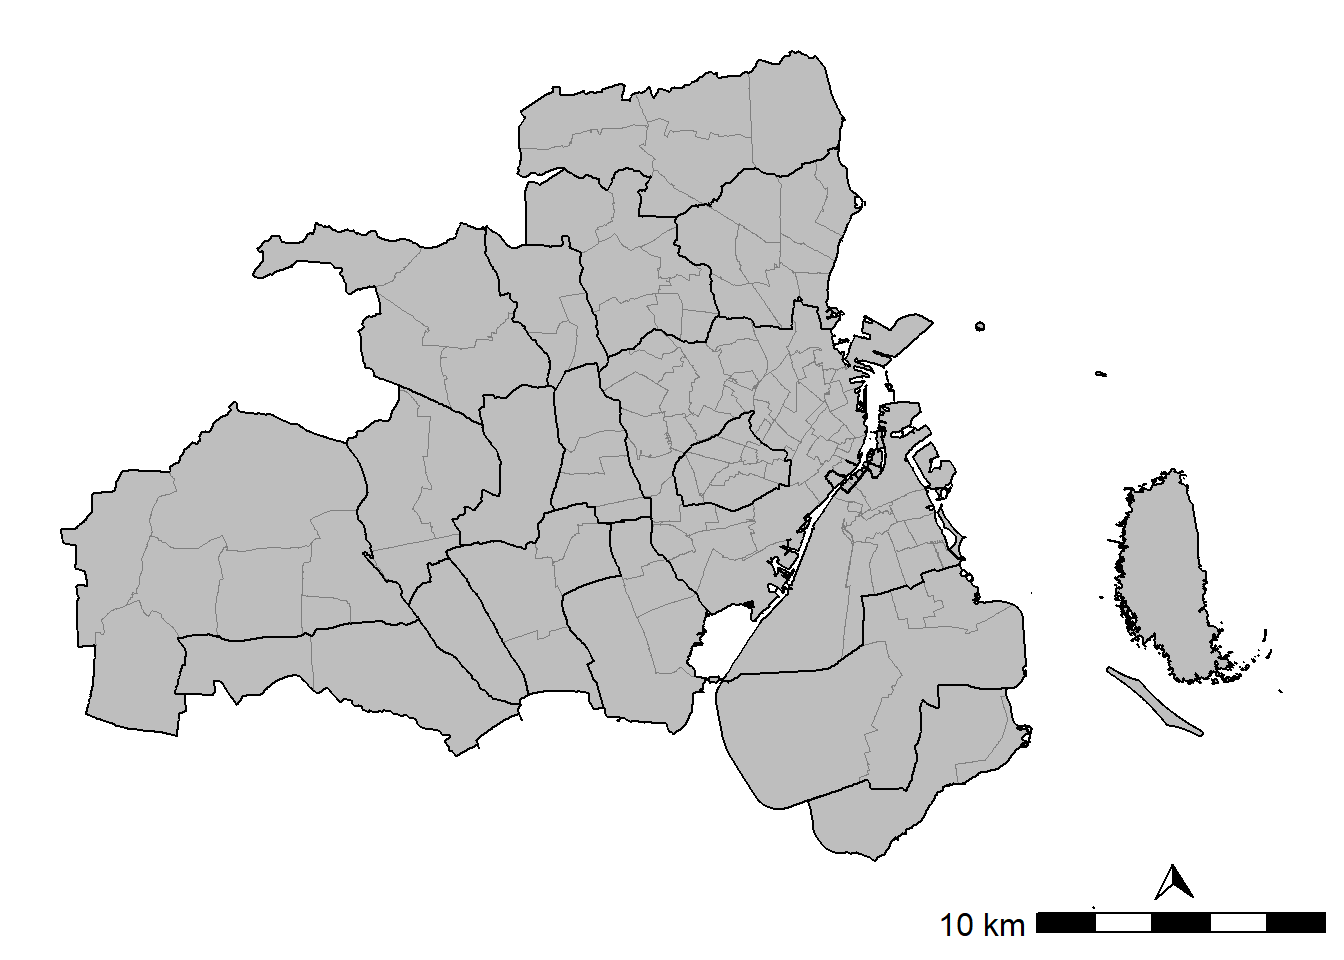
\includegraphics{CoDa_migr_cph_files/figure-latex/fig-cap-reg-prsh-1} 

}

\caption{Study area}\label{fig:fig-cap-reg-prsh}
\end{figure}

\hypertarget{population-data-at-parish-level}{%
\subsection{Population data at parish
level}\label{population-data-at-parish-level}}

Population data were uploaded from Denmark Statistics (i.e.~Table
\href{https://www.statbank.dk/statbank5a/SelectVarVal/Define.asp?MainTable=KMSTA001\&PLanguage=1\&PXSId=0\&wsid=cftree}{KMSTA001:
Population 1. January by parish, ancestry and National Church}).

\begin{Shaded}
\begin{Highlighting}[]
\DocumentationTok{\#\# Auxiliary functions for reading the data with the package *danstat*}

\CommentTok{\# Loop by year for getting DST data }
\NormalTok{  steps }\OtherTok{\textless{}{-}} \ControlFlowTok{function}\NormalTok{(year)\{}
\NormalTok{    var\_values }\OtherTok{\textless{}{-}} \FunctionTok{list}\NormalTok{(id\_region, id\_ancestry, year)}
\NormalTok{    var\_input }\OtherTok{\textless{}{-}}\NormalTok{ purrr}\SpecialCharTok{::}\FunctionTok{map2}\NormalTok{(}\AttributeTok{.x =}\NormalTok{ var\_codes,}
                             \AttributeTok{.y =}\NormalTok{ var\_values,}
                             \AttributeTok{.f =} \SpecialCharTok{\textasciitilde{}}\FunctionTok{list}\NormalTok{(}\AttributeTok{code =}\NormalTok{ .x, }\AttributeTok{values =}\NormalTok{ .y))}
    \FunctionTok{get\_data}\NormalTok{(id\_table, }\AttributeTok{variables =}\NormalTok{ var\_input)}
\NormalTok{  \}}
\end{Highlighting}
\end{Shaded}

\begin{Shaded}
\begin{Highlighting}[]
\DocumentationTok{\#\# Read and clean table KMSTA001}

\CommentTok{\# Table }
\NormalTok{id\_table }\OtherTok{\textless{}{-}} \StringTok{"KMSTA001"}
\NormalTok{var\_pop }\OtherTok{\textless{}{-}} \FunctionTok{get\_table\_metadata}\NormalTok{(}\AttributeTok{table\_id =}\NormalTok{ id\_table, }\AttributeTok{variables\_only =} \ConstantTok{TRUE}\NormalTok{)}

\CommentTok{\# Codes for var\_input}
\NormalTok{var\_codes }\OtherTok{\textless{}{-}} \FunctionTok{c}\NormalTok{(}\StringTok{"SOGN"}\NormalTok{, }\StringTok{"HERKOMST"}\NormalTok{, }\StringTok{"Tid"}\NormalTok{)}

\CommentTok{\# Values for var\_input}
\CommentTok{\# Region: parishes of the study area (i.e. cptl\_parish)}
\NormalTok{id\_region }\OtherTok{\textless{}{-}}\NormalTok{ cptl\_prsh}\SpecialCharTok{$}\NormalTok{prsh\_id }
\CommentTok{\# Ancestry}
\NormalTok{id\_ancestry }\OtherTok{\textless{}{-}} \ConstantTok{NA}
\CommentTok{\# Quarters}
\NormalTok{id\_year }\OtherTok{\textless{}{-}} \DecValTok{2020}  \CommentTok{\# vector with years}

\CommentTok{\# Read data (n parallel) }
\FunctionTok{plan}\NormalTok{(multisession, }\AttributeTok{workers =} \DecValTok{7}\NormalTok{)}
\NormalTok{cptl\_prsh\_ancestry\_read }\OtherTok{\textless{}{-}}\NormalTok{ id\_year }\SpecialCharTok{\%\textgreater{}\%}
  \FunctionTok{future\_map\_dfr}\NormalTok{(steps)  }
\FunctionTok{plan}\NormalTok{(}\StringTok{"default"}\NormalTok{)}

\CommentTok{\# Clean data }
\NormalTok{cptl\_prsh\_ancestry }\OtherTok{\textless{}{-}}\NormalTok{ cptl\_prsh\_ancestry\_read }\SpecialCharTok{\%\textgreater{}\%} 
  \CommentTok{\# Translate column names into English}
  \FunctionTok{rename}\NormalTok{(}\AttributeTok{parish =}\NormalTok{ SOGN,}
         \AttributeTok{ancestry =}\NormalTok{ HERKOMST,}
         \AttributeTok{year =}\NormalTok{ TID, }
         \AttributeTok{value =}\NormalTok{ INDHOLD) }\SpecialCharTok{\%\textgreater{}\%}
  \CommentTok{\# Get parish codes, names, and municipality names}
  \FunctionTok{separate}\NormalTok{(parish,}
           \FunctionTok{c}\NormalTok{(}\StringTok{"prsh\_id"}\NormalTok{, }\StringTok{"prsh\_name"}\NormalTok{, }\StringTok{"muni\_name"}\NormalTok{),}
           \AttributeTok{sep =} \StringTok{" "}\NormalTok{,}
           \AttributeTok{extra =} \StringTok{"drop"}\NormalTok{) }\SpecialCharTok{\%\textgreater{}\%} 
  \FunctionTok{mutate}\NormalTok{(}\AttributeTok{muni\_name =} \FunctionTok{gsub}\NormalTok{(}\StringTok{"}\SpecialCharTok{\textbackslash{}\textbackslash{}}\StringTok{("}\NormalTok{, }\StringTok{""}\NormalTok{, muni\_name)) }\SpecialCharTok{\%\textgreater{}\%} 
  \CommentTok{\# Make shorter names in ancestry}
  \FunctionTok{mutate}\NormalTok{(}\AttributeTok{ancestry =} \FunctionTok{case\_when}\NormalTok{(}
\NormalTok{    ancestry }\SpecialCharTok{==} \StringTok{"Persons of Danish origin"} \SpecialCharTok{\textasciitilde{}} \StringTok{"pop\_dan"}\NormalTok{,}
\NormalTok{    ancestry }\SpecialCharTok{==} \StringTok{"Immigrants from western countries"} \SpecialCharTok{\textasciitilde{}} \StringTok{"pop\_mi\_wst"}\NormalTok{,}
\NormalTok{    ancestry }\SpecialCharTok{==} \StringTok{"Immigrants from non{-}western countries"} \SpecialCharTok{\textasciitilde{}} \StringTok{"pop\_mi\_nwst"}\NormalTok{,}
\NormalTok{    ancestry }\SpecialCharTok{==} \StringTok{"Descendants from western countries"} \SpecialCharTok{\textasciitilde{}} \StringTok{"pop\_de\_wst"}\NormalTok{,}
\NormalTok{    ancestry }\SpecialCharTok{==} \StringTok{"Descendants from non{-}western countries"} \SpecialCharTok{\textasciitilde{}} \StringTok{"pop\_de\_nwst"}\NormalTok{), }
    \AttributeTok{ancestry =} \FunctionTok{factor}\NormalTok{(ancestry)) }\SpecialCharTok{\%\textgreater{}\%} 
  \CommentTok{\# Pivot (one row for peach parish and year)}
  \FunctionTok{pivot\_wider}\NormalTok{(}\AttributeTok{names\_from =}\NormalTok{ ancestry, }\AttributeTok{values\_from =}\NormalTok{ value) }\SpecialCharTok{\%\textgreater{}\%} 
  \CommentTok{\# Merge immigrants and their descendants (i.e. foreigners) }
  \FunctionTok{mutate}\NormalTok{(}\AttributeTok{pop\_frgn\_wst =}\NormalTok{ pop\_mi\_wst }\SpecialCharTok{+}\NormalTok{ pop\_de\_wst, }
         \AttributeTok{pop\_frgn\_nwst =}\NormalTok{ pop\_mi\_nwst }\SpecialCharTok{+}\NormalTok{ pop\_de\_nwst) }\SpecialCharTok{\%\textgreater{}\%} 
  \FunctionTok{select}\NormalTok{(}\SpecialCharTok{{-}}\FunctionTok{c}\NormalTok{(pop\_mi\_wst, pop\_de\_wst, pop\_mi\_nwst, pop\_de\_nwst)) }\SpecialCharTok{\%\textgreater{}\%} 
  \CommentTok{\# Add column with total population}
  \FunctionTok{mutate}\NormalTok{(}\AttributeTok{pop\_total =} \FunctionTok{select}\NormalTok{(., }\FunctionTok{starts\_with}\NormalTok{(}\StringTok{"pop\_"}\NormalTok{)) }\SpecialCharTok{\%\textgreater{}\%} \FunctionTok{rowSums}\NormalTok{()) }\SpecialCharTok{\%\textgreater{}\%} 
  \CommentTok{\# Put NA when pop\_* is 0}
  \FunctionTok{mutate}\NormalTok{(}\FunctionTok{across}\NormalTok{(}\FunctionTok{starts\_with}\NormalTok{(}\StringTok{"pop"}\NormalTok{), }\SpecialCharTok{\textasciitilde{}}\FunctionTok{ifelse}\NormalTok{(.x }\SpecialCharTok{==} \DecValTok{0}\NormalTok{, }\ConstantTok{NA}\NormalTok{, .x)))}

\CommentTok{\# Add the spatial information:}
\NormalTok{cptl\_prsh\_ancestry\_sf }\OtherTok{\textless{}{-}}\NormalTok{ cptl\_prsh }\SpecialCharTok{\%\textgreater{}\%}
  \FunctionTok{select}\NormalTok{(prsh\_id, prsh\_area\_km2) }\SpecialCharTok{\%\textgreater{}\%} 
  \FunctionTok{left\_join}\NormalTok{(cptl\_prsh\_ancestry, }\AttributeTok{by =} \FunctionTok{c}\NormalTok{(}\StringTok{"prsh\_id"}\NormalTok{)) }\SpecialCharTok{\%\textgreater{}\%} 
  \CommentTok{\# Population density}
  \FunctionTok{mutate}\NormalTok{(}\FunctionTok{across}\NormalTok{(}\FunctionTok{starts\_with}\NormalTok{(}\StringTok{"pop"}\NormalTok{), }\SpecialCharTok{\textasciitilde{}}\NormalTok{.x}\SpecialCharTok{/}\NormalTok{prsh\_area\_km2, }\AttributeTok{.names =} \StringTok{"\{.col\}\_km2"}\NormalTok{)) }\SpecialCharTok{\%\textgreater{}\%} 
  \CommentTok{\# Population in percentage   }
  \FunctionTok{mutate}\NormalTok{(}\FunctionTok{across}\NormalTok{(}\AttributeTok{.cols =} \FunctionTok{c}\NormalTok{(pop\_dan, pop\_frgn\_wst, pop\_frgn\_nwst, pop\_total),}
                \AttributeTok{.fns =} \SpecialCharTok{\textasciitilde{}} \DecValTok{100} \SpecialCharTok{*}\NormalTok{ .x }\SpecialCharTok{/}\NormalTok{ pop\_total,}
                \AttributeTok{.names =} \StringTok{"\{.col\}\_pct"}\NormalTok{)) }
\end{Highlighting}
\end{Shaded}

\hypertarget{housing-price}{%
\subsection{Housing price}\label{housing-price}}

We have got the housing prices from the Building and Dwelling Register
(\href{https://teknik.bbr.dk/forside}{BBR}). The individual data are not
free and we have therefore only saved here the summary statistics
(i.e.~mean and media values).

\begin{Shaded}
\begin{Highlighting}[]
\NormalTok{sum\_runits\_oft\_prices }\OtherTok{\textless{}{-}} \FunctionTok{readRDS}\NormalTok{(}\StringTok{"sum\_runits\_oft\_prices.rds"}\NormalTok{) }\SpecialCharTok{\%\textgreater{}\%} 
  \CommentTok{\# Remove NAs}
  \FunctionTok{drop\_na}\NormalTok{() }\SpecialCharTok{\%\textgreater{}\%} 
  \CommentTok{\# sf objects}
  \FunctionTok{st\_sf}\NormalTok{()}
\end{Highlighting}
\end{Shaded}

\hypertarget{analysis}{%
\section{Analysis}\label{analysis}}

\hypertarget{population-at-parish-level}{%
\subsection{Population at parish
level}\label{population-at-parish-level}}

Distribution of Danes, Western, and non-Western population (in
percentage over the total population in the parish).

\begin{Shaded}
\begin{Highlighting}[]
\NormalTok{cptl\_prsh\_ancestry\_sf }\SpecialCharTok{\%\textgreater{}\%}
  \FunctionTok{as\_tibble}\NormalTok{() }\SpecialCharTok{\%\textgreater{}\%} 
  \FunctionTok{select}\NormalTok{(pop\_dan\_pct, pop\_frgn\_nwst\_pct, pop\_frgn\_wst\_pct, }\SpecialCharTok{{-}}\NormalTok{geometry) }\SpecialCharTok{\%\textgreater{}\%}
  \FunctionTok{rename}\NormalTok{(}\AttributeTok{Danes =}\NormalTok{ pop\_dan\_pct,}
         \AttributeTok{Non\_Western =}\NormalTok{ pop\_frgn\_nwst\_pct,}
         \AttributeTok{Western =}\NormalTok{ pop\_frgn\_wst\_pct) }\SpecialCharTok{\%\textgreater{}\%} 
  \FunctionTok{pivot\_longer}\NormalTok{(}\AttributeTok{cols =} \FunctionTok{everything}\NormalTok{(),}
               \AttributeTok{names\_to =} \StringTok{"names"}\NormalTok{,}
               \AttributeTok{values\_to =} \StringTok{"value"}\NormalTok{) }\SpecialCharTok{\%\textgreater{}\%} 
  \CommentTok{\# Summary values}
  \FunctionTok{tbl\_summary}\NormalTok{(}\AttributeTok{by =}\NormalTok{ names,}
              \AttributeTok{type =} \FunctionTok{all\_continuous}\NormalTok{() }\SpecialCharTok{\textasciitilde{}} \StringTok{"continuous2"}\NormalTok{,}
              \AttributeTok{statistic =} \FunctionTok{all\_continuous}\NormalTok{() }\SpecialCharTok{\textasciitilde{}} \FunctionTok{c}\NormalTok{(}\StringTok{"\{mean\}"}\NormalTok{,}
                                               \StringTok{"\{median\}"}\NormalTok{,}
                                               \StringTok{"\{p25\} {-} \{p75\}"}\NormalTok{,}
                                               \StringTok{"\{min\} {-} \{max\}"}\NormalTok{),}
              \AttributeTok{missing =} \StringTok{"no"}\NormalTok{,}
              \AttributeTok{digits =} \FunctionTok{all\_continuous}\NormalTok{() }\SpecialCharTok{\textasciitilde{}} \DecValTok{1}\NormalTok{) }\SpecialCharTok{\%\textgreater{}\%}
  \FunctionTok{bold\_labels}\NormalTok{()}
\end{Highlighting}
\end{Shaded}

\begin{tabular}{l|l|l|l}
\hline
**Characteristic** & **Danes**, N = 127 & **Non\_Western**, N = 127 & **Western**, N = 127\\
\hline
\_\_value\_\_ &  &  & \\
\hline
Mean & 77.8 & 14.5 & 7.7\\
\hline
Median & 79.6 & 11.5 & 7.1\\
\hline
IQR & 72.9 - 84.3 & 7.7 - 17.7 & 4.9 - 9.7\\
\hline
Range & 21.2 - 94.6 & 2.7 - 69.9 & 2.7 - 19.9\\
\hline
\end{tabular}

\begin{Shaded}
\begin{Highlighting}[]
\NormalTok{cptl\_prsh\_ancestry\_sf }\SpecialCharTok{\%\textgreater{}\%}
  \FunctionTok{select}\NormalTok{(pop\_dan\_pct, pop\_frgn\_nwst\_pct, pop\_frgn\_wst\_pct) }\SpecialCharTok{\%\textgreater{}\%}
  \FunctionTok{rename}\NormalTok{(}\AttributeTok{Danes =}\NormalTok{ pop\_dan\_pct,}
         \AttributeTok{Non\_Western =}\NormalTok{ pop\_frgn\_nwst\_pct,}
         \AttributeTok{Western =}\NormalTok{ pop\_frgn\_wst\_pct) }\SpecialCharTok{\%\textgreater{}\%} 
  \FunctionTok{pivot\_longer}\NormalTok{(}\AttributeTok{cols =} \SpecialCharTok{{-}}\NormalTok{geometry,}
               \AttributeTok{names\_to =} \StringTok{"names"}\NormalTok{,}
               \AttributeTok{values\_to =} \StringTok{"value"}\NormalTok{) }\SpecialCharTok{\%\textgreater{}\%}
  \FunctionTok{st\_sf}\NormalTok{() }\SpecialCharTok{\%\textgreater{}\%} 
  \FunctionTok{ggplot}\NormalTok{() }\SpecialCharTok{+}
  \FunctionTok{geom\_sf}\NormalTok{(}\AttributeTok{data =}\NormalTok{ dk\_country\_crop, }\AttributeTok{fill =} \StringTok{"grey"}\NormalTok{) }\SpecialCharTok{+}  
  \FunctionTok{geom\_sf}\NormalTok{(}\FunctionTok{aes}\NormalTok{(}\AttributeTok{fill =}\NormalTok{ value ), }\AttributeTok{color =} \StringTok{"grey"}\NormalTok{, }\AttributeTok{size =} \FloatTok{0.05}\NormalTok{) }\SpecialCharTok{+}
  \FunctionTok{geom\_sf}\NormalTok{(}\AttributeTok{data =}\NormalTok{ cptl\_muni, }\AttributeTok{fill =} \ConstantTok{NA}\NormalTok{, }\AttributeTok{color =} \StringTok{"white"}\NormalTok{, }\AttributeTok{size =} \FloatTok{0.5}\NormalTok{) }\SpecialCharTok{+}
  \FunctionTok{scale\_fill\_viridis}\NormalTok{(}\AttributeTok{name =} \StringTok{"Percentage"}\NormalTok{,}
                     \AttributeTok{option =} \StringTok{"magma"}\NormalTok{,}
                     \AttributeTok{direction =} \SpecialCharTok{{-}}\DecValTok{1}\NormalTok{, }
                     \AttributeTok{limits =} \FunctionTok{c}\NormalTok{(}\DecValTok{0}\NormalTok{, }\DecValTok{100}\NormalTok{)) }\SpecialCharTok{+}
  \FunctionTok{theme\_void}\NormalTok{() }\SpecialCharTok{+}
  \FunctionTok{facet\_wrap}\NormalTok{(}\SpecialCharTok{\textasciitilde{}}\NormalTok{names, }\AttributeTok{ncol =} \DecValTok{1}\NormalTok{)}
\end{Highlighting}
\end{Shaded}

\begin{figure}[H]

{\centering 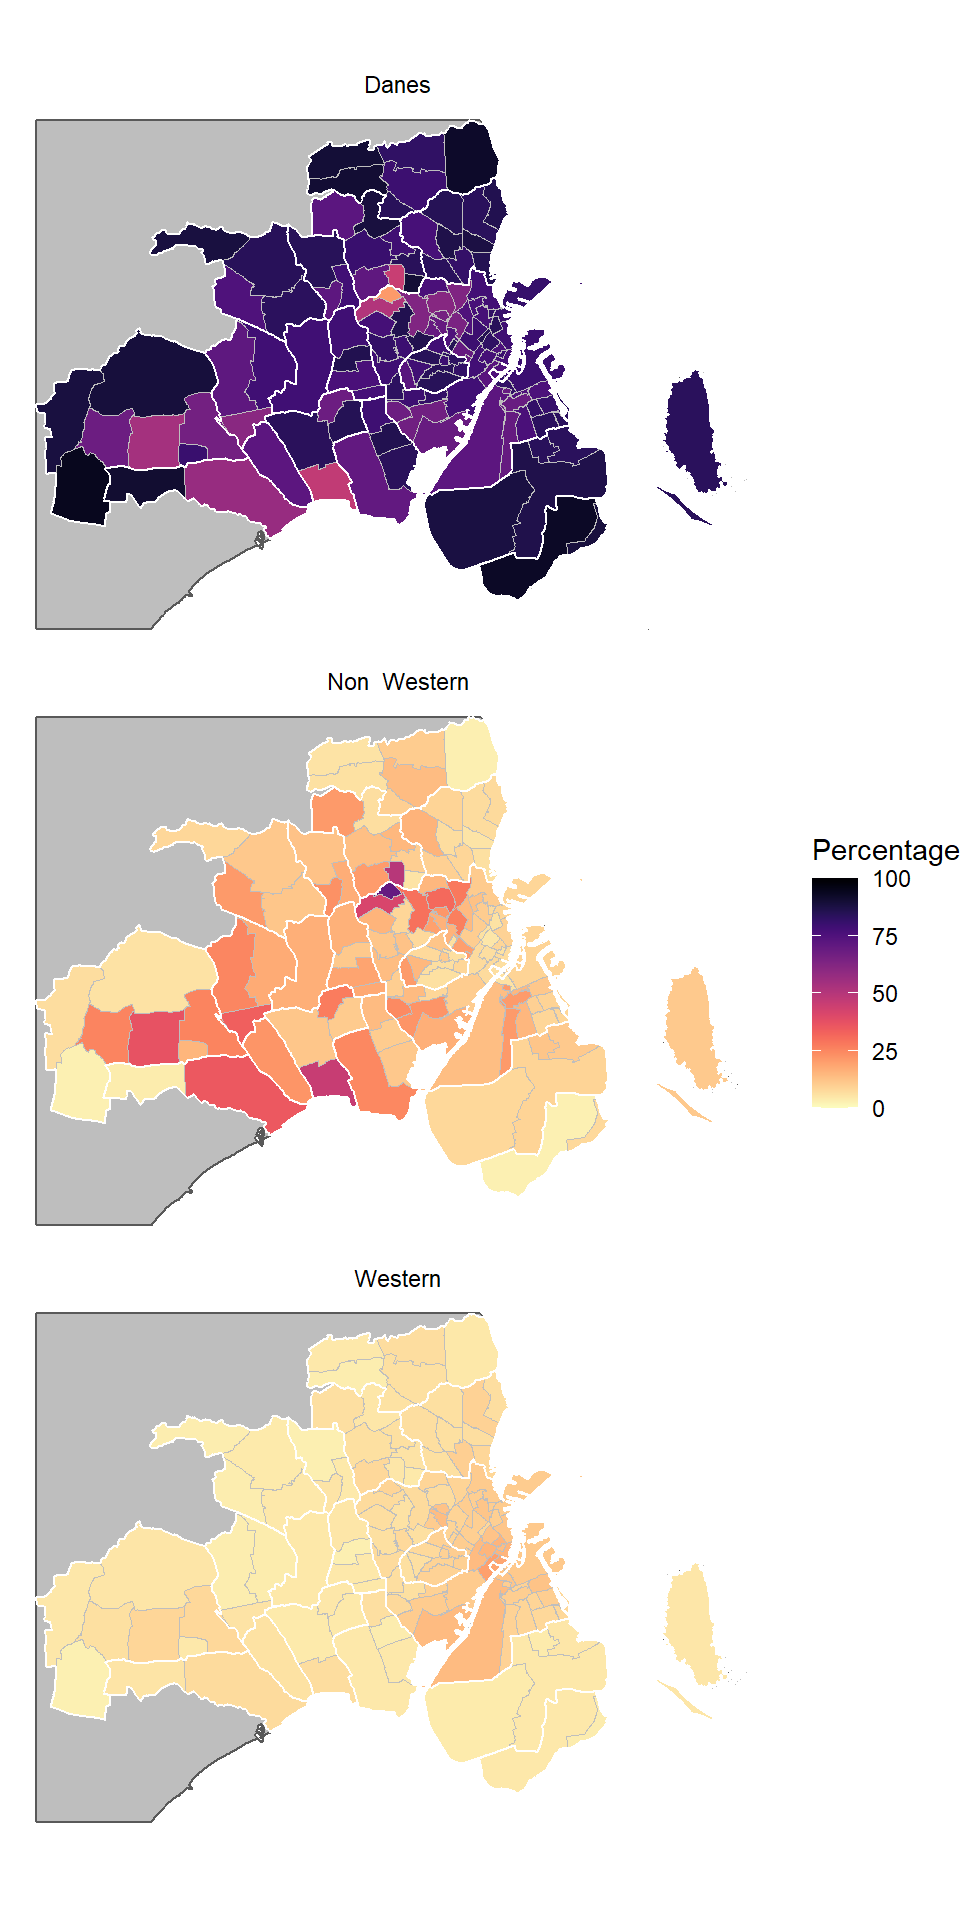
\includegraphics{CoDa_migr_cph_files/figure-latex/fig-pop-parish-1} 

}

\caption{Population distribution}\label{fig:fig-pop-parish}
\end{figure}

\hypertarget{housing-price-1}{%
\subsection{Housing price}\label{housing-price-1}}

Spatial distribution of median values.

\begin{Shaded}
\begin{Highlighting}[]
\FunctionTok{ggplot}\NormalTok{() }\SpecialCharTok{+}
  \FunctionTok{geom\_sf}\NormalTok{(}\AttributeTok{data =}\NormalTok{ dk\_country\_crop, }\AttributeTok{fill =} \StringTok{"grey"}\NormalTok{) }\SpecialCharTok{+} 
  \FunctionTok{geom\_sf}\NormalTok{(}\AttributeTok{data =}\NormalTok{ sum\_runits\_oft\_prices,}
          \FunctionTok{aes}\NormalTok{(}\AttributeTok{fill =} \FunctionTok{cut\_number}\NormalTok{(median\_kDKK\_m2,}
                                \AttributeTok{n =} \DecValTok{10}\NormalTok{,}
                                \AttributeTok{ordered\_result =} \ConstantTok{TRUE}\NormalTok{,}
                                \AttributeTok{dig.lab =} \DecValTok{0}\NormalTok{)),}
          \AttributeTok{color =} \StringTok{"grey"}\NormalTok{,}
          \AttributeTok{size =} \FloatTok{0.05}\NormalTok{) }\SpecialCharTok{+}
  \FunctionTok{geom\_sf}\NormalTok{(}\AttributeTok{data =}\NormalTok{ cptl\_muni, }\AttributeTok{fill =} \ConstantTok{NA}\NormalTok{, }\AttributeTok{color =} \StringTok{"white"}\NormalTok{, }\AttributeTok{size =} \FloatTok{0.5}\NormalTok{) }\SpecialCharTok{+}
  \FunctionTok{scale\_fill\_viridis\_d}\NormalTok{(}\AttributeTok{name =} \StringTok{"Percentiles}\SpecialCharTok{\textbackslash{}n}\StringTok{[kDKK/m2]"}\NormalTok{,}
                     \AttributeTok{option =} \StringTok{"magma"}\NormalTok{,}
                     \AttributeTok{direction =} \SpecialCharTok{{-}}\DecValTok{1}\NormalTok{) }\SpecialCharTok{+}
  \FunctionTok{labs}\NormalTok{(}\AttributeTok{x =} \StringTok{""}\NormalTok{,}
       \AttributeTok{y =} \StringTok{""}\NormalTok{) }\SpecialCharTok{+}
  \FunctionTok{theme\_void}\NormalTok{() }\SpecialCharTok{+}
  \FunctionTok{guides}\NormalTok{(}\AttributeTok{fill =} \FunctionTok{guide\_legend}\NormalTok{(}\AttributeTok{reverse =} \ConstantTok{TRUE}\NormalTok{))}
\end{Highlighting}
\end{Shaded}

\begin{figure}[H]

{\centering 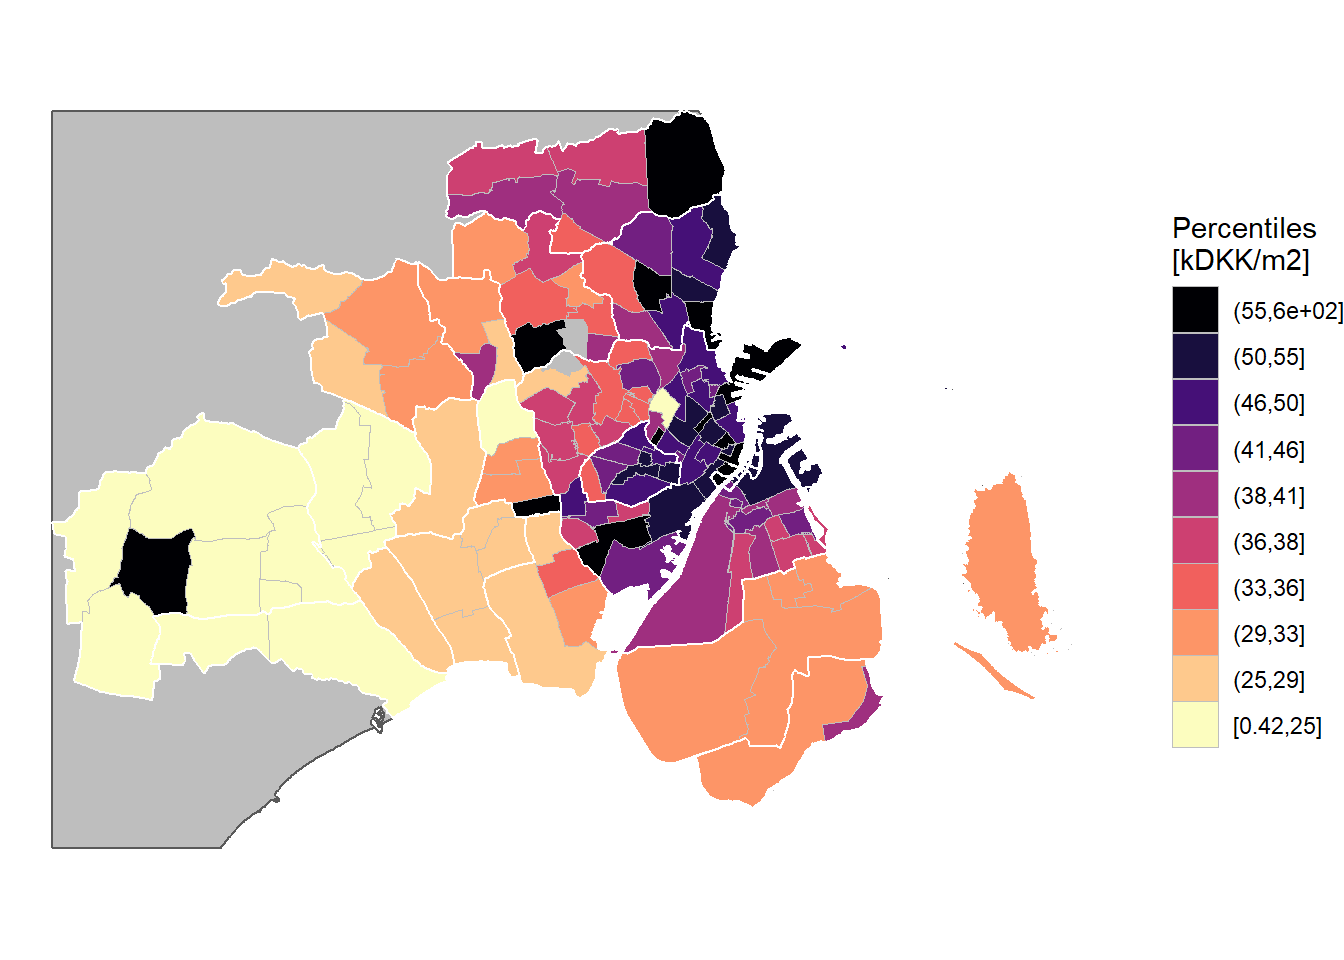
\includegraphics{CoDa_migr_cph_files/figure-latex/fig-prices-runits-parish-b-1} 

}

\caption{Median house prices in the ordinary free trade}\label{fig:fig-prices-runits-parish-b}
\end{figure}

The summary descriptive statistics of the housing prices by parishes:

\begin{Shaded}
\begin{Highlighting}[]
\CommentTok{\# Create variable labels of the variables to be printed in the table}
\NormalTok{labelled}\SpecialCharTok{::}\FunctionTok{var\_label}\NormalTok{(sum\_runits\_oft\_prices}\SpecialCharTok{$}\NormalTok{n\_runits\_oft)   }\OtherTok{\textless{}{-}} \StringTok{"N. houses in the ordinary free trade"}
\NormalTok{labelled}\SpecialCharTok{::}\FunctionTok{var\_label}\NormalTok{(sum\_runits\_oft\_prices}\SpecialCharTok{$}\NormalTok{mean\_kDKK\_m2)   }\OtherTok{\textless{}{-}} \StringTok{"Mean (kDKK/m2)"}
\NormalTok{labelled}\SpecialCharTok{::}\FunctionTok{var\_label}\NormalTok{(sum\_runits\_oft\_prices}\SpecialCharTok{$}\NormalTok{median\_kDKK\_m2) }\OtherTok{\textless{}{-}} \StringTok{"Median (kDKK/m2)"}

\CommentTok{\# Summary table}
\NormalTok{sum\_runits\_oft\_prices }\SpecialCharTok{\%\textgreater{}\%} 
  \FunctionTok{as\_tibble}\NormalTok{() }\SpecialCharTok{\%\textgreater{}\%} 
  \CommentTok{\# Select variables of interest}
  \FunctionTok{select}\NormalTok{(n\_runits\_oft, mean\_kDKK\_m2,  median\_kDKK\_m2) }\SpecialCharTok{\%\textgreater{}\%}
  \CommentTok{\# Summary values}
  \FunctionTok{tbl\_summary}\NormalTok{(}\AttributeTok{type =} \FunctionTok{all\_continuous}\NormalTok{() }\SpecialCharTok{\textasciitilde{}} \StringTok{"continuous2"}\NormalTok{,}
              \AttributeTok{statistic =} \FunctionTok{all\_continuous}\NormalTok{() }\SpecialCharTok{\textasciitilde{}} \FunctionTok{c}\NormalTok{(}\StringTok{"\{mean\}"}\NormalTok{,}
                                               \StringTok{"\{median\}"}\NormalTok{,}
                                               \StringTok{"\{p25\} {-} \{p75\}"}\NormalTok{,}
                                               \StringTok{"\{min\} {-} \{max\}"}\NormalTok{),}
              \AttributeTok{missing =} \StringTok{"no"}\NormalTok{,}
              \AttributeTok{digits =} \FunctionTok{all\_continuous}\NormalTok{() }\SpecialCharTok{\textasciitilde{}} \DecValTok{1}\NormalTok{) }\SpecialCharTok{\%\textgreater{}\%}
  \FunctionTok{bold\_labels}\NormalTok{()}
\end{Highlighting}
\end{Shaded}

\begin{tabular}{l|l}
\hline
**Characteristic** & **N = 125**\\
\hline
\_\_N. houses in the ordinary free trade\_\_ & \\
\hline
Mean & 150.1\\
\hline
Median & 127.0\\
\hline
IQR & 85.0 - 182.0\\
\hline
Range & 7.0 - 637.0\\
\hline
\_\_Mean (kDKK/m2)\_\_ & \\
\hline
Mean & 82.8\\
\hline
Median & 42.3\\
\hline
IQR & 33.2 - 61.2\\
\hline
Range & 22.1 - 1,132.9\\
\hline
\_\_Median (kDKK/m2)\_\_ & \\
\hline
Mean & 46.2\\
\hline
Median & 38.0\\
\hline
IQR & 31.1 - 47.4\\
\hline
Range & 0.4 - 602.6\\
\hline
\end{tabular}

\hypertarget{compositional-data-analysis}{%
\subsection{Compositional data
analysis}\label{compositional-data-analysis}}

Ternary representation of population distribution.

\begin{Shaded}
\begin{Highlighting}[]
\CommentTok{\# Make colours}
\NormalTok{tric }\OtherTok{\textless{}{-}}\NormalTok{ tricolore}\SpecialCharTok{::}\FunctionTok{Tricolore}\NormalTok{(cptl\_prsh\_ancestry\_sf,}
                             \AttributeTok{p1 =} \StringTok{"pop\_dan"}\NormalTok{,}
                             \AttributeTok{p2 =} \StringTok{"pop\_frgn\_wst"}\NormalTok{,}
                             \AttributeTok{p3 =} \StringTok{"pop\_frgn\_nwst"}\NormalTok{,}
                             \AttributeTok{breaks =} \ConstantTok{Inf}\NormalTok{,}
                             \AttributeTok{show\_data =} \ConstantTok{FALSE}\NormalTok{,}
                             \AttributeTok{center =} \ConstantTok{NA}\NormalTok{,}
                             \AttributeTok{hue =} \DecValTok{2}\SpecialCharTok{/}\DecValTok{12}\NormalTok{,}
                             \AttributeTok{lightness =} \DecValTok{1}\NormalTok{,}
                             \AttributeTok{chroma =} \DecValTok{1}\NormalTok{)}

\CommentTok{\# Add columns with colours}
\NormalTok{cptl\_prsh\_ancestry\_sf }\OtherTok{\textless{}{-}} \FunctionTok{mutate}\NormalTok{(cptl\_prsh\_ancestry\_sf, }\AttributeTok{pop\_rgb =}\NormalTok{ tric}\SpecialCharTok{$}\NormalTok{rgb)}

\CommentTok{\# Legend}
\NormalTok{p\_legend }\OtherTok{\textless{}{-}}\NormalTok{ tric}\SpecialCharTok{$}\NormalTok{key }\SpecialCharTok{+}
  \FunctionTok{geom\_point}\NormalTok{(}\AttributeTok{data =}\NormalTok{ cptl\_prsh\_ancestry\_sf,}
             \FunctionTok{aes}\NormalTok{(}\AttributeTok{x =}\NormalTok{ pop\_dan, }\AttributeTok{y =}\NormalTok{ pop\_frgn\_wst, }\AttributeTok{z =}\NormalTok{ pop\_frgn\_nwst),}
             \AttributeTok{shape =} \DecValTok{16}\NormalTok{,}
             \AttributeTok{size =} \FloatTok{0.2}\NormalTok{) }\SpecialCharTok{+}
  \FunctionTok{labs}\NormalTok{(}\AttributeTok{L =} \StringTok{"\% Danes"}\NormalTok{,}
       \AttributeTok{T =} \StringTok{"\% Wst"}\NormalTok{,}
       \AttributeTok{R =} \StringTok{"\% Non{-}wst"}\NormalTok{) }\SpecialCharTok{+}
  \FunctionTok{theme}\NormalTok{(}\AttributeTok{axis.title =} \FunctionTok{element\_text}\NormalTok{(}\AttributeTok{size =} \DecValTok{5}\NormalTok{, }\AttributeTok{face =} \StringTok{"bold"}\NormalTok{),}
        \AttributeTok{axis.text  =} \FunctionTok{element\_text}\NormalTok{(}\AttributeTok{size =} \DecValTok{5}\NormalTok{))}

\CommentTok{\# Label Husumvold, Haralds and Tingbjerg}
\NormalTok{prsh\_lbls }\OtherTok{\textless{}{-}}\NormalTok{ cptl\_prsh\_ancestry\_sf }\SpecialCharTok{\%\textgreater{}\%} 
  \FunctionTok{filter}\NormalTok{(prsh\_name }\SpecialCharTok{\%in\%} \FunctionTok{c}\NormalTok{(}\StringTok{"Husumvold"}\NormalTok{, }\StringTok{"Haralds"}\NormalTok{, }\StringTok{"Tingbjerg"}\NormalTok{))}

\CommentTok{\# Map}
\FunctionTok{ggplot}\NormalTok{() }\SpecialCharTok{+}
  \FunctionTok{geom\_sf}\NormalTok{(}\AttributeTok{data =}\NormalTok{ dk\_country\_crop,}
          \FunctionTok{aes}\NormalTok{(}\AttributeTok{geometry =}\NormalTok{ geometry),}
          \AttributeTok{fill =} \StringTok{"grey"}\NormalTok{) }\SpecialCharTok{+}
  \FunctionTok{geom\_sf}\NormalTok{(}\AttributeTok{data =}\NormalTok{ cptl\_prsh\_ancestry\_sf,}
          \FunctionTok{aes}\NormalTok{(}\AttributeTok{fill =}\NormalTok{ pop\_rgb, }\AttributeTok{geometry =}\NormalTok{ geometry),}
          \AttributeTok{size =} \FloatTok{0.05}\NormalTok{) }\SpecialCharTok{+}
  \FunctionTok{scale\_fill\_identity}\NormalTok{() }\SpecialCharTok{+}
  \FunctionTok{geom\_sf}\NormalTok{(}\AttributeTok{data =}\NormalTok{ cptl\_muni,}
          \FunctionTok{aes}\NormalTok{(}\AttributeTok{geometry =}\NormalTok{ geometry),}
          \AttributeTok{fill =} \ConstantTok{NA}\NormalTok{,}
          \AttributeTok{color =} \StringTok{"white"}\NormalTok{,}
          \AttributeTok{size =} \FloatTok{0.5}\NormalTok{) }\SpecialCharTok{+}
  \FunctionTok{geom\_sf\_label\_repel}\NormalTok{(}\AttributeTok{data =}\NormalTok{ prsh\_lbls,}
                      \FunctionTok{aes}\NormalTok{(}\AttributeTok{label =}\NormalTok{ prsh\_name),}
                      \AttributeTok{force =} \DecValTok{15}\NormalTok{,}
                      \AttributeTok{nudge\_y =}   \DecValTok{7000}\NormalTok{,}
                      \AttributeTok{nudge\_x =} \SpecialCharTok{{-}}\DecValTok{10000}\NormalTok{,}
                      \AttributeTok{seed =} \DecValTok{15}\NormalTok{) }\SpecialCharTok{+}
  \FunctionTok{theme\_void}\NormalTok{() }\SpecialCharTok{+}
  \FunctionTok{annotation\_custom}\NormalTok{(ggtern}\SpecialCharTok{::}\FunctionTok{ggplotGrob}\NormalTok{(p\_legend) ,}
                    \AttributeTok{xmin =}  \DecValTok{730000}\NormalTok{,}
                    \AttributeTok{xmax =}  \DecValTok{742000}\NormalTok{,}
                    \AttributeTok{ymin =} \DecValTok{6178000}\NormalTok{,}
                    \AttributeTok{ymax =} \DecValTok{6190000}\NormalTok{)}
\end{Highlighting}
\end{Shaded}

\begin{figure}[H]

{\centering 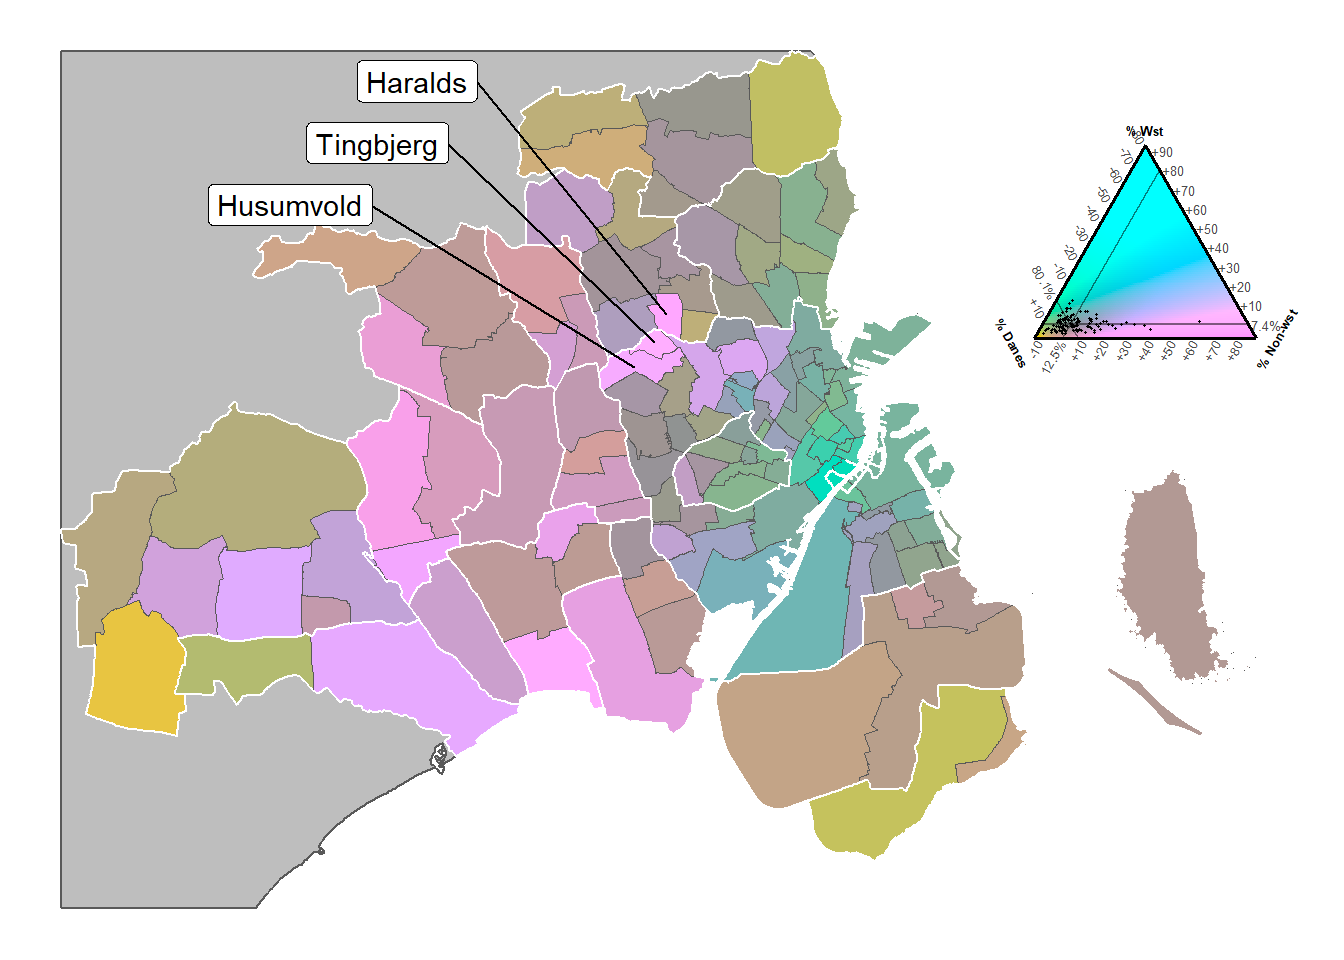
\includegraphics{CoDa_migr_cph_files/figure-latex/fig-tern-pop-1} 

}

\caption{Population distribution in 2020}\label{fig:fig-tern-pop}
\end{figure}

\hypertarget{balances}{%
\subsubsection{Balances}\label{balances}}

Transform data to CoDa format.

\begin{Shaded}
\begin{Highlighting}[]
\CommentTok{\# Transform to CoDa format}
\NormalTok{dat\_acomp }\OtherTok{\textless{}{-}}\NormalTok{ cptl\_prsh\_ancestry\_sf }\SpecialCharTok{\%\textgreater{}\%}
  \FunctionTok{select}\NormalTok{(prsh\_id, pop\_dan, pop\_frgn\_nwst, pop\_frgn\_wst) }\SpecialCharTok{\%\textgreater{}\%}
  \FunctionTok{rename}\NormalTok{(}\AttributeTok{dan =}\NormalTok{ pop\_dan, }
         \AttributeTok{nwst =}\NormalTok{ pop\_frgn\_nwst,}
         \AttributeTok{wst =}\NormalTok{ pop\_frgn\_wst) }\SpecialCharTok{\%\textgreater{}\%} 
  \FunctionTok{as\_tibble}\NormalTok{() }\SpecialCharTok{\%\textgreater{}\%}
  \FunctionTok{drop\_na}\NormalTok{() }\SpecialCharTok{\%\textgreater{}\%} 
  \FunctionTok{select}\NormalTok{(}\SpecialCharTok{{-}}\NormalTok{geometry) }\SpecialCharTok{\%\textgreater{}\%}
  \CommentTok{\# Close dataset}
  \FunctionTok{clo}\NormalTok{(}\AttributeTok{parts =} \FunctionTok{c}\NormalTok{(}\StringTok{"dan"}\NormalTok{, }\StringTok{"nwst"}\NormalTok{, }\StringTok{"wst"}\NormalTok{),}
      \AttributeTok{total =} \DecValTok{100}\NormalTok{) }\SpecialCharTok{\%\textgreater{}\%} 
  \CommentTok{\# CoDa}
  \FunctionTok{acomp}\NormalTok{()}
\end{Highlighting}
\end{Shaded}

PCA with clr transformations.

\begin{Shaded}
\begin{Highlighting}[]
\CommentTok{\# PCA}
\NormalTok{pc }\OtherTok{\textless{}{-}} \FunctionTok{princomp}\NormalTok{(dat\_acomp)}

\NormalTok{pca\_importance }\OtherTok{\textless{}{-}} \ControlFlowTok{function}\NormalTok{(x) \{}
\NormalTok{  vars }\OtherTok{\textless{}{-}}\NormalTok{ x}\SpecialCharTok{$}\NormalTok{sdev}\SpecialCharTok{\^{}}\DecValTok{2}
\NormalTok{  vars }\OtherTok{\textless{}{-}}\NormalTok{ vars}\SpecialCharTok{/}\FunctionTok{sum}\NormalTok{(vars)}
  \FunctionTok{rbind}\NormalTok{(}\StringTok{"Standard deviation"} \OtherTok{=}\NormalTok{ x}\SpecialCharTok{$}\NormalTok{sdev,}
        \StringTok{"Proportion of Variance"} \OtherTok{=}\NormalTok{ vars,}
        \StringTok{"Cumulative Proportion"} \OtherTok{=} \FunctionTok{cumsum}\NormalTok{(vars))}
\NormalTok{\}}

\FunctionTok{pca\_importance}\NormalTok{(}\FunctionTok{summary}\NormalTok{(pc)) }\SpecialCharTok{\%\textgreater{}\%} 
  \FunctionTok{kbl}\NormalTok{(}\AttributeTok{caption =} \StringTok{"Importance of components"}\NormalTok{,}
      \AttributeTok{digits =} \DecValTok{3}\NormalTok{) }\SpecialCharTok{\%\textgreater{}\%}
  \FunctionTok{kable\_styling}\NormalTok{()}
\end{Highlighting}
\end{Shaded}

\begin{table}

\caption{\label{tab:prsh-CoDa-PCA}Importance of components}
\centering
\begin{tabular}[t]{l|r|r}
\hline
  & Comp.1 & Comp.2\\
\hline
Standard deviation & 0.574 & 0.353\\
\hline
Proportion of Variance & 0.726 & 0.274\\
\hline
Cumulative Proportion & 0.726 & 1.000\\
\hline
\end{tabular}
\end{table}

Biplot and balance-dendrogram:

\begin{Shaded}
\begin{Highlighting}[]
\FunctionTok{par}\NormalTok{(}\AttributeTok{mfrow =} \FunctionTok{c}\NormalTok{(}\DecValTok{1}\NormalTok{, }\DecValTok{2}\NormalTok{))}
\FunctionTok{coloredBiplot}\NormalTok{(}\AttributeTok{x =}\NormalTok{ pc,}
              \AttributeTok{pc.biplot =}\NormalTok{ T,}
              \AttributeTok{xlabs.pc =} \FunctionTok{c}\NormalTok{(}\DecValTok{1}\NormalTok{, }\DecValTok{2}\NormalTok{, }\DecValTok{3}\NormalTok{),}
              \AttributeTok{xlabs.col =} \DecValTok{2}\SpecialCharTok{:}\DecValTok{4}\NormalTok{,}
              \AttributeTok{col =} \StringTok{"black"}\NormalTok{,}
              \AttributeTok{xlab =} \StringTok{"Comp. 1 (73\%)"}\NormalTok{,}
              \AttributeTok{ylab =} \StringTok{"Comp. 1 (27\%)"}\NormalTok{,}
              \AttributeTok{xlim =} \FunctionTok{c}\NormalTok{(}\SpecialCharTok{{-}}\FloatTok{3.5}\NormalTok{, }\DecValTok{2}\NormalTok{))}
\FunctionTok{title}\NormalTok{(}\AttributeTok{outer =}\NormalTok{ T,}
      \AttributeTok{adj =} \FloatTok{0.05}\NormalTok{,}
      \AttributeTok{main =} \StringTok{"A"}\NormalTok{,}
      \AttributeTok{cex =} \FloatTok{1.1}\NormalTok{,}
      \AttributeTok{col =} \StringTok{"black"}\NormalTok{,}
      \AttributeTok{font =} \DecValTok{2}\NormalTok{,}
      \AttributeTok{line =} \SpecialCharTok{{-}}\DecValTok{2}\NormalTok{)}

\CommentTok{\# Dendrogram balances}
\NormalTok{signary }\OtherTok{\textless{}{-}} \FunctionTok{t}\NormalTok{(}\FunctionTok{matrix}\NormalTok{( }\FunctionTok{c}\NormalTok{(}\DecValTok{1}\NormalTok{, }\SpecialCharTok{{-}}\DecValTok{1}\NormalTok{,  }\DecValTok{1}\NormalTok{,}
                       \DecValTok{1}\NormalTok{,  }\DecValTok{0}\NormalTok{, }\SpecialCharTok{{-}}\DecValTok{1}\NormalTok{),}
                     \AttributeTok{ncol =} \DecValTok{3}\NormalTok{,}
                     \AttributeTok{nrow =} \DecValTok{2}\NormalTok{,}
                     \AttributeTok{byrow =} \ConstantTok{TRUE}\NormalTok{))}
\FunctionTok{CoDaDendrogram}\NormalTok{(}\AttributeTok{X =}\NormalTok{ dat\_acomp,}
               \AttributeTok{signary =}\NormalTok{ signary,}
               \AttributeTok{col =} \StringTok{"black"}\NormalTok{,}
               \AttributeTok{main =} \StringTok{"CoDa Dendrogram"}\NormalTok{)}
\FunctionTok{title}\NormalTok{(}\AttributeTok{outer =}\NormalTok{ T,}
      \AttributeTok{adj =} \FloatTok{0.55}\NormalTok{,}
      \AttributeTok{main =} \StringTok{"B"}\NormalTok{,}
      \AttributeTok{cex =} \FloatTok{1.1}\NormalTok{,}
      \AttributeTok{col =} \StringTok{"black"}\NormalTok{,}
      \AttributeTok{font =} \DecValTok{2}\NormalTok{,}
      \AttributeTok{line =} \SpecialCharTok{{-}}\DecValTok{2}\NormalTok{)}
\end{Highlighting}
\end{Shaded}

\begin{figure}[H]

{\centering 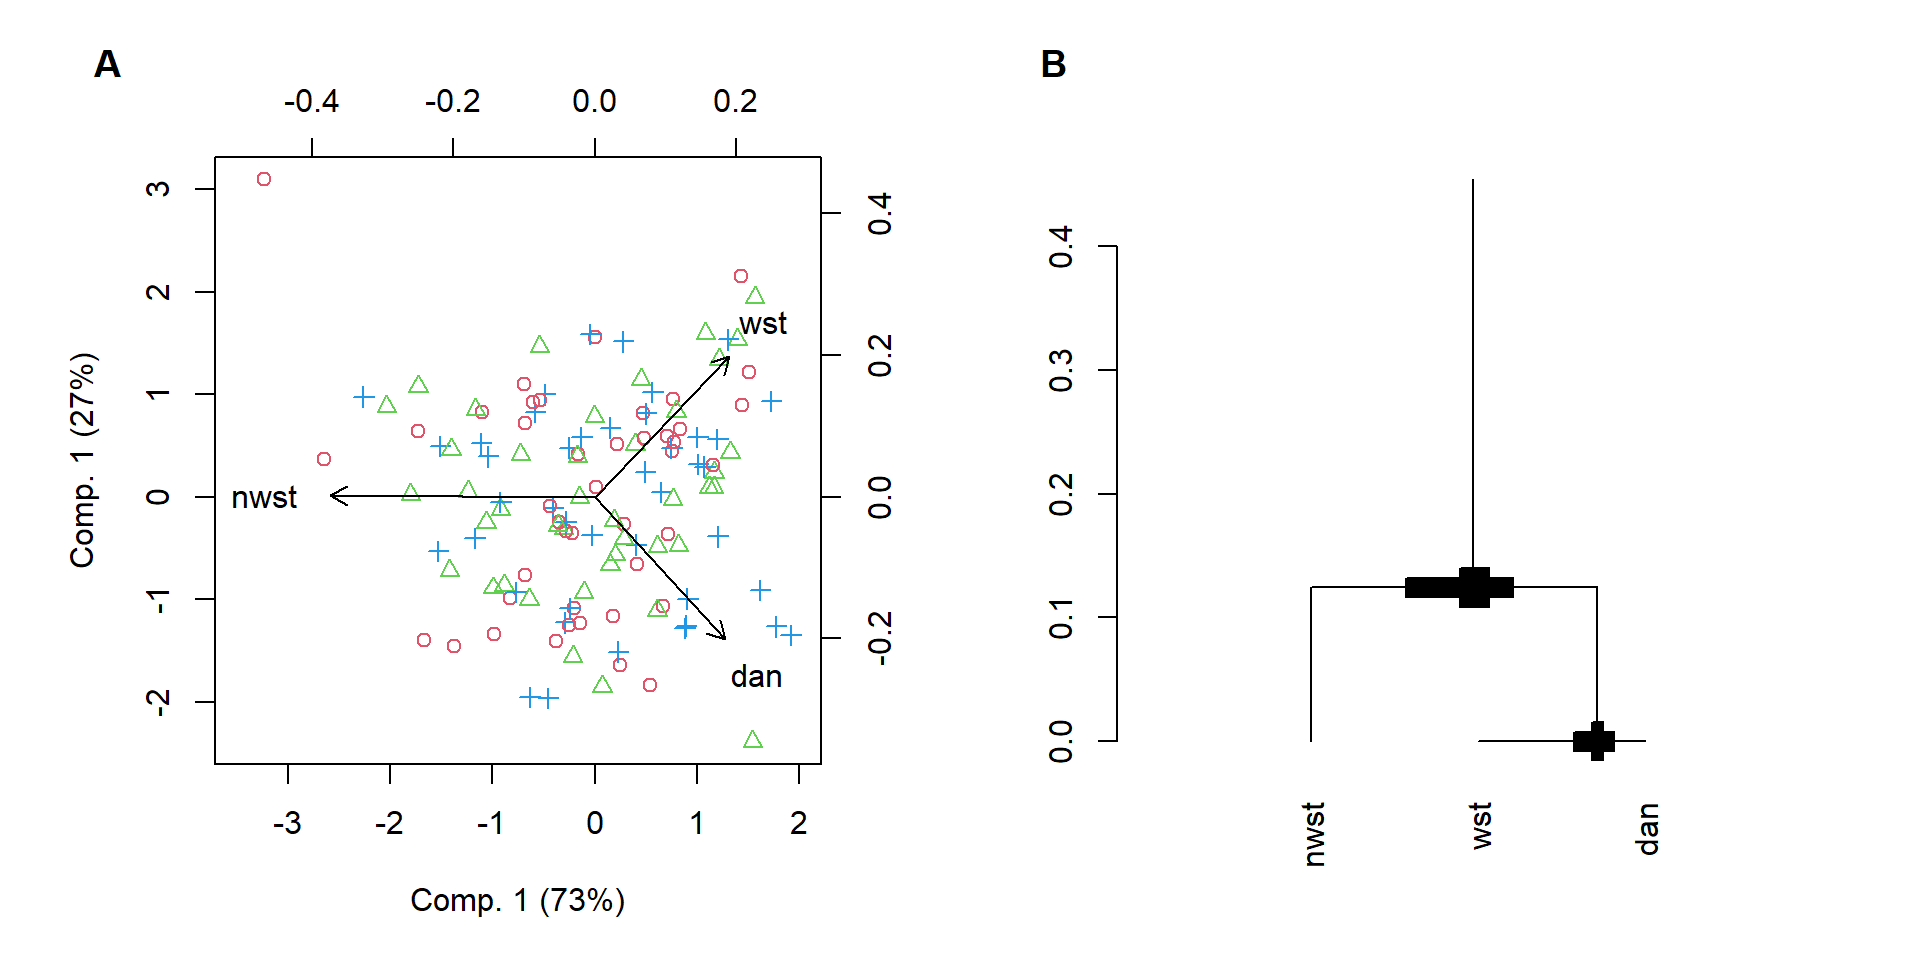
\includegraphics{CoDa_migr_cph_files/figure-latex/fig-prsh-CoDa-PCA-1} 

}

\caption{Biplot of clr transfomation and balance dendrogram}\label{fig:fig-prsh-CoDa-PCA}
\end{figure}

Add balances (b1 and b2) to the dataset:

\begin{Shaded}
\begin{Highlighting}[]
\NormalTok{cptl\_prsh\_ancestry\_sf }\OtherTok{\textless{}{-}}\NormalTok{ cptl\_prsh\_ancestry\_sf }\SpecialCharTok{\%\textgreater{}\%}
  \FunctionTok{mutate}\NormalTok{(}\AttributeTok{b1 =} \FunctionTok{sqrt}\NormalTok{(}\DecValTok{2}\SpecialCharTok{/}\DecValTok{3}\NormalTok{) }\SpecialCharTok{*} \FunctionTok{log}\NormalTok{( ((pop\_dan }\SpecialCharTok{*}\NormalTok{ pop\_frgn\_wst)}\SpecialCharTok{\^{}}\FloatTok{0.5}\NormalTok{) }\SpecialCharTok{/}\NormalTok{ (pop\_frgn\_nwst)),}
         \AttributeTok{b2 =} \FunctionTok{sqrt}\NormalTok{(}\DecValTok{1}\SpecialCharTok{/}\DecValTok{2}\NormalTok{) }\SpecialCharTok{*} \FunctionTok{log}\NormalTok{(pop\_dan }\SpecialCharTok{/}\NormalTok{ pop\_frgn\_wst))}
\end{Highlighting}
\end{Shaded}

Higher values of b1 indicate less non-Western population while higher
values of b2 indicate less western migrants:

\begin{Shaded}
\begin{Highlighting}[]
\NormalTok{cptl\_prsh\_ancestry\_sf }\SpecialCharTok{\%\textgreater{}\%} 
  \FunctionTok{as\_tibble}\NormalTok{() }\SpecialCharTok{\%\textgreater{}\%} 
  \FunctionTok{select}\NormalTok{(pop\_dan\_pct, pop\_frgn\_wst\_pct, pop\_frgn\_nwst\_pct, b1, b2, }\SpecialCharTok{{-}}\NormalTok{geometry) }\SpecialCharTok{\%\textgreater{}\%} 
  \FunctionTok{pivot\_longer}\NormalTok{(}\AttributeTok{cols =} \SpecialCharTok{{-}}\FunctionTok{c}\NormalTok{(b1, b2),}
               \AttributeTok{names\_to =} \StringTok{"pop"}\NormalTok{,}
               \AttributeTok{values\_to =} \StringTok{"percentage"}\NormalTok{) }\SpecialCharTok{\%\textgreater{}\%}
  \FunctionTok{pivot\_longer}\NormalTok{(}\AttributeTok{cols =} \SpecialCharTok{{-}}\FunctionTok{c}\NormalTok{(pop, percentage),}
               \AttributeTok{names\_to =} \StringTok{"balance"}\NormalTok{,}
               \AttributeTok{values\_to =} \StringTok{"value"}\NormalTok{) }\SpecialCharTok{\%\textgreater{}\%} 
  \FunctionTok{mutate}\NormalTok{(}\AttributeTok{pop =} \FunctionTok{factor}\NormalTok{(pop,}
                      \AttributeTok{levels =} \FunctionTok{c}\NormalTok{(}\StringTok{"pop\_dan\_pct"}\NormalTok{,}
                                 \StringTok{"pop\_frgn\_wst\_pct"}\NormalTok{,}
                                 \StringTok{"pop\_frgn\_nwst\_pct"}\NormalTok{),}
                      \AttributeTok{labels =} \FunctionTok{c}\NormalTok{(}\StringTok{"Danes"}\NormalTok{,}
                                 \StringTok{"Western"}\NormalTok{,}
                                 \StringTok{"non{-}Western"}\NormalTok{))) }\SpecialCharTok{\%\textgreater{}\%}
  \FunctionTok{ggplot}\NormalTok{() }\SpecialCharTok{+}
  \FunctionTok{geom\_point}\NormalTok{(}\FunctionTok{aes}\NormalTok{(}\AttributeTok{x =}\NormalTok{ value,}
                 \AttributeTok{y =}\NormalTok{ percentage)) }\SpecialCharTok{+}
  \FunctionTok{labs}\NormalTok{(}\AttributeTok{y =} \StringTok{"Percentage [\%]"}\NormalTok{) }\SpecialCharTok{+}
  \FunctionTok{facet\_grid}\NormalTok{(pop }\SpecialCharTok{\textasciitilde{}}\NormalTok{ balance, }\AttributeTok{scales =} \StringTok{"free"}\NormalTok{)}
\end{Highlighting}
\end{Shaded}

\begin{figure}[H]

{\centering 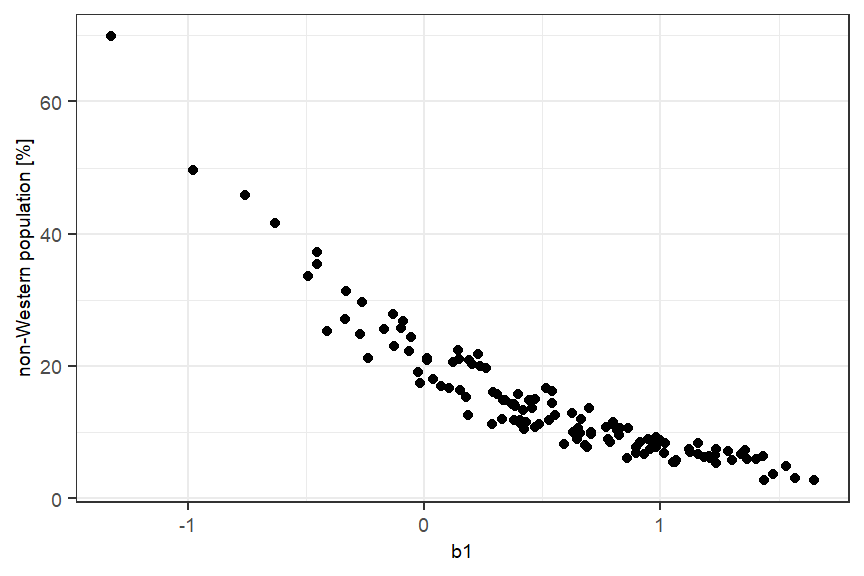
\includegraphics{CoDa_migr_cph_files/figure-latex/fig-b1-non-wst-1} 

}

\caption{Non-Western population vs. balance 1}\label{fig:fig-b1-non-wst}
\end{figure}

\hypertarget{spatial-autocorrelation-of-balances}{%
\subsubsection{Spatial autocorrelation of
balances}\label{spatial-autocorrelation-of-balances}}

Global Moran index:

\begin{Shaded}
\begin{Highlighting}[]
\CommentTok{\# Moran}
\NormalTok{nb }\OtherTok{\textless{}{-}} \FunctionTok{poly2nb}\NormalTok{(cptl\_prsh\_ancestry\_sf, }\AttributeTok{queen =} \ConstantTok{TRUE}\NormalTok{)}
\NormalTok{wts }\OtherTok{\textless{}{-}} \FunctionTok{nb2listw}\NormalTok{(nb, }\AttributeTok{style =} \StringTok{"W"}\NormalTok{, }\AttributeTok{zero.policy =} \ConstantTok{TRUE}\NormalTok{)}

\CommentTok{\# Global index}
\NormalTok{GMI\_b1 }\OtherTok{\textless{}{-}} \FunctionTok{moran.test}\NormalTok{(cptl\_prsh\_ancestry\_sf}\SpecialCharTok{$}\NormalTok{b1, }\AttributeTok{listw =}\NormalTok{ wts) }\SpecialCharTok{\%\textgreater{}\%}
  \FunctionTok{tidy}\NormalTok{() }\SpecialCharTok{\%\textgreater{}\%} 
  \FunctionTok{mutate}\NormalTok{(}\AttributeTok{balance =} \StringTok{"b1"}\NormalTok{) }\SpecialCharTok{\%\textgreater{}\%} 
  \FunctionTok{select}\NormalTok{(balance, }\FunctionTok{everything}\NormalTok{()) }\SpecialCharTok{\%\textgreater{}\%} 
  \FunctionTok{rename}\NormalTok{(}\AttributeTok{moran\_I  =}\NormalTok{ estimate1,}
         \AttributeTok{expectation =}\NormalTok{ estimate2,}
         \AttributeTok{variance =}\NormalTok{ estimate3)}

\NormalTok{GMI\_b2 }\OtherTok{\textless{}{-}} \FunctionTok{moran.test}\NormalTok{(cptl\_prsh\_ancestry\_sf}\SpecialCharTok{$}\NormalTok{b2, }\AttributeTok{listw =}\NormalTok{ wts) }\SpecialCharTok{\%\textgreater{}\%}
  \FunctionTok{tidy}\NormalTok{() }\SpecialCharTok{\%\textgreater{}\%} 
  \FunctionTok{mutate}\NormalTok{(}\AttributeTok{balance =} \StringTok{"b2"}\NormalTok{) }\SpecialCharTok{\%\textgreater{}\%} 
  \FunctionTok{select}\NormalTok{(balance, }\FunctionTok{everything}\NormalTok{()) }\SpecialCharTok{\%\textgreater{}\%} 
  \FunctionTok{rename}\NormalTok{(}\AttributeTok{moran\_I  =}\NormalTok{ estimate1,}
         \AttributeTok{expectation =}\NormalTok{ estimate2,}
         \AttributeTok{variance =}\NormalTok{ estimate3)}

\FunctionTok{bind\_rows}\NormalTok{(GMI\_b1, GMI\_b2) }\SpecialCharTok{\%\textgreater{}\%}
  \FunctionTok{kbl}\NormalTok{(}\AttributeTok{caption =} \StringTok{"Spatial autocorrelation of balances"}\NormalTok{,}
      \AttributeTok{digits =} \FunctionTok{c}\NormalTok{(}\FunctionTok{rep}\NormalTok{(}\DecValTok{3}\NormalTok{, }\DecValTok{5}\NormalTok{), }\DecValTok{32}\NormalTok{)) }\SpecialCharTok{\%\textgreater{}\%}
  \FunctionTok{kable\_styling}\NormalTok{()}
\end{Highlighting}
\end{Shaded}

\begin{table}

\caption{\label{tab:prsh-CoDa-moran-global}Spatial autocorrelation of balances}
\centering
\begin{tabular}[t]{l|r|r|r|r|r|l|l}
\hline
balance & moran\_I & expectation & variance & statistic & p.value & method & alternative\\
\hline
b1 & 0.470 & -0.008 & 0.003 & 8.563 & 5.502511e-18 & Moran I test under randomisation & greater\\
\hline
b2 & 0.542 & -0.008 & 0.003 & 9.837 & 3.915499e-23 & Moran I test under randomisation & greater\\
\hline
\end{tabular}
\end{table}

Local Moran index:

\begin{Shaded}
\begin{Highlighting}[]
\CommentTok{\# Local Moran index}

\NormalTok{f\_local\_moran }\OtherTok{\textless{}{-}} \ControlFlowTok{function}\NormalTok{(year, }
\NormalTok{                          variable, }
                          \AttributeTok{df =}\NormalTok{ cptl\_prsh\_ancestry\_sf, }
                          \AttributeTok{signif =} \FloatTok{0.15}\NormalTok{) \{ }
  
  \CommentTok{\# Polygons}
\NormalTok{  s }\OtherTok{\textless{}{-}}\NormalTok{ df }\SpecialCharTok{\%\textgreater{}\%}
    \CommentTok{\# Select}
    \FunctionTok{filter}\NormalTok{(year }\SpecialCharTok{==}\NormalTok{ \{\{ year \}\}) }\SpecialCharTok{\%\textgreater{}\%} 
    \FunctionTok{drop\_na}\NormalTok{() }\SpecialCharTok{\%\textgreater{}\%} 
    \FunctionTok{st\_sf}\NormalTok{() }
  
  \CommentTok{\# Variable}
\NormalTok{  x }\OtherTok{\textless{}{-}}\NormalTok{ s }\SpecialCharTok{\%\textgreater{}\%} 
    \CommentTok{\# Variable}
    \FunctionTok{pull}\NormalTok{( \{\{ variable \}\}) }
  
  \CommentTok{\# Plot MI}
\NormalTok{  xp }\OtherTok{\textless{}{-}}\NormalTok{ x }\SpecialCharTok{\%\textgreater{}\%} 
    \CommentTok{\# Local Index}
    \FunctionTok{localmoran\_perm}\NormalTok{(}\AttributeTok{listw =} \FunctionTok{nb2listw}\NormalTok{(}\FunctionTok{poly2nb}\NormalTok{(s, }\AttributeTok{queen =} \ConstantTok{TRUE}\NormalTok{),}
                                     \AttributeTok{style =} \StringTok{"W"}\NormalTok{,}
                                     \AttributeTok{zero.policy =} \ConstantTok{TRUE}\NormalTok{),}
                    \AttributeTok{nsim =} \DecValTok{999}\NormalTok{) }\SpecialCharTok{\%\textgreater{}\%} 
    \FunctionTok{as\_tibble}\NormalTok{() }\SpecialCharTok{\%\textgreater{}\%} 
\NormalTok{    dplyr}\SpecialCharTok{::}\FunctionTok{rename}\NormalTok{(}\AttributeTok{p.value =} \StringTok{\textasciigrave{}}\AttributeTok{Pr(z \textgreater{} 0)}\StringTok{\textasciigrave{}}\NormalTok{) }\SpecialCharTok{\%\textgreater{}\%} 
    \CommentTok{\# binds results to our polygon shapefile}
    \FunctionTok{cbind}\NormalTok{(s) }\SpecialCharTok{\%\textgreater{}\%} 
    \FunctionTok{st\_sf}\NormalTok{() }\SpecialCharTok{\%\textgreater{}\%} 
    \CommentTok{\# center the variable of interest around its mean}
    \FunctionTok{mutate}\NormalTok{(}\AttributeTok{m\_qualification =}\NormalTok{ x }\SpecialCharTok{{-}} \FunctionTok{mean}\NormalTok{( x ),}
           \AttributeTok{m\_local =}\NormalTok{ Ii }\SpecialCharTok{{-}} \FunctionTok{mean}\NormalTok{(Ii)) }\SpecialCharTok{\%\textgreater{}\%} 
    \CommentTok{\# Build quadrant}
    \FunctionTok{mutate}\NormalTok{(}\AttributeTok{quadrant =} \FunctionTok{case\_when}\NormalTok{(m\_qualification }\SpecialCharTok{\textgreater{}} \DecValTok{0} \SpecialCharTok{\&}\NormalTok{ m\_local }\SpecialCharTok{\textgreater{}} \DecValTok{0} \SpecialCharTok{\textasciitilde{}} \DecValTok{4}\NormalTok{,}
\NormalTok{                                m\_qualification }\SpecialCharTok{\textless{}} \DecValTok{0} \SpecialCharTok{\&}\NormalTok{ m\_local }\SpecialCharTok{\textless{}} \DecValTok{0} \SpecialCharTok{\textasciitilde{}} \DecValTok{1}\NormalTok{,}
\NormalTok{                                m\_qualification }\SpecialCharTok{\textless{}} \DecValTok{0} \SpecialCharTok{\&}\NormalTok{ m\_local }\SpecialCharTok{\textgreater{}} \DecValTok{0} \SpecialCharTok{\textasciitilde{}} \DecValTok{2}\NormalTok{,}
\NormalTok{                                m\_qualification }\SpecialCharTok{\textgreater{}} \DecValTok{0} \SpecialCharTok{\&}\NormalTok{ m\_local }\SpecialCharTok{\textless{}} \DecValTok{0} \SpecialCharTok{\textasciitilde{}} \DecValTok{3}\NormalTok{),}
           \AttributeTok{quadrant =} \FunctionTok{ifelse}\NormalTok{(p.value }\SpecialCharTok{\textgreater{}}\NormalTok{ signif, }\DecValTok{0}\NormalTok{, quadrant)) }\SpecialCharTok{\%\textgreater{}\%} 
    \FunctionTok{mutate}\NormalTok{(}\AttributeTok{quadrant =} \FunctionTok{factor}\NormalTok{(quadrant,}
                             \AttributeTok{levels =} \FunctionTok{c}\NormalTok{(}\DecValTok{0}\NormalTok{, }\DecValTok{1}\NormalTok{, }\DecValTok{2}\NormalTok{, }\DecValTok{3}\NormalTok{, }\DecValTok{4}\NormalTok{), }
                             \AttributeTok{labels =}  \FunctionTok{c}\NormalTok{(}\StringTok{"Insignificant"}\NormalTok{,}
                                         \StringTok{"Low{-}Low"}\NormalTok{,}
                                         \StringTok{"Low{-}High"}\NormalTok{,}
                                         \StringTok{"High{-}Low"}\NormalTok{,}
                                         \StringTok{"High{-}High"}\NormalTok{))) }
  
\NormalTok{  xp }\SpecialCharTok{\%\textgreater{}\%} 
    \CommentTok{\# Plot quadrants (LISA)}
    \FunctionTok{ggplot}\NormalTok{() }\SpecialCharTok{+}
    \FunctionTok{geom\_sf}\NormalTok{(}\AttributeTok{data =}\NormalTok{ dk\_country\_crop, }\AttributeTok{fill =} \StringTok{"grey"}\NormalTok{) }\SpecialCharTok{+}
    \FunctionTok{geom\_sf}\NormalTok{(}\FunctionTok{aes}\NormalTok{(}\AttributeTok{fill =}\NormalTok{ quadrant), }\AttributeTok{color =} \StringTok{"grey"}\NormalTok{, }\AttributeTok{size =} \FloatTok{0.05}\NormalTok{) }\SpecialCharTok{+}
    \FunctionTok{geom\_sf}\NormalTok{(}\AttributeTok{data =}\NormalTok{ cptl\_muni, }\AttributeTok{fill =} \ConstantTok{NA}\NormalTok{, }\AttributeTok{color =} \StringTok{"white"}\NormalTok{, }\AttributeTok{size =} \FloatTok{0.5}\NormalTok{) }\SpecialCharTok{+} 
    \FunctionTok{scale\_fill\_manual}\NormalTok{(}\AttributeTok{name =} \StringTok{"Quadrant"}\NormalTok{ ,}
                      \AttributeTok{values =} \FunctionTok{c}\NormalTok{(}\StringTok{"lightgrey"}\NormalTok{,}
                                 \StringTok{"\#0000FF"}\NormalTok{,}
                                 \StringTok{"\#A2A2FF"}\NormalTok{,}
                                 \StringTok{"\#FFA2A2"}\NormalTok{,}
                                 \StringTok{"\#FF0000"}\NormalTok{),}
                      \AttributeTok{drop =} \ConstantTok{FALSE}\NormalTok{) }\SpecialCharTok{+}
    \FunctionTok{labs}\NormalTok{(}\AttributeTok{title =}\NormalTok{ \{\{ variable \}\}) }\SpecialCharTok{+}
    \FunctionTok{theme\_void}\NormalTok{()}
  
\NormalTok{\}}
\end{Highlighting}
\end{Shaded}

\begin{Shaded}
\begin{Highlighting}[]
\NormalTok{p1 }\OtherTok{\textless{}{-}} \FunctionTok{f\_local\_moran}\NormalTok{(}\AttributeTok{df =}\NormalTok{ cptl\_prsh\_ancestry\_sf,}
              \AttributeTok{year =} \DecValTok{2020}\NormalTok{, }
              \AttributeTok{variable =} \StringTok{"b1"}\NormalTok{, }
              \AttributeTok{signif =} \FloatTok{0.1}\NormalTok{)}

\NormalTok{p2 }\OtherTok{\textless{}{-}} \FunctionTok{f\_local\_moran}\NormalTok{(}\AttributeTok{df =}\NormalTok{ cptl\_prsh\_ancestry\_sf,}
              \AttributeTok{year =} \DecValTok{2020}\NormalTok{, }
              \AttributeTok{variable =} \StringTok{"b2"}\NormalTok{, }
              \AttributeTok{signif =} \FloatTok{0.1}\NormalTok{)}

\NormalTok{p1 }\SpecialCharTok{+}\NormalTok{ p2 }\SpecialCharTok{+} \FunctionTok{plot\_layout}\NormalTok{(}\AttributeTok{guides =} \StringTok{"collect"}\NormalTok{)}
\end{Highlighting}
\end{Shaded}

\begin{figure}[H]

{\centering 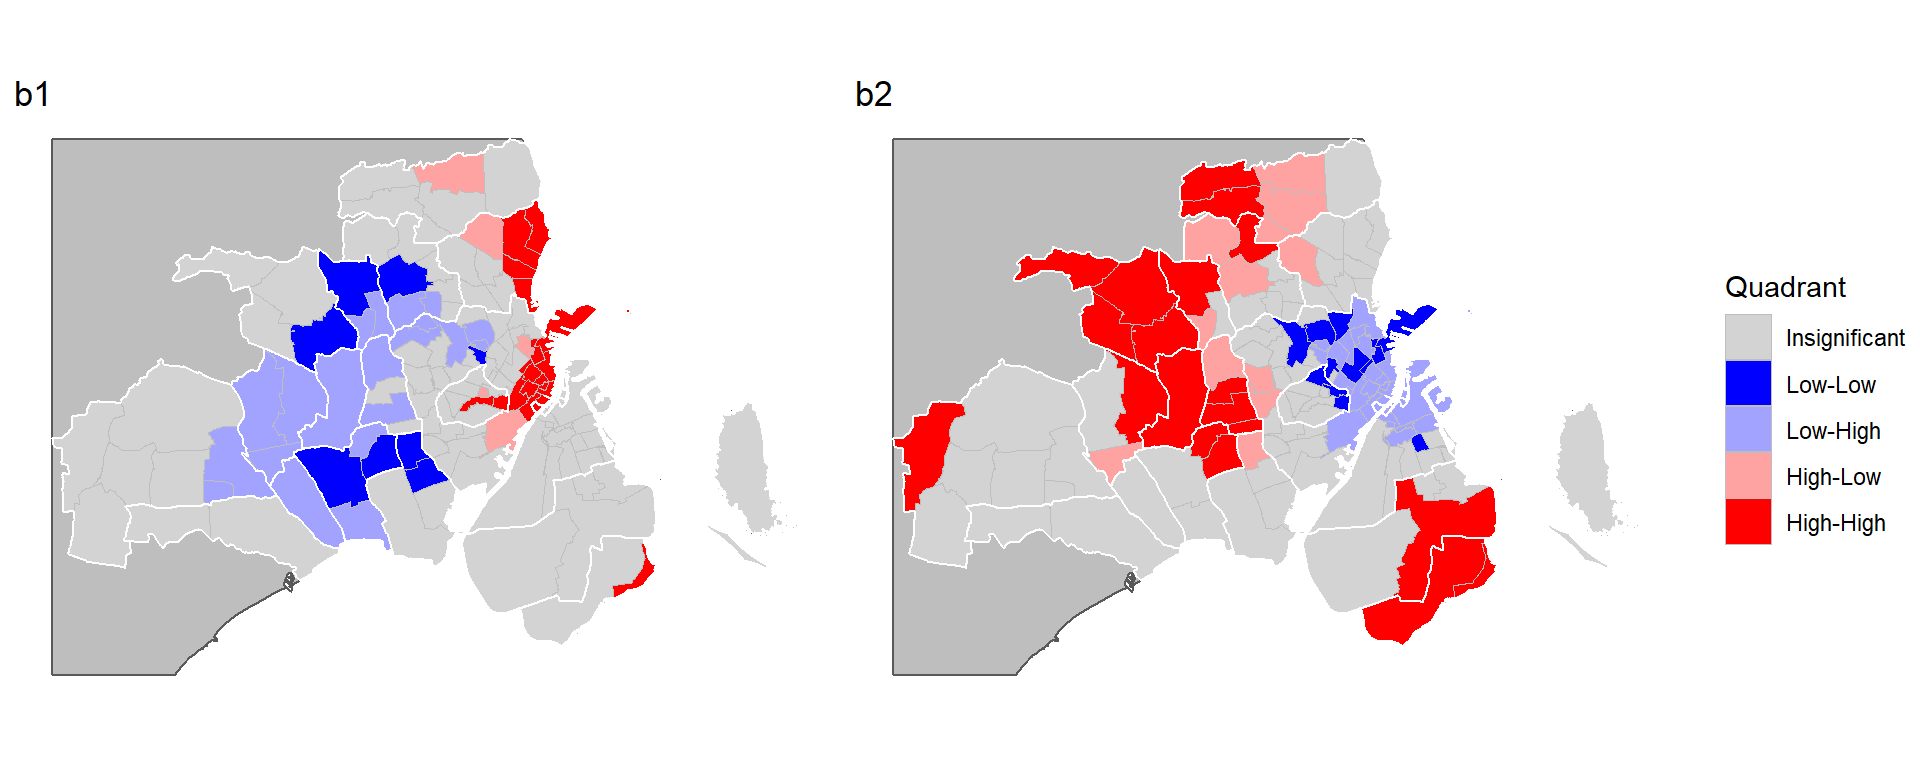
\includegraphics{CoDa_migr_cph_files/figure-latex/fig-local-moran-balances-1} 

}

\caption{LISA plot for each balance}\label{fig:fig-local-moran-balances}
\end{figure}

\hypertarget{hierarchical-cluster}{%
\subsubsection{Hierarchical cluster:}\label{hierarchical-cluster}}

\begin{Shaded}
\begin{Highlighting}[]
\CommentTok{\# Dissimilarity matrix}
\NormalTok{d }\OtherTok{\textless{}{-}}\NormalTok{ cptl\_prsh\_ancestry\_sf }\SpecialCharTok{\%\textgreater{}\%} 
  \FunctionTok{select}\NormalTok{(b1, b2) }\SpecialCharTok{\%\textgreater{}\%} 
  \FunctionTok{as\_tibble}\NormalTok{() }\SpecialCharTok{\%\textgreater{}\%} 
  \FunctionTok{select}\NormalTok{(}\SpecialCharTok{{-}}\NormalTok{geometry) }\SpecialCharTok{\%\textgreater{}\%} 
  \FunctionTok{scale}\NormalTok{() }\SpecialCharTok{\%\textgreater{}\%} 
  \FunctionTok{dist}\NormalTok{(}\AttributeTok{method =} \StringTok{"euclidean"}\NormalTok{)}

\CommentTok{\# Hierarchical clustering}
\NormalTok{hcl }\OtherTok{\textless{}{-}} \FunctionTok{hclust}\NormalTok{(d, }\AttributeTok{method =} \StringTok{"ward.D2"}\NormalTok{)}

\CommentTok{\# Add four Clusters}
\NormalTok{cptl\_prsh\_ancestry\_sf }\OtherTok{\textless{}{-}}\NormalTok{ cptl\_prsh\_ancestry\_sf }\SpecialCharTok{\%\textgreater{}\%}
  \FunctionTok{mutate}\NormalTok{(}\AttributeTok{CL2 =} \FunctionTok{cutree}\NormalTok{(hcl, }\AttributeTok{k =} \DecValTok{2}\NormalTok{),}
         \AttributeTok{CL3 =} \FunctionTok{cutree}\NormalTok{(hcl, }\AttributeTok{k =} \DecValTok{3}\NormalTok{),}
         \AttributeTok{CL4 =} \FunctionTok{cutree}\NormalTok{(hcl, }\AttributeTok{k =} \DecValTok{4}\NormalTok{)) }\SpecialCharTok{\%\textgreater{}\%} 
  \FunctionTok{mutate}\NormalTok{(}\FunctionTok{across}\NormalTok{(}\AttributeTok{.cols =} \FunctionTok{c}\NormalTok{(CL2, CL3, CL4), }\AttributeTok{.fns =}\NormalTok{ factor))}
\end{Highlighting}
\end{Shaded}

\begin{Shaded}
\begin{Highlighting}[]
\CommentTok{\# Plot}
\FunctionTok{plot}\NormalTok{(hcl, }\AttributeTok{hang =} \SpecialCharTok{{-}}\DecValTok{1}\NormalTok{, }\AttributeTok{cex =} \FloatTok{0.4}\NormalTok{, }\AttributeTok{xlab =} \StringTok{"Parish ID"}\NormalTok{)}
\FunctionTok{rect.hclust}\NormalTok{(hcl, }\AttributeTok{k =} \DecValTok{2}\NormalTok{, }\AttributeTok{border =} \StringTok{"\#0072B2"}\NormalTok{)}
\FunctionTok{rect.hclust}\NormalTok{(hcl, }\AttributeTok{k =} \DecValTok{4}\NormalTok{, }\AttributeTok{border =} \StringTok{"\#D55E00"}\NormalTok{)}
\end{Highlighting}
\end{Shaded}

\begin{figure}[H]

{\centering 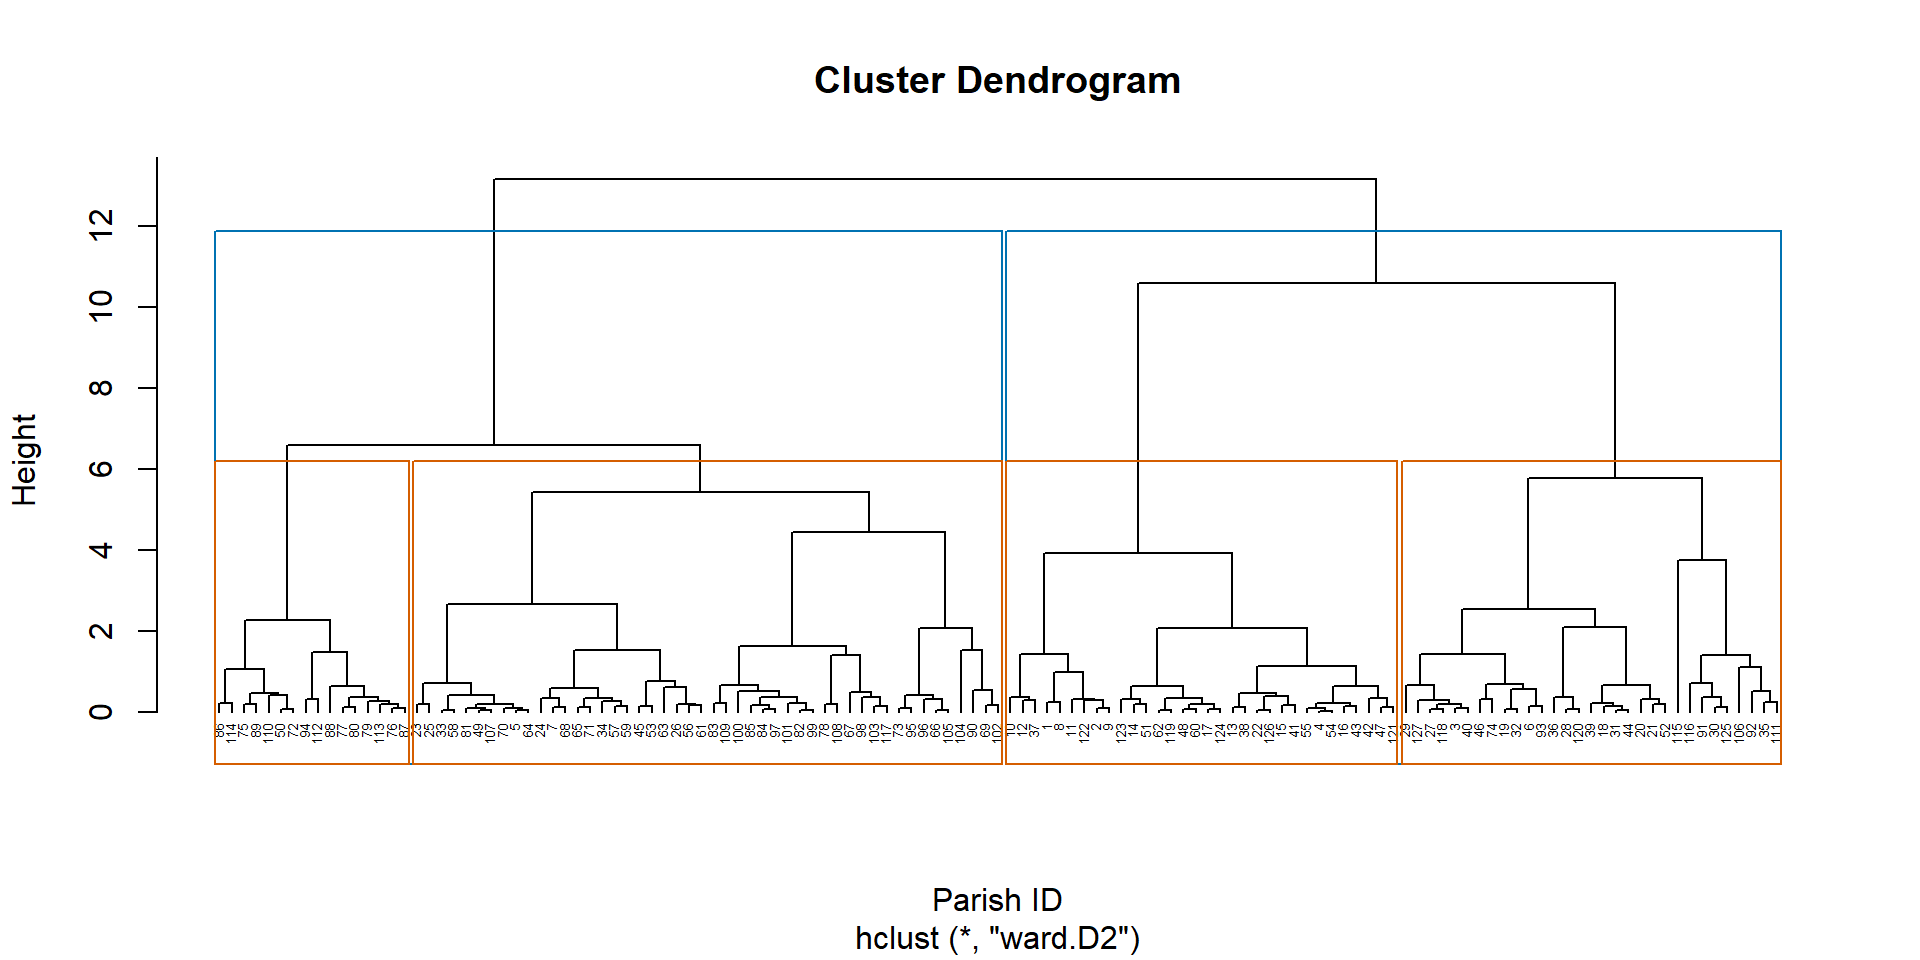
\includegraphics{CoDa_migr_cph_files/figure-latex/fig-prsh-CoDa-cluster-1} 

}

\caption{Cluster dendrogram}\label{fig:fig-prsh-CoDa-cluster}
\end{figure}

\begin{Shaded}
\begin{Highlighting}[]
\NormalTok{pCL2 }\OtherTok{\textless{}{-}}\NormalTok{ cptl\_prsh\_ancestry\_sf }\SpecialCharTok{\%\textgreater{}\%} 
  \FunctionTok{ggplot}\NormalTok{() }\SpecialCharTok{+}
  \FunctionTok{geom\_sf}\NormalTok{(}\AttributeTok{data =}\NormalTok{ dk\_country\_crop, }\AttributeTok{fill =} \StringTok{"grey"}\NormalTok{) }\SpecialCharTok{+}
  \FunctionTok{geom\_sf}\NormalTok{(}\FunctionTok{aes}\NormalTok{(}\AttributeTok{fill =}\NormalTok{ CL2)) }\SpecialCharTok{+}
  \FunctionTok{geom\_sf}\NormalTok{(}\AttributeTok{data =}\NormalTok{ cptl\_muni, }\AttributeTok{fill =} \ConstantTok{NA}\NormalTok{, }\AttributeTok{color =} \StringTok{"white"}\NormalTok{, }\AttributeTok{size =} \FloatTok{0.5}\NormalTok{) }\SpecialCharTok{+}
  \FunctionTok{scale\_fill\_manual}\NormalTok{(}\AttributeTok{name =} \StringTok{"Cluster"}\NormalTok{,}
                    \AttributeTok{values =} \FunctionTok{c}\NormalTok{(}\StringTok{"\#542788"}\NormalTok{,}
                               \StringTok{"\#B35806"}\NormalTok{)) }\SpecialCharTok{+}
  \FunctionTok{geom\_sf}\NormalTok{(}\AttributeTok{data =}\NormalTok{ cptl\_muni, }\AttributeTok{fill =} \ConstantTok{NA}\NormalTok{, }\AttributeTok{color =} \StringTok{"white"}\NormalTok{, }\AttributeTok{size =} \FloatTok{0.5}\NormalTok{) }\SpecialCharTok{+}
  \FunctionTok{theme\_void}\NormalTok{()}

\NormalTok{pCL3 }\OtherTok{\textless{}{-}}\NormalTok{ cptl\_prsh\_ancestry\_sf }\SpecialCharTok{\%\textgreater{}\%} 
  \FunctionTok{ggplot}\NormalTok{() }\SpecialCharTok{+}
  \FunctionTok{geom\_sf}\NormalTok{(}\AttributeTok{data =}\NormalTok{ dk\_country\_crop, }\AttributeTok{fill =} \StringTok{"grey"}\NormalTok{) }\SpecialCharTok{+}
  \FunctionTok{geom\_sf}\NormalTok{(}\FunctionTok{aes}\NormalTok{(}\AttributeTok{fill =}\NormalTok{ CL3)) }\SpecialCharTok{+}
  \FunctionTok{geom\_sf}\NormalTok{(}\AttributeTok{data =}\NormalTok{ cptl\_muni, }\AttributeTok{fill =} \ConstantTok{NA}\NormalTok{, }\AttributeTok{color =} \StringTok{"white"}\NormalTok{, }\AttributeTok{size =} \FloatTok{0.5}\NormalTok{) }\SpecialCharTok{+}
  \FunctionTok{scale\_fill\_manual}\NormalTok{(}\AttributeTok{name =} \StringTok{"Cluster"}\NormalTok{,}
                    \AttributeTok{values =} \FunctionTok{c}\NormalTok{(}\StringTok{"\#998EC3"}\NormalTok{,}
                               \StringTok{"\#D8DAEB"}\NormalTok{,}
                               \StringTok{"\#B35806"}\NormalTok{)) }\SpecialCharTok{+}
  \FunctionTok{geom\_sf}\NormalTok{(}\AttributeTok{data =}\NormalTok{ cptl\_muni, }\AttributeTok{fill =} \ConstantTok{NA}\NormalTok{, }\AttributeTok{color =} \StringTok{"white"}\NormalTok{, }\AttributeTok{size =} \FloatTok{0.5}\NormalTok{) }\SpecialCharTok{+}
  \FunctionTok{theme\_void}\NormalTok{()}

\NormalTok{pCL4 }\OtherTok{\textless{}{-}}\NormalTok{ cptl\_prsh\_ancestry\_sf }\SpecialCharTok{\%\textgreater{}\%} 
  \FunctionTok{ggplot}\NormalTok{() }\SpecialCharTok{+}
  \FunctionTok{geom\_sf}\NormalTok{(}\AttributeTok{data =}\NormalTok{ dk\_country\_crop, }\AttributeTok{fill =} \StringTok{"grey"}\NormalTok{) }\SpecialCharTok{+}
  \FunctionTok{geom\_sf}\NormalTok{(}\FunctionTok{aes}\NormalTok{(}\AttributeTok{fill =}\NormalTok{ CL4)) }\SpecialCharTok{+}
  \FunctionTok{geom\_sf}\NormalTok{(}\AttributeTok{data =}\NormalTok{ cptl\_muni, }\AttributeTok{fill =} \ConstantTok{NA}\NormalTok{, }\AttributeTok{color =} \StringTok{"white"}\NormalTok{, }\AttributeTok{size =} \FloatTok{0.5}\NormalTok{) }\SpecialCharTok{+}
  \FunctionTok{scale\_fill\_manual}\NormalTok{(}\AttributeTok{name =} \StringTok{"Cluster"}\NormalTok{,}
                    \AttributeTok{values =} \FunctionTok{c}\NormalTok{(}\StringTok{"\#998EC3"}\NormalTok{,}
                               \StringTok{"\#D8DAEB"}\NormalTok{,}
                               \StringTok{"\#F1A340"}\NormalTok{,}
                               \StringTok{"\#FEE0B6"}\NormalTok{)) }\SpecialCharTok{+}
  \FunctionTok{geom\_sf}\NormalTok{(}\AttributeTok{data =}\NormalTok{ cptl\_muni, }\AttributeTok{fill =} \ConstantTok{NA}\NormalTok{, }\AttributeTok{color =} \StringTok{"white"}\NormalTok{, }\AttributeTok{size =} \FloatTok{0.5}\NormalTok{) }\SpecialCharTok{+}
  \FunctionTok{theme\_void}\NormalTok{()}
 
\NormalTok{pCL4}
\end{Highlighting}
\end{Shaded}

\begin{figure}[H]

{\centering 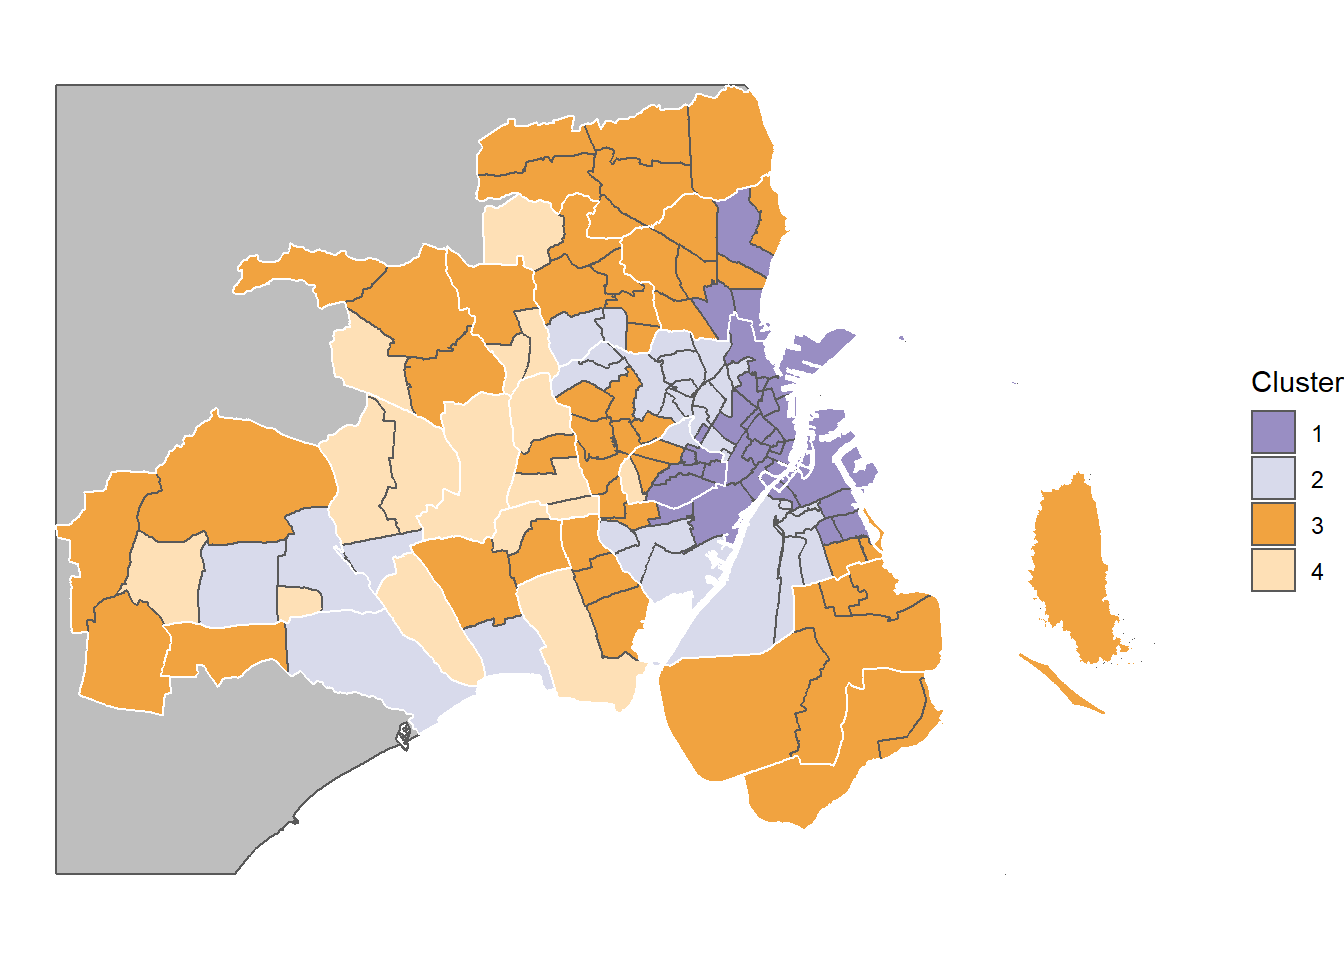
\includegraphics{CoDa_migr_cph_files/figure-latex/fig-prsh-CoDa-cluster-k4-1} 

}

\caption{Clusters based on balances (b1 amd b2)}\label{fig:fig-prsh-CoDa-cluster-k4}
\end{figure}

Compositional means of the clusters:

\begin{Shaded}
\begin{Highlighting}[]
\NormalTok{CL4\_comp\_means }\OtherTok{\textless{}{-}}\NormalTok{ cptl\_prsh\_ancestry\_sf }\SpecialCharTok{\%\textgreater{}\%} 
  \FunctionTok{as\_tibble}\NormalTok{() }\SpecialCharTok{\%\textgreater{}\%} 
  \FunctionTok{select}\NormalTok{(CL4, pop\_dan\_pct,  pop\_frgn\_wst\_pct,   pop\_frgn\_nwst\_pct,  }\SpecialCharTok{{-}}\NormalTok{geometry) }\SpecialCharTok{\%\textgreater{}\%}
  \FunctionTok{group\_split}\NormalTok{(CL4, }\AttributeTok{.keep =} \ConstantTok{FALSE}\NormalTok{) }\SpecialCharTok{\%\textgreater{}\%}
  \FunctionTok{map}\NormalTok{(., }\SpecialCharTok{\textasciitilde{}}\FunctionTok{alr}\NormalTok{(.)) }\SpecialCharTok{\%\textgreater{}\%}
  \FunctionTok{map}\NormalTok{(., }\SpecialCharTok{\textasciitilde{}}\FunctionTok{mean}\NormalTok{(.)) }\SpecialCharTok{\%\textgreater{}\%} 
  \FunctionTok{map\_dfr}\NormalTok{(., }\SpecialCharTok{\textasciitilde{}}\FunctionTok{alrInv}\NormalTok{(.)) }\SpecialCharTok{\%\textgreater{}\%} 
  \FunctionTok{mutate}\NormalTok{(}\AttributeTok{CL4 =} \FunctionTok{factor}\NormalTok{(}\FunctionTok{c}\NormalTok{(}\DecValTok{1}\NormalTok{, }\DecValTok{2}\NormalTok{, }\DecValTok{3}\NormalTok{, }\DecValTok{4}\NormalTok{))) }\SpecialCharTok{\%\textgreater{}\%} 
  \FunctionTok{select}\NormalTok{(CL4, }\FunctionTok{everything}\NormalTok{()) }\SpecialCharTok{\%\textgreater{}\%} 
  \FunctionTok{mutate}\NormalTok{(}\FunctionTok{across}\NormalTok{(}\FunctionTok{where}\NormalTok{(is.numeric), }\SpecialCharTok{\textasciitilde{}}\NormalTok{ .x }\SpecialCharTok{*} \DecValTok{100}\NormalTok{))}

\NormalTok{CL4\_comp\_means }\SpecialCharTok{\%\textgreater{}\%} 
  \FunctionTok{kbl}\NormalTok{(}\AttributeTok{caption =} \StringTok{"Compositional means of the clusters"}\NormalTok{,}
      \AttributeTok{col.names =} \FunctionTok{c}\NormalTok{(}\StringTok{"Cluster"}\NormalTok{, }\StringTok{"Danes"}\NormalTok{, }\StringTok{"Western"}\NormalTok{, }\StringTok{"Non{-}Western"}\NormalTok{), }
      \AttributeTok{digits =} \DecValTok{1}\NormalTok{) }\SpecialCharTok{\%\textgreater{}\%}
  \FunctionTok{kable\_styling}\NormalTok{()}
\end{Highlighting}
\end{Shaded}

\begin{table}

\caption{\label{tab:comp-mean}Compositional means of the clusters}
\centering
\begin{tabular}[t]{l|r|r|r}
\hline
Cluster & Danes & Western & Non-Western\\
\hline
1 & 81.0 & 11.2 & 7.8\\
\hline
2 & 66.6 & 9.3 & 24.1\\
\hline
3 & 85.9 & 5.2 & 8.9\\
\hline
4 & 74.8 & 4.7 & 20.5\\
\hline
\end{tabular}
\end{table}

Population statistics (in percentage) by clusters (k = 4):

\begin{Shaded}
\begin{Highlighting}[]
\CommentTok{\# Create variable labels of the variables to be printed in the table}
\NormalTok{labelled}\SpecialCharTok{::}\FunctionTok{var\_label}\NormalTok{(cptl\_prsh\_ancestry\_sf}\SpecialCharTok{$}\NormalTok{pop\_dan\_pct)       }\OtherTok{\textless{}{-}} \StringTok{"Danes"}
\NormalTok{labelled}\SpecialCharTok{::}\FunctionTok{var\_label}\NormalTok{(cptl\_prsh\_ancestry\_sf}\SpecialCharTok{$}\NormalTok{pop\_frgn\_wst\_pct)  }\OtherTok{\textless{}{-}} \StringTok{"Western"}
\NormalTok{labelled}\SpecialCharTok{::}\FunctionTok{var\_label}\NormalTok{(cptl\_prsh\_ancestry\_sf}\SpecialCharTok{$}\NormalTok{pop\_frgn\_nwst\_pct) }\OtherTok{\textless{}{-}} \StringTok{"Non{-}Western"}

\CommentTok{\# table}
\NormalTok{cptl\_prsh\_ancestry\_sf }\SpecialCharTok{\%\textgreater{}\%} 
  \FunctionTok{as\_tibble}\NormalTok{() }\SpecialCharTok{\%\textgreater{}\%} 
  \FunctionTok{select}\NormalTok{(CL4, pop\_dan\_pct,  pop\_frgn\_wst\_pct,   pop\_frgn\_nwst\_pct,  }\SpecialCharTok{{-}}\NormalTok{geometry) }\SpecialCharTok{\%\textgreater{}\%} 
  \FunctionTok{tbl\_summary}\NormalTok{(}\AttributeTok{by =}\NormalTok{ CL4,}
              \AttributeTok{type =} \FunctionTok{all\_continuous}\NormalTok{() }\SpecialCharTok{\textasciitilde{}} \StringTok{"continuous2"}\NormalTok{,}
              \AttributeTok{statistic =} \FunctionTok{all\_continuous}\NormalTok{() }\SpecialCharTok{\textasciitilde{}} \FunctionTok{c}\NormalTok{(}\StringTok{"\{mean\}"}\NormalTok{,}
                                               \StringTok{"\{median\}"}\NormalTok{,}
                                               \StringTok{"\{p25\} {-} \{p75\}"}\NormalTok{,}
                                               \StringTok{"\{min\} {-} \{max\}"}\NormalTok{),}
              \AttributeTok{missing =} \StringTok{"no"}\NormalTok{,}
              \AttributeTok{digits =} \FunctionTok{all\_continuous}\NormalTok{() }\SpecialCharTok{\textasciitilde{}} \DecValTok{1}\NormalTok{) }\SpecialCharTok{\%\textgreater{}\%}
  \FunctionTok{bold\_labels}\NormalTok{()}
\end{Highlighting}
\end{Shaded}

\begin{tabular}{l|l|l|l|l}
\hline
**Characteristic** & **1**, N = 32 & **2**, N = 31 & **3**, N = 48 & **4**, N = 16\\
\hline
\_\_Danes\_\_ &  &  &  & \\
\hline
Mean & 80.6 & 65.3 & 85.1 & 74.5\\
\hline
Median & 81.1 & 69.2 & 84.6 & 74.1\\
\hline
IQR & 78.4 - 82.9 & 62.3 - 71.8 & 83.1 - 88.3 & 71.7 - 78.6\\
\hline
Range & 72.9 - 85.6 & 21.2 - 78.7 & 77.3 - 94.6 & 68.0 - 80.3\\
\hline
\_\_Western\_\_ &  &  &  & \\
\hline
Mean & 11.5 & 9.2 & 5.3 & 4.8\\
\hline
Median & 10.4 & 8.9 & 5.5 & 4.6\\
\hline
IQR & 9.5 - 12.3 & 7.7 - 10.1 & 4.4 - 6.4 & 4.4 - 5.5\\
\hline
Range & 8.3 - 19.9 & 4.9 - 14.2 & 2.7 - 7.9 & 3.2 - 6.4\\
\hline
\_\_Non-Western\_\_ &  &  &  & \\
\hline
Mean & 7.9 & 25.5 & 9.6 & 20.7\\
\hline
Median & 7.4 & 21.0 & 9.9 & 21.1\\
\hline
IQR & 6.4 - 9.0 & 16.0 - 30.5 & 7.3 - 11.9 & 17.3 - 23.4\\
\hline
Range & 4.9 - 11.6 & 12.0 - 69.9 & 2.7 - 16.0 & 15.2 - 27.2\\
\hline
\end{tabular}

Box-plot:

\begin{Shaded}
\begin{Highlighting}[]
\NormalTok{cptl\_prsh\_ancestry\_sf }\SpecialCharTok{\%\textgreater{}\%} 
  \FunctionTok{select}\NormalTok{(CL4, pop\_dan\_pct, pop\_frgn\_nwst\_pct, pop\_frgn\_wst\_pct) }\SpecialCharTok{\%\textgreater{}\%}
  \FunctionTok{as\_tibble}\NormalTok{() }\SpecialCharTok{\%\textgreater{}\%}
  \FunctionTok{pivot\_longer}\NormalTok{(}\SpecialCharTok{!}\FunctionTok{c}\NormalTok{(CL4, geometry),}
               \AttributeTok{names\_to =} \StringTok{"name"}\NormalTok{, }
               \AttributeTok{values\_to =} \StringTok{"value"}\NormalTok{) }\SpecialCharTok{\%\textgreater{}\%}
  \FunctionTok{mutate}\NormalTok{(}\AttributeTok{name =} \FunctionTok{gsub}\NormalTok{(}\StringTok{"pop\_"}\NormalTok{, }\StringTok{""}\NormalTok{, name),}
         \AttributeTok{name =} \FunctionTok{gsub}\NormalTok{(}\StringTok{"\_pct"}\NormalTok{, }\StringTok{""}\NormalTok{, name),}
         \AttributeTok{name =} \FunctionTok{gsub}\NormalTok{(}\StringTok{"frgn\_"}\NormalTok{, }\StringTok{""}\NormalTok{, name))  }\SpecialCharTok{\%\textgreater{}\%}
  \FunctionTok{ggplot}\NormalTok{() }\SpecialCharTok{+} 
  \FunctionTok{geom\_boxplot}\NormalTok{(}\FunctionTok{aes}\NormalTok{(}\AttributeTok{y =}\NormalTok{ value, }\AttributeTok{x =}\NormalTok{ name, }\AttributeTok{fill =}\NormalTok{ CL4)) }\SpecialCharTok{+}
  \FunctionTok{scale\_fill\_manual}\NormalTok{(}\AttributeTok{name =} \StringTok{"Cluster"}\NormalTok{,}
                    \AttributeTok{values =} \FunctionTok{c}\NormalTok{(}\StringTok{"\#998EC3"}\NormalTok{,}
                               \StringTok{"\#D8DAEB"}\NormalTok{,}
                               \StringTok{"\#F1A340"}\NormalTok{,}
                               \StringTok{"\#FEE0B6"}\NormalTok{)) }\SpecialCharTok{+}
  \FunctionTok{labs}\NormalTok{(}\AttributeTok{x =} \StringTok{""}\NormalTok{,}
       \AttributeTok{y =} \StringTok{"Percentage [\%]"}\NormalTok{)  }\SpecialCharTok{+}
  \FunctionTok{theme}\NormalTok{(}\AttributeTok{legend.position =} \StringTok{"none"}\NormalTok{) }\SpecialCharTok{+}
  \FunctionTok{facet\_grid}\NormalTok{(}\SpecialCharTok{\textasciitilde{}}\NormalTok{CL4) }
\end{Highlighting}
\end{Shaded}

\begin{figure}[H]

{\centering 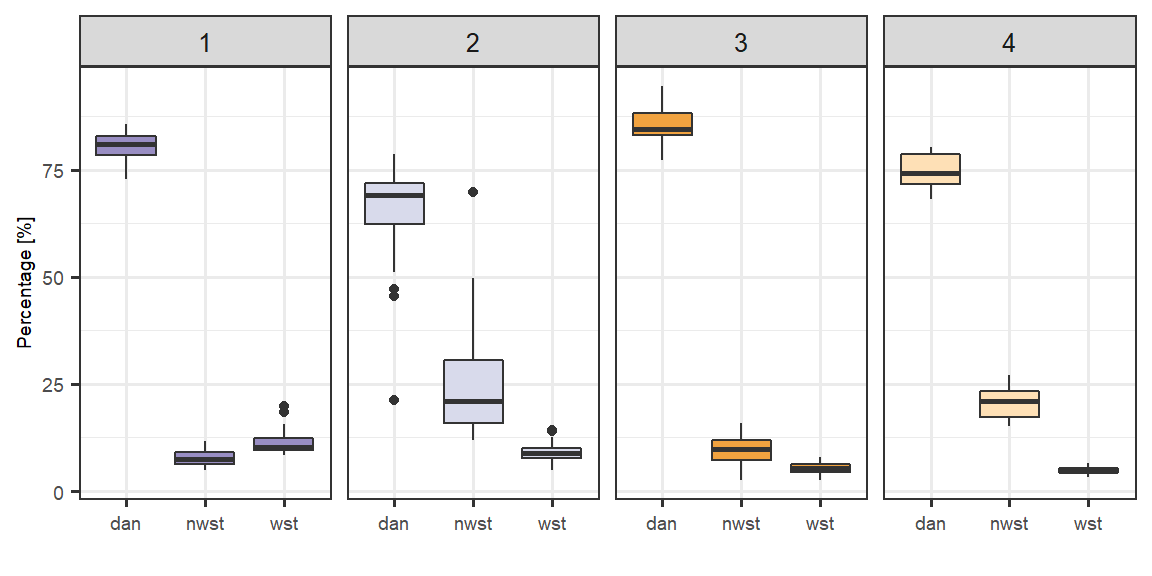
\includegraphics{CoDa_migr_cph_files/figure-latex/fig-prsh-CoDa-cluster-boxplot-1} 

}

\caption{Boxplots of the population structure in each cluster}\label{fig:fig-prsh-CoDa-cluster-boxplot}
\end{figure}

Cluster (k = 4) vs.~house prices:

\begin{Shaded}
\begin{Highlighting}[]
\NormalTok{sum\_runits\_oft\_prices }\OtherTok{\textless{}{-}} \FunctionTok{as\_tibble}\NormalTok{(sum\_runits\_oft\_prices) }\SpecialCharTok{\%\textgreater{}\%}
  \CommentTok{\# Add balances and clusters }
  \FunctionTok{left\_join}\NormalTok{(}\FunctionTok{as\_tibble}\NormalTok{(cptl\_prsh\_ancestry\_sf)) }\SpecialCharTok{\%\textgreater{}\%} 
  \FunctionTok{droplevels}\NormalTok{() }

\NormalTok{sum\_runits\_oft\_prices }\SpecialCharTok{\%\textgreater{}\%} 
  \FunctionTok{select}\NormalTok{(CL4, mean\_kDKK\_m2, median\_kDKK\_m2, }\SpecialCharTok{{-}}\NormalTok{geometry) }\SpecialCharTok{\%\textgreater{}\%} 
  \FunctionTok{tbl\_summary}\NormalTok{(}\AttributeTok{by =}\NormalTok{ CL4,}
              \AttributeTok{type =} \FunctionTok{all\_continuous}\NormalTok{() }\SpecialCharTok{\textasciitilde{}} \StringTok{"continuous2"}\NormalTok{,}
              \AttributeTok{statistic =} \FunctionTok{all\_continuous}\NormalTok{() }\SpecialCharTok{\textasciitilde{}} \FunctionTok{c}\NormalTok{(}\StringTok{"\{mean\}"}\NormalTok{,}
                                               \StringTok{"\{median\}"}\NormalTok{,}
                                               \StringTok{"\{p25\} {-} \{p75\}"}\NormalTok{,}
                                               \StringTok{"\{min\} {-} \{max\}"}\NormalTok{),}
              \AttributeTok{missing =} \StringTok{"no"}\NormalTok{,}
              \AttributeTok{digits =} \FunctionTok{all\_continuous}\NormalTok{() }\SpecialCharTok{\textasciitilde{}} \DecValTok{1}\NormalTok{) }\SpecialCharTok{\%\textgreater{}\%}
  \FunctionTok{bold\_labels}\NormalTok{()}
\end{Highlighting}
\end{Shaded}

\begin{tabular}{l|l|l|l|l}
\hline
**Characteristic** & **1**, N = 32 & **2**, N = 29 & **3**, N = 48 & **4**, N = 16\\
\hline
\_\_Mean (kDKK/m2)\_\_ &  &  &  & \\
\hline
Mean & 119.8 & 82.9 & 65.7 & 59.9\\
\hline
Median & 57.0 & 41.7 & 38.2 & 27.2\\
\hline
IQR & 50.7 - 98.7 & 37.3 - 60.8 & 31.4 - 49.8 & 24.8 - 33.5\\
\hline
Range & 39.4 - 1,132.9 & 22.1 - 554.6 & 22.2 - 554.7 & 22.5 - 333.6\\
\hline
\_\_Median (kDKK/m2)\_\_ &  &  &  & \\
\hline
Mean & 67.6 & 37.3 & 35.8 & 50.9\\
\hline
Median & 50.7 & 38.6 & 35.6 & 27.0\\
\hline
IQR & 46.9 - 54.5 & 34.2 - 42.0 & 30.1 - 40.2 & 24.7 - 32.0\\
\hline
Range & 37.1 - 602.6 & 0.4 - 70.8 & 20.5 - 55.6 & 5.1 - 367.3\\
\hline
\end{tabular}

Ternary diagram with house prices and clusters (zoom the figure to the
parishes with median values).

\begin{Shaded}
\begin{Highlighting}[]
\NormalTok{ggtern}\SpecialCharTok{::}\FunctionTok{ggtern}\NormalTok{(}\AttributeTok{data =}\NormalTok{ sum\_runits\_oft\_prices,}
               \FunctionTok{aes}\NormalTok{(}\AttributeTok{x =}\NormalTok{ pop\_dan,}
                   \AttributeTok{y =}\NormalTok{ pop\_frgn\_wst,}
                   \AttributeTok{z =}\NormalTok{ pop\_frgn\_nwst,}
                   \AttributeTok{shape =}\NormalTok{ CL4,}
                   \AttributeTok{colour =} \FunctionTok{cut\_number}\NormalTok{(median\_kDKK\_m2,}
                                       \AttributeTok{n =} \DecValTok{10}\NormalTok{,}
                                       \AttributeTok{dig.lab =} \DecValTok{0}\NormalTok{))) }\SpecialCharTok{+}
  \FunctionTok{scale\_colour\_manual}\NormalTok{(}\AttributeTok{name =} \StringTok{"Percentiles}\SpecialCharTok{\textbackslash{}n}\StringTok{[kDkk/m2]"}\NormalTok{,}
                         \AttributeTok{values =} \FunctionTok{rainbow}\NormalTok{(}\DecValTok{10}\NormalTok{)) }\SpecialCharTok{+}
  \FunctionTok{scale\_shape\_manual}\NormalTok{(}\AttributeTok{name =} \StringTok{"Cluster"}\NormalTok{,}
                     \AttributeTok{values =} \FunctionTok{c}\NormalTok{(}\DecValTok{16}\NormalTok{, }\DecValTok{17}\NormalTok{, }\DecValTok{15}\NormalTok{, }\DecValTok{18}\NormalTok{)) }\SpecialCharTok{+}
  \FunctionTok{geom\_point}\NormalTok{(}\AttributeTok{size =} \DecValTok{2}\NormalTok{) }\SpecialCharTok{+}
\NormalTok{  ggtern}\SpecialCharTok{::}\FunctionTok{theme\_rgbw}\NormalTok{() }\SpecialCharTok{+}
\NormalTok{  ggtern}\SpecialCharTok{::}\FunctionTok{theme\_hidetitles}\NormalTok{() }\SpecialCharTok{+}
\NormalTok{  ggtern}\SpecialCharTok{::}\FunctionTok{theme\_zoom\_L}\NormalTok{(}\FloatTok{0.6}\NormalTok{) }\SpecialCharTok{+}
  \FunctionTok{guides}\NormalTok{(}\AttributeTok{colour =} \FunctionTok{guide\_legend}\NormalTok{(}\AttributeTok{reverse =} \ConstantTok{TRUE}\NormalTok{,}
                               \AttributeTok{override.aes =} \FunctionTok{list}\NormalTok{(}\AttributeTok{size =} \DecValTok{3}\NormalTok{))) }\SpecialCharTok{+}
\NormalTok{  ggalt}\SpecialCharTok{::}\FunctionTok{geom\_encircle}\NormalTok{(}\AttributeTok{data =}\NormalTok{ sum\_runits\_oft\_prices,}
                       \FunctionTok{aes}\NormalTok{(}\AttributeTok{x =}\NormalTok{ pop\_dan,}
                           \AttributeTok{y =}\NormalTok{ pop\_frgn\_wst,}
                           \AttributeTok{z =}\NormalTok{ pop\_frgn\_nwst,}
                           \AttributeTok{shape =}\NormalTok{ CL4),}
                       \AttributeTok{size =} \DecValTok{1}\NormalTok{,}
                       \AttributeTok{alpha =} \FloatTok{0.5}\NormalTok{,}
                       \AttributeTok{expand =} \FloatTok{0.01}\NormalTok{,}
                       \AttributeTok{inherit.aes =} \ConstantTok{FALSE}\NormalTok{)}
\end{Highlighting}
\end{Shaded}

\begin{figure}[H]

{\centering 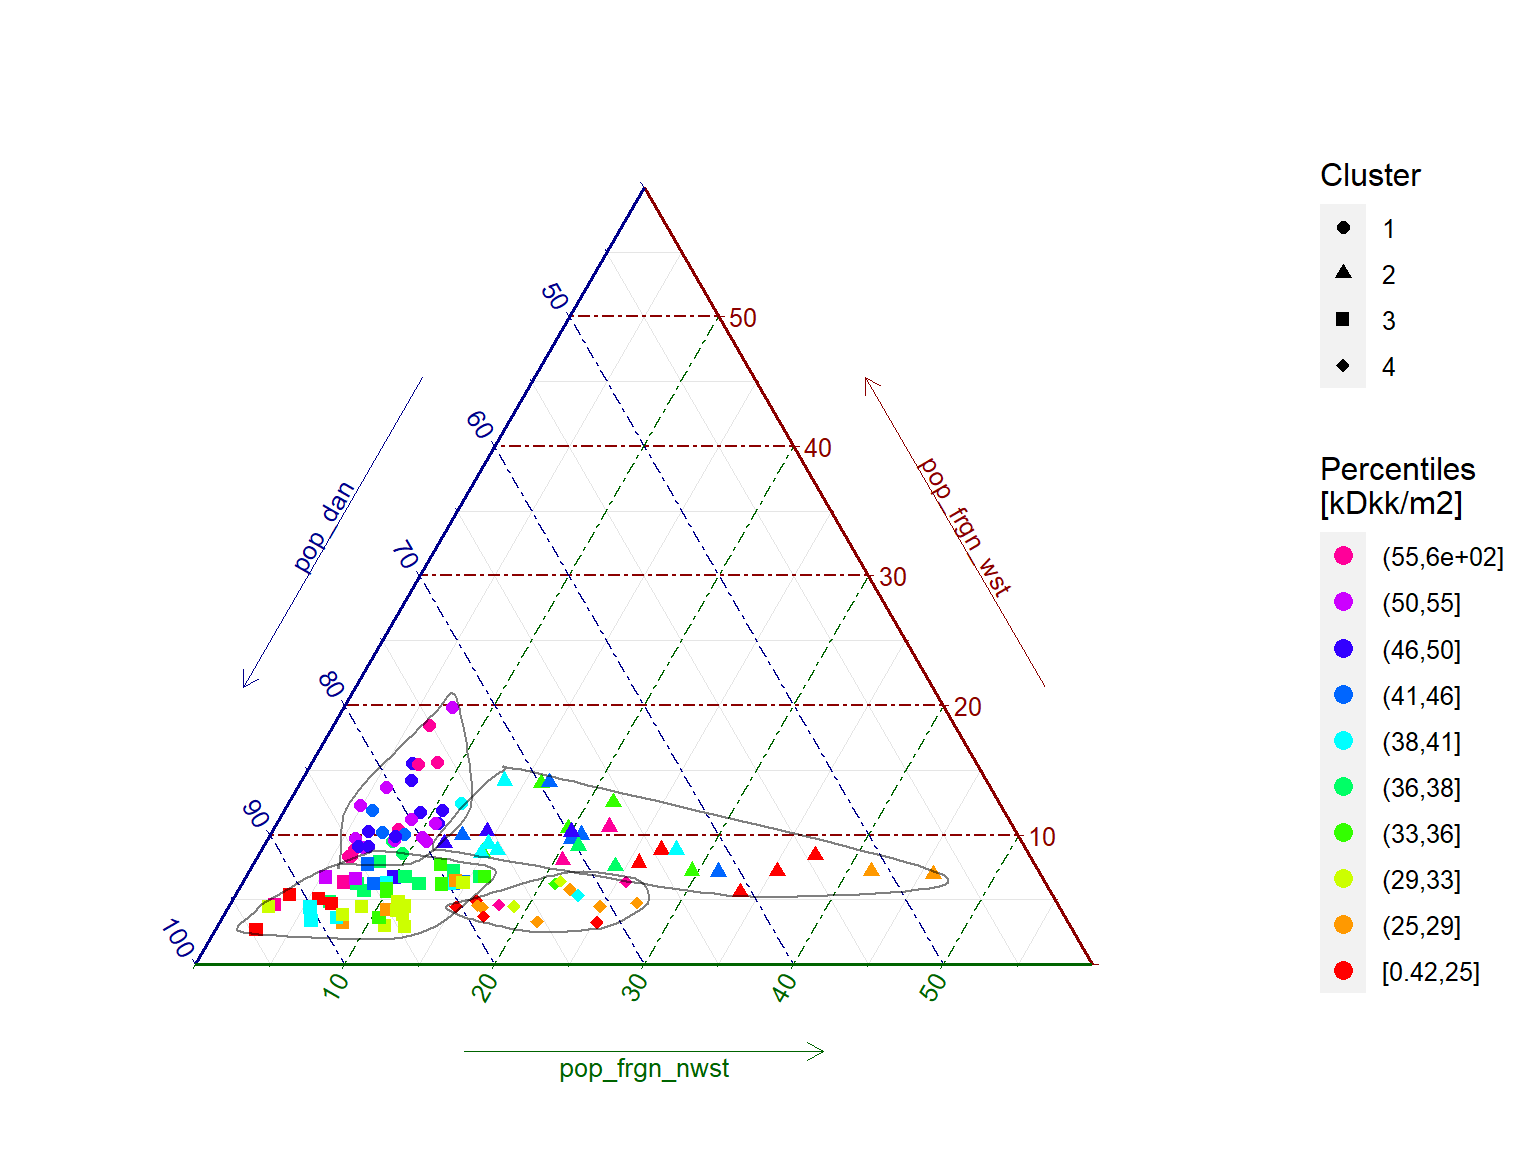
\includegraphics[width=1\linewidth]{CoDa_migr_cph_files/figure-latex/fig-tern-pop-prices-1} 

}

\caption{Ternary diagram of population distribution vs. housing prices}\label{fig:fig-tern-pop-prices}
\end{figure}

\hypertarget{linear-model}{%
\subsubsection{Linear model}\label{linear-model}}

\begin{Shaded}
\begin{Highlighting}[]
\CommentTok{\# Compositional data with prices }
\NormalTok{dat\_acomp\_prices }\OtherTok{\textless{}{-}}\NormalTok{ sum\_runits\_oft\_prices }\SpecialCharTok{\%\textgreater{}\%}
  \FunctionTok{select}\NormalTok{(prsh\_id, median\_kDKK\_m2, pop\_dan, pop\_frgn\_nwst, pop\_frgn\_wst) }\SpecialCharTok{\%\textgreater{}\%}
  \FunctionTok{rename}\NormalTok{(}\AttributeTok{dan =}\NormalTok{ pop\_dan, }
         \AttributeTok{nwst =}\NormalTok{ pop\_frgn\_nwst,}
         \AttributeTok{wst =}\NormalTok{ pop\_frgn\_wst) }\SpecialCharTok{\%\textgreater{}\%} 
  \FunctionTok{as\_tibble}\NormalTok{() }\SpecialCharTok{\%\textgreater{}\%}
  \FunctionTok{drop\_na}\NormalTok{() }\SpecialCharTok{\%\textgreater{}\%} 
  \CommentTok{\# Close dataset}
  \FunctionTok{clo}\NormalTok{(}\AttributeTok{parts =} \FunctionTok{c}\NormalTok{(}\StringTok{"dan"}\NormalTok{, }\StringTok{"nwst"}\NormalTok{, }\StringTok{"wst"}\NormalTok{),}
      \AttributeTok{total =} \DecValTok{100}\NormalTok{) }\SpecialCharTok{\%\textgreater{}\%} 
  \CommentTok{\# CoDa}
  \FunctionTok{acomp}\NormalTok{()}

\CommentTok{\# First balance ratio nwst/dan+wst}
\NormalTok{bal1   }\OtherTok{\textless{}{-}} \FunctionTok{balance}\NormalTok{(dat\_acomp\_prices , }\SpecialCharTok{\textasciitilde{}}\NormalTok{dan}\SpecialCharTok{/}\NormalTok{wst}\SpecialCharTok{/}\NormalTok{nwst) }\SpecialCharTok{\%\textgreater{}\%} \FunctionTok{as\_tibble}\NormalTok{() }\SpecialCharTok{\%\textgreater{}\%}\NormalTok{ janitor}\SpecialCharTok{::}\FunctionTok{clean\_names}\NormalTok{()}
\NormalTok{dat\_m1 }\OtherTok{\textless{}{-}}\NormalTok{ sum\_runits\_oft\_prices  }\SpecialCharTok{\%\textgreater{}\%} \FunctionTok{bind\_cols}\NormalTok{(bal1)}
\NormalTok{lm1    }\OtherTok{\textless{}{-}} \FunctionTok{lm}\NormalTok{(}\FunctionTok{log}\NormalTok{(median\_kDKK\_m2) }\SpecialCharTok{\textasciitilde{}}\NormalTok{ danwst\_nwst  }\SpecialCharTok{+}\NormalTok{ dan\_wst, }\AttributeTok{data =}\NormalTok{ dat\_m1)}

\CommentTok{\# First balance ratio wst/dan+nwst}
\NormalTok{bal2   }\OtherTok{\textless{}{-}} \FunctionTok{balance}\NormalTok{(dat\_acomp\_prices , }\SpecialCharTok{\textasciitilde{}}\NormalTok{dan}\SpecialCharTok{/}\NormalTok{nwst}\SpecialCharTok{/}\NormalTok{wst) }\SpecialCharTok{\%\textgreater{}\%} \FunctionTok{as\_tibble}\NormalTok{() }\SpecialCharTok{\%\textgreater{}\%}\NormalTok{ janitor}\SpecialCharTok{::}\FunctionTok{clean\_names}\NormalTok{()}
\NormalTok{dat\_m2 }\OtherTok{\textless{}{-}}\NormalTok{ sum\_runits\_oft\_prices  }\SpecialCharTok{\%\textgreater{}\%} \FunctionTok{bind\_cols}\NormalTok{(bal2)}
\NormalTok{lm2    }\OtherTok{\textless{}{-}} \FunctionTok{lm}\NormalTok{(}\FunctionTok{log}\NormalTok{(median\_kDKK\_m2) }\SpecialCharTok{\textasciitilde{}}\NormalTok{ dannwst\_wst  }\SpecialCharTok{+}\NormalTok{ dan\_nwst, }\AttributeTok{data =}\NormalTok{ dat\_m2)}

\CommentTok{\# First balance ratio dan/wst+nwst}
\NormalTok{bal3   }\OtherTok{\textless{}{-}} \FunctionTok{balance}\NormalTok{(dat\_acomp\_prices , }\SpecialCharTok{\textasciitilde{}}\NormalTok{nwst}\SpecialCharTok{/}\NormalTok{wst}\SpecialCharTok{/}\NormalTok{dan) }\SpecialCharTok{\%\textgreater{}\%} \FunctionTok{as\_tibble}\NormalTok{() }\SpecialCharTok{\%\textgreater{}\%}\NormalTok{ janitor}\SpecialCharTok{::}\FunctionTok{clean\_names}\NormalTok{()}
\NormalTok{dat\_m3 }\OtherTok{\textless{}{-}}\NormalTok{ sum\_runits\_oft\_prices  }\SpecialCharTok{\%\textgreater{}\%} \FunctionTok{bind\_cols}\NormalTok{(bal3)}
\NormalTok{lm3    }\OtherTok{\textless{}{-}} \FunctionTok{lm}\NormalTok{(}\FunctionTok{log}\NormalTok{(median\_kDKK\_m2) }\SpecialCharTok{\textasciitilde{}}\NormalTok{ nwstwst\_dan  }\SpecialCharTok{+}\NormalTok{ nwst\_wst, }\AttributeTok{data =}\NormalTok{ dat\_m3)}
\end{Highlighting}
\end{Shaded}

Regression coefficients:

\begin{Shaded}
\begin{Highlighting}[]
\NormalTok{slm1 }\OtherTok{\textless{}{-}} \FunctionTok{summary}\NormalTok{(lm1) }\SpecialCharTok{\%\textgreater{}\%} \FunctionTok{prettify}\NormalTok{()}
\NormalTok{slm2 }\OtherTok{\textless{}{-}} \FunctionTok{summary}\NormalTok{(lm2) }\SpecialCharTok{\%\textgreater{}\%} \FunctionTok{prettify}\NormalTok{()}
\NormalTok{slm3 }\OtherTok{\textless{}{-}} \FunctionTok{summary}\NormalTok{(lm3) }\SpecialCharTok{\%\textgreater{}\%} \FunctionTok{prettify}\NormalTok{()}

\FunctionTok{bind\_rows}\NormalTok{(slm1[}\DecValTok{2}\NormalTok{,], slm2[}\DecValTok{2}\NormalTok{,], slm3[}\DecValTok{2}\NormalTok{,]) }\SpecialCharTok{\%\textgreater{}\%} 
  \FunctionTok{rename}\NormalTok{(}\AttributeTok{model =} \StringTok{" "}\NormalTok{) }\SpecialCharTok{\%\textgreater{}\%} 
  \FunctionTok{mutate}\NormalTok{(}\AttributeTok{model =} \FunctionTok{case\_when}\NormalTok{(}
\NormalTok{    model }\SpecialCharTok{==} \StringTok{"danwst\_nwst"} \SpecialCharTok{\textasciitilde{}} \StringTok{"Model 1 (dan \& wst vs. nwst)"}\NormalTok{,}
\NormalTok{    model }\SpecialCharTok{==} \StringTok{"dannwst\_wst"} \SpecialCharTok{\textasciitilde{}} \StringTok{"Model 2 (dan \& nwst vs. wst)"}\NormalTok{,}
\NormalTok{    model }\SpecialCharTok{==} \StringTok{"nwstwst\_dan"} \SpecialCharTok{\textasciitilde{}} \StringTok{"Model 3 (nwst \& wst vs. dan)"}
\NormalTok{  )) }\SpecialCharTok{\%\textgreater{}\%} 
  \FunctionTok{kbl}\NormalTok{(}\AttributeTok{caption =} \StringTok{"Regression coefficient (β) of pivot coordinates"}\NormalTok{,}
      \AttributeTok{digits =} \DecValTok{3}\NormalTok{) }\SpecialCharTok{\%\textgreater{}\%}
  \FunctionTok{kable\_styling}\NormalTok{()}
\end{Highlighting}
\end{Shaded}

\begin{table}

\caption{\label{tab:tbl-prsh-CoDa-house-prices-lm}Regression coefficient (ß) of pivot coordinates}
\centering
\begin{tabular}[t]{l|r|r|r|r|r|l|l}
\hline
model & Estimate & CI (lower) & CI (upper) & Std. Error & t value & Pr(>|t|) &    \\
\hline
Model 1 (dan \& wst vs. nwst) & 0.359 & 0.166 & 0.551 & 0.097 & 3.683 & <0.001 & ***\\
\hline
Model 2 (dan \& nwst vs. wst) & -0.430 & -0.699 & -0.162 & 0.136 & -3.170 & 0.002 & **\\
\hline
Model 3 (nwst \& wst vs. dan) & 0.072 & -0.217 & 0.360 & 0.146 & 0.494 & 0.622 & \\
\hline
\end{tabular}
\end{table}

\begin{Shaded}
\begin{Highlighting}[]
\FunctionTok{check\_model}\NormalTok{(lm1)}
\end{Highlighting}
\end{Shaded}

\begin{center}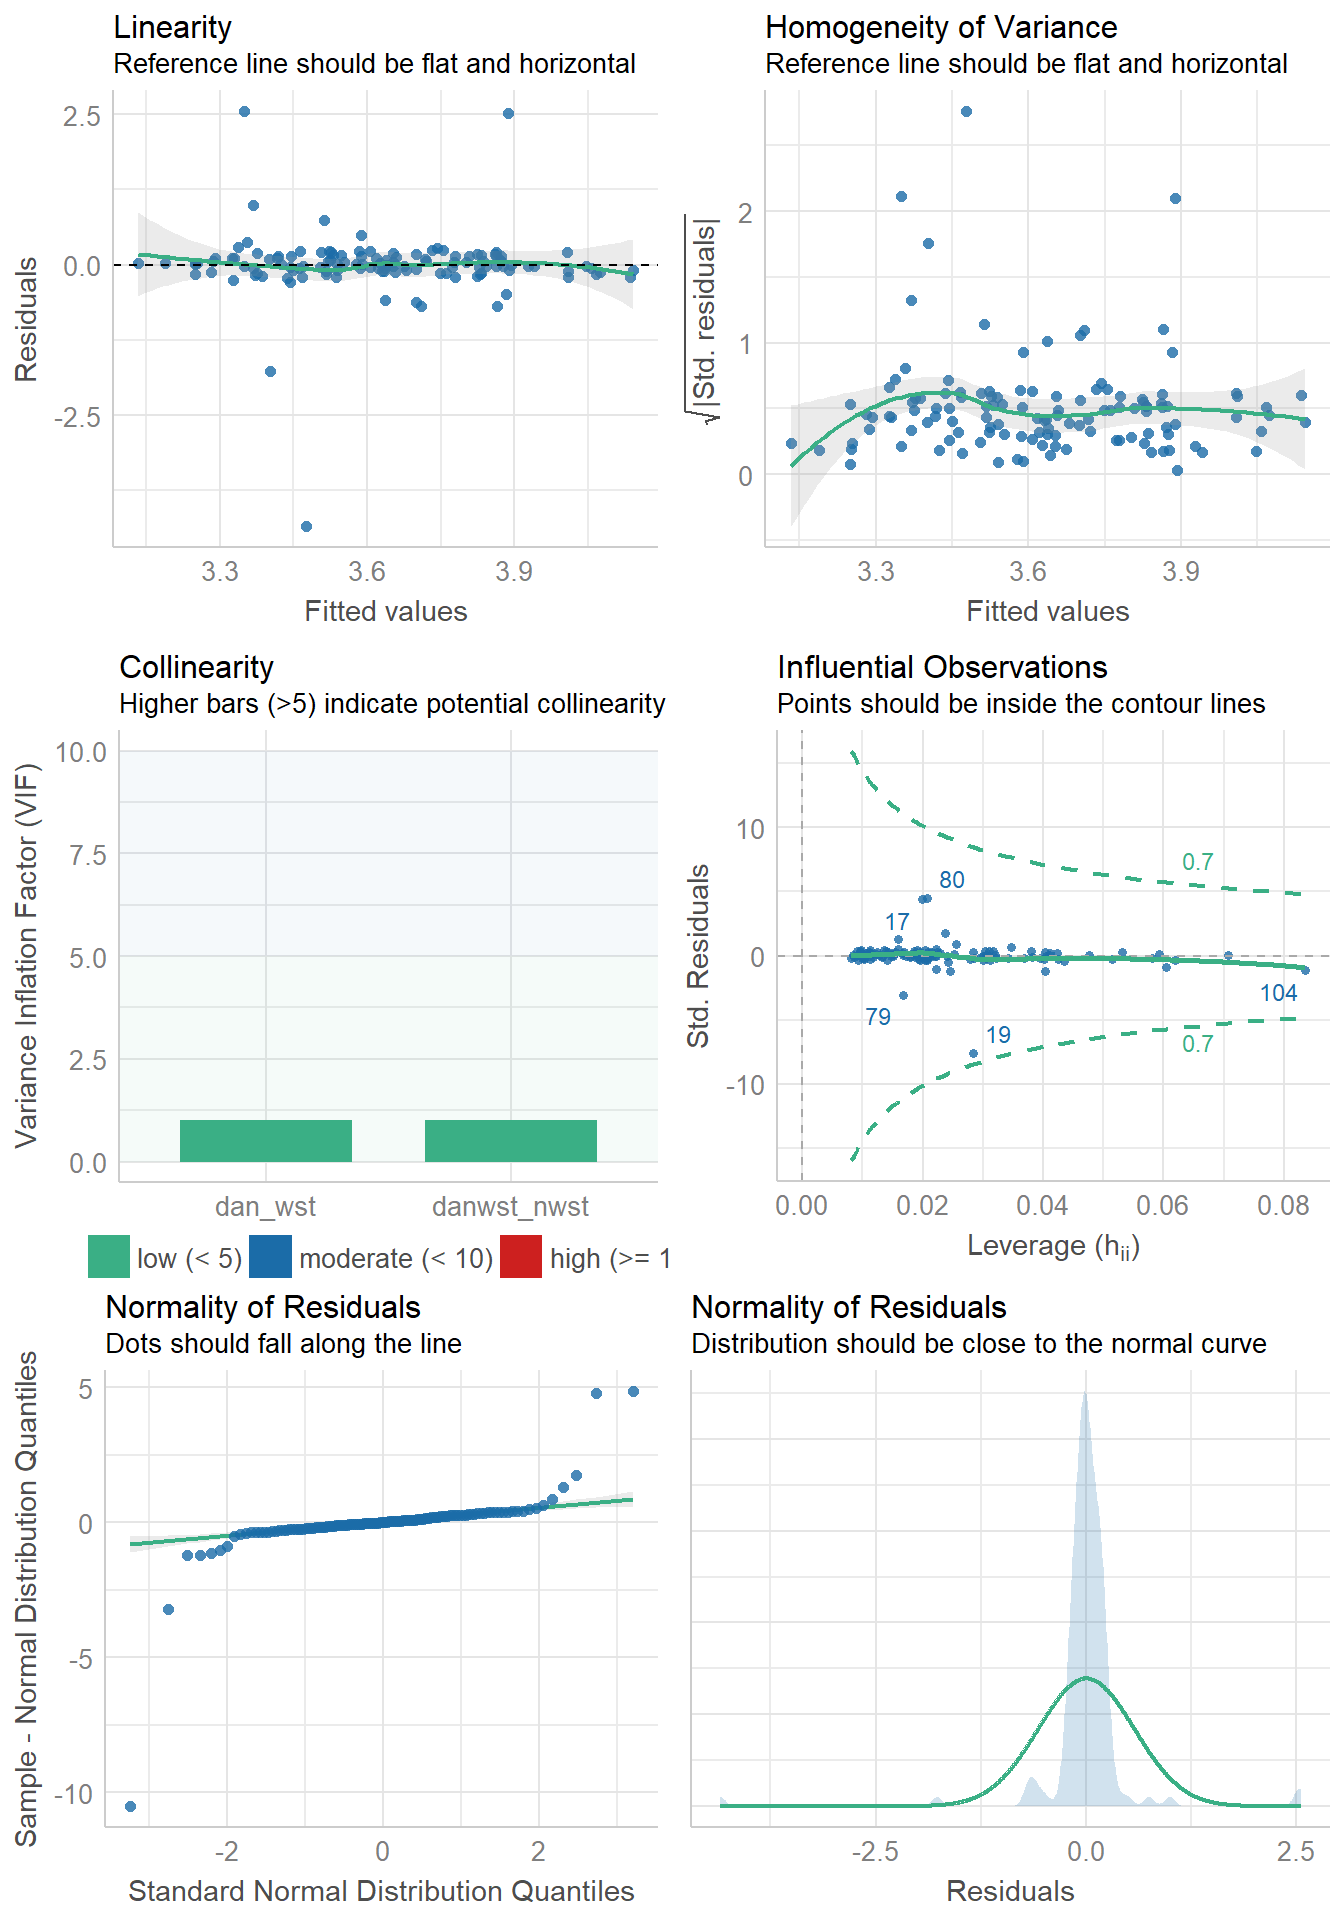
\includegraphics{CoDa_migr_cph_files/figure-latex/check-model-1} \end{center}

Values vs.~predictions:

\begin{Shaded}
\begin{Highlighting}[]
\NormalTok{sum\_runits\_oft\_prices}\SpecialCharTok{$}\NormalTok{pred1 }\OtherTok{\textless{}{-}} \FunctionTok{predict}\NormalTok{(lm1)}

\FunctionTok{ggplot}\NormalTok{() }\SpecialCharTok{+}
  \FunctionTok{geom\_point}\NormalTok{(}\AttributeTok{data =}\NormalTok{ sum\_runits\_oft\_prices,}
             \FunctionTok{aes}\NormalTok{(}\AttributeTok{x =}\NormalTok{ pred1,}
                 \AttributeTok{y =} \FunctionTok{log}\NormalTok{(median\_kDKK\_m2))) }\SpecialCharTok{+}
  \FunctionTok{scale\_x\_continuous}\NormalTok{(}\AttributeTok{name =} \StringTok{"Prediction"}\NormalTok{) }\SpecialCharTok{+}
  \FunctionTok{scale\_y\_continuous}\NormalTok{(}\AttributeTok{name =} \StringTok{"log(HP)"}\NormalTok{) }\SpecialCharTok{+}
  \FunctionTok{geom\_abline}\NormalTok{(}\AttributeTok{intercept =} \DecValTok{0}\NormalTok{,}
              \AttributeTok{slope =} \DecValTok{1}\NormalTok{,}
              \AttributeTok{colour =} \StringTok{"red"}\NormalTok{)}
\end{Highlighting}
\end{Shaded}

\begin{figure}[H]

{\centering 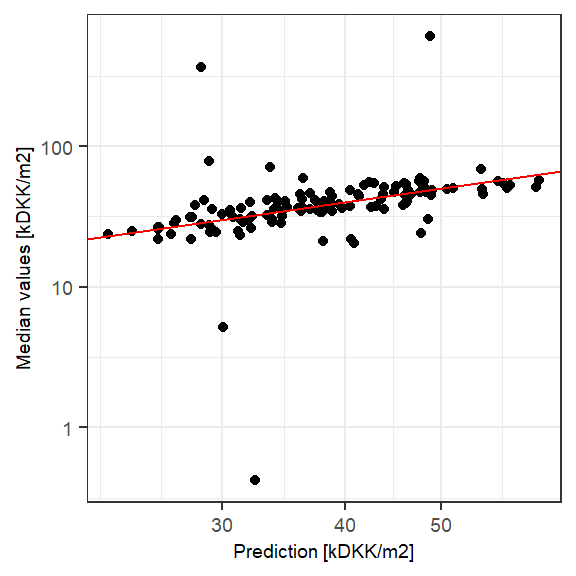
\includegraphics{CoDa_migr_cph_files/figure-latex/fig-prsh-CoDa-house-prices-lm-1} 

}

\caption{Predictions based on balances (b1 and b2) vs. median values (red line: x = y)}\label{fig:fig-prsh-CoDa-house-prices-lm}
\end{figure}

Predicted heat outcome:

\begin{Shaded}
\begin{Highlighting}[]
\DocumentationTok{\#\# Heat map (ternary diagram)}
\CommentTok{\# Compute a grid of points in the simplex space}
\NormalTok{dan }\OtherTok{\textless{}{-}}\NormalTok{ wst }\OtherTok{\textless{}{-}} \FunctionTok{seq}\NormalTok{(}\FloatTok{0.5}\NormalTok{, }\FloatTok{99.5}\NormalTok{, }\AttributeTok{length.out =} \DecValTok{100}\NormalTok{)}
\NormalTok{df }\OtherTok{\textless{}{-}} \FunctionTok{expand\_grid}\NormalTok{(}\AttributeTok{dan =}\NormalTok{ dan, }\AttributeTok{wst =}\NormalTok{ wst) }\SpecialCharTok{\%\textgreater{}\%}  
  \FunctionTok{mutate}\NormalTok{(}\AttributeTok{nwst =} \DecValTok{100} \SpecialCharTok{{-}}\NormalTok{ dan }\SpecialCharTok{{-}}\NormalTok{ wst) }\SpecialCharTok{\%\textgreater{}\%} 
  \FunctionTok{filter}\NormalTok{(nwst }\SpecialCharTok{\textgreater{}=} \DecValTok{0}\NormalTok{)}

\CommentTok{\# ilr transformation to transform into a prediction grid on real space}
\NormalTok{df\_bal }\OtherTok{\textless{}{-}}\NormalTok{ df }\SpecialCharTok{\%\textgreater{}\%} 
  \CommentTok{\# Close dataset}
  \FunctionTok{clo}\NormalTok{(}\AttributeTok{parts =} \FunctionTok{c}\NormalTok{(}\StringTok{"dan"}\NormalTok{, }\StringTok{"wst"}\NormalTok{, }\StringTok{"nwst"}\NormalTok{),}
      \AttributeTok{total =} \DecValTok{100}\NormalTok{) }\SpecialCharTok{\%\textgreater{}\%} 
  \CommentTok{\# CoDa}
  \FunctionTok{acomp}\NormalTok{() }\SpecialCharTok{\%\textgreater{}\%} 
  \CommentTok{\# Balances}
  \FunctionTok{balance}\NormalTok{(}\SpecialCharTok{\textasciitilde{}}\NormalTok{dan}\SpecialCharTok{/}\NormalTok{wst}\SpecialCharTok{/}\NormalTok{nwst) }\SpecialCharTok{\%\textgreater{}\%}
  \FunctionTok{as\_tibble}\NormalTok{() }\SpecialCharTok{\%\textgreater{}\%}
\NormalTok{  janitor}\SpecialCharTok{::}\FunctionTok{clean\_names}\NormalTok{()}

\NormalTok{df }\OtherTok{\textless{}{-}}\NormalTok{ df }\SpecialCharTok{\%\textgreater{}\%} \FunctionTok{bind\_cols}\NormalTok{(df\_bal)}

\CommentTok{\# Predict the outcome (with model 1)}
\NormalTok{df\_pred }\OtherTok{\textless{}{-}} \FunctionTok{predict}\NormalTok{(lm1, }\AttributeTok{newdata =}\NormalTok{ df, }\AttributeTok{se.fit =} \ConstantTok{TRUE}\NormalTok{)}
\NormalTok{df }\OtherTok{\textless{}{-}} \FunctionTok{bind\_cols}\NormalTok{(df, df\_pred)}

\CommentTok{\# Back{-}transform prediction to the original scale}
\NormalTok{df }\OtherTok{\textless{}{-}}\NormalTok{ df }\SpecialCharTok{\%\textgreater{}\%} 
     \FunctionTok{mutate}\NormalTok{(}\AttributeTok{fit\_LCI =}\NormalTok{ fit }\SpecialCharTok{{-}} \FloatTok{1.96} \SpecialCharTok{*} \FunctionTok{sqrt}\NormalTok{(}\FloatTok{0.5} \SpecialCharTok{*}\NormalTok{ se.fit}\SpecialCharTok{\^{}}\DecValTok{2}\NormalTok{),}
            \AttributeTok{fit\_UCI =}\NormalTok{ fit }\SpecialCharTok{+} \FloatTok{1.96} \SpecialCharTok{*} \FunctionTok{sqrt}\NormalTok{(}\FloatTok{0.5} \SpecialCharTok{*}\NormalTok{ se.fit}\SpecialCharTok{\^{}}\DecValTok{2}\NormalTok{),}
            \CommentTok{\# back{-}transform}
            \AttributeTok{HP\_pred =} \FunctionTok{exp}\NormalTok{(fit }\SpecialCharTok{+} \FloatTok{0.5}\SpecialCharTok{*}\NormalTok{se.fit}\SpecialCharTok{\^{}}\DecValTok{2}\NormalTok{),}
            \AttributeTok{HP\_LCI  =} \FunctionTok{exp}\NormalTok{(fit\_LCI }\SpecialCharTok{+} \FloatTok{0.5}\SpecialCharTok{*}\NormalTok{se.fit}\SpecialCharTok{\^{}}\DecValTok{2}\NormalTok{),}
            \AttributeTok{HP\_UCI  =} \FunctionTok{exp}\NormalTok{(fit\_UCI }\SpecialCharTok{+} \FloatTok{0.5}\SpecialCharTok{*}\NormalTok{se.fit}\SpecialCharTok{\^{}}\DecValTok{2}\NormalTok{)}
\NormalTok{     )}

\DocumentationTok{\#\# Transects for piloting predictions along with 95\% confidence intervals at}
\CommentTok{\# e.g. Start in the mean composition (D = 80\%, wst = 7.5\%; nwst = 12.5\%)}

\CommentTok{\# a) HP variation with nwst when log{-}ratio(dan/wst) = log(80/7.5) = c1 }
\NormalTok{c1 }\OtherTok{\textless{}{-}} \FunctionTok{log}\NormalTok{(}\DecValTok{80}\SpecialCharTok{/}\FloatTok{7.5}\NormalTok{)}
\NormalTok{tran1 }\OtherTok{\textless{}{-}} \FunctionTok{tibble}\NormalTok{(}\AttributeTok{name =} \StringTok{"tran1"}\NormalTok{,}
                \AttributeTok{nwst =} \FunctionTok{seq}\NormalTok{(}\DecValTok{1}\NormalTok{, }\DecValTok{99}\NormalTok{, }\DecValTok{1}\NormalTok{),}
                \AttributeTok{wst =}\NormalTok{ (}\DecValTok{100} \SpecialCharTok{{-}}\NormalTok{ nwst)}\SpecialCharTok{/}\NormalTok{(}\DecValTok{1} \SpecialCharTok{+} \FunctionTok{exp}\NormalTok{(c1)), }
                \AttributeTok{dan =} \DecValTok{100} \SpecialCharTok{{-}}\NormalTok{ nwst }\SpecialCharTok{{-}}\NormalTok{ wst)}

\CommentTok{\# b) HP variation with wst when log{-}ratio(dan/nwst) = log(80/12.5) = c2}
\NormalTok{c2 }\OtherTok{\textless{}{-}} \FunctionTok{log}\NormalTok{(}\DecValTok{80}\SpecialCharTok{/}\FloatTok{12.5}\NormalTok{)}
\NormalTok{tran2 }\OtherTok{\textless{}{-}} \FunctionTok{tibble}\NormalTok{(}\AttributeTok{name =} \StringTok{"tran2"}\NormalTok{,}
                \AttributeTok{wst =} \FunctionTok{seq}\NormalTok{(}\DecValTok{1}\NormalTok{, }\DecValTok{99}\NormalTok{, }\DecValTok{1}\NormalTok{),}
                \AttributeTok{nwst =}\NormalTok{ (}\DecValTok{100} \SpecialCharTok{{-}}\NormalTok{ wst)}\SpecialCharTok{/}\NormalTok{(}\DecValTok{1} \SpecialCharTok{+} \FunctionTok{exp}\NormalTok{(c2)), }
                \AttributeTok{dan =} \DecValTok{100} \SpecialCharTok{{-}}\NormalTok{ nwst }\SpecialCharTok{{-}}\NormalTok{ wst)}

\CommentTok{\# Combine in one tibble}
\NormalTok{tran }\OtherTok{\textless{}{-}} \FunctionTok{bind\_rows}\NormalTok{(tran1, tran2)}

\CommentTok{\# ilr transformation}
\NormalTok{tran }\OtherTok{\textless{}{-}}\NormalTok{ tran }\SpecialCharTok{\%\textgreater{}\%} 
  \FunctionTok{mutate}\NormalTok{(}\AttributeTok{danwst\_nwst =} \FunctionTok{sqrt}\NormalTok{(}\DecValTok{2}\SpecialCharTok{/}\DecValTok{3}\NormalTok{) }\SpecialCharTok{*} \FunctionTok{log}\NormalTok{( }\FunctionTok{sqrt}\NormalTok{(dan }\SpecialCharTok{*}\NormalTok{ wst) }\SpecialCharTok{/}\NormalTok{ nwst),}
         \AttributeTok{dan\_wst =} \FunctionTok{sqrt}\NormalTok{(}\DecValTok{1}\SpecialCharTok{/}\DecValTok{2}\NormalTok{) }\SpecialCharTok{*} \FunctionTok{log}\NormalTok{(dan }\SpecialCharTok{/}\NormalTok{ wst))}

\CommentTok{\# Predictions}
\NormalTok{tran\_pred }\OtherTok{\textless{}{-}} \FunctionTok{predict}\NormalTok{(lm1, tran, }\AttributeTok{se.fit =}\NormalTok{ T, }\AttributeTok{level =} \FloatTok{0.95}\NormalTok{) }\SpecialCharTok{\%\textgreater{}\%} 
  \FunctionTok{as\_tibble}\NormalTok{() }\SpecialCharTok{\%\textgreater{}\%} 
  \CommentTok{\# back{-}transform to original scale}
  \FunctionTok{mutate}\NormalTok{(}\AttributeTok{fit\_LCI =}\NormalTok{ fit }\SpecialCharTok{{-}} \FloatTok{1.96} \SpecialCharTok{*} \FunctionTok{sqrt}\NormalTok{(}\FloatTok{0.5} \SpecialCharTok{*}\NormalTok{ se.fit}\SpecialCharTok{\^{}}\DecValTok{2}\NormalTok{),}
         \AttributeTok{fit\_UCI =}\NormalTok{ fit }\SpecialCharTok{+} \FloatTok{1.96} \SpecialCharTok{*} \FunctionTok{sqrt}\NormalTok{(}\FloatTok{0.5} \SpecialCharTok{*}\NormalTok{ se.fit}\SpecialCharTok{\^{}}\DecValTok{2}\NormalTok{),}
         \CommentTok{\# back{-}transform}
         \AttributeTok{HP\_pred =} \FunctionTok{exp}\NormalTok{(fit }\SpecialCharTok{+} \FloatTok{0.5}\SpecialCharTok{*}\NormalTok{se.fit}\SpecialCharTok{\^{}}\DecValTok{2}\NormalTok{),}
         \AttributeTok{HP\_LCI  =} \FunctionTok{exp}\NormalTok{(fit\_LCI }\SpecialCharTok{+} \FloatTok{0.5}\SpecialCharTok{*}\NormalTok{se.fit}\SpecialCharTok{\^{}}\DecValTok{2}\NormalTok{),}
         \AttributeTok{HP\_UCI  =} \FunctionTok{exp}\NormalTok{(fit\_UCI }\SpecialCharTok{+} \FloatTok{0.5}\SpecialCharTok{*}\NormalTok{se.fit}\SpecialCharTok{\^{}}\DecValTok{2}\NormalTok{))}

\CommentTok{\# Add predictions to the table}
\NormalTok{tran }\OtherTok{\textless{}{-}} \FunctionTok{bind\_cols}\NormalTok{(tran, tran\_pred) }
\end{Highlighting}
\end{Shaded}

\begin{Shaded}
\begin{Highlighting}[]
\CommentTok{\# Ternary plot showing the predicted outcome for different compositions}
\NormalTok{p }\OtherTok{\textless{}{-}} \FunctionTok{ggtern}\NormalTok{(df,}\FunctionTok{aes}\NormalTok{(dan, wst, nwst)) }\SpecialCharTok{+} 
  \FunctionTok{geom\_hex\_tern}\NormalTok{(}\AttributeTok{binwidth  =} \FloatTok{0.005}\NormalTok{, }
                \FunctionTok{aes}\NormalTok{(}\AttributeTok{value =}\NormalTok{ HP\_pred),}
                \AttributeTok{fun =}\NormalTok{ mean,}
                \AttributeTok{alpha =} \FloatTok{0.75}\NormalTok{) }\SpecialCharTok{+}
  \FunctionTok{scale\_fill\_gradientn}\NormalTok{(}\AttributeTok{name =} \StringTok{"Predicted HP}\SpecialCharTok{\textbackslash{}n}\StringTok{[kDkk/m2]"}\NormalTok{,}
                       \AttributeTok{colours =} \FunctionTok{rainbow}\NormalTok{(}\DecValTok{10}\NormalTok{), }
                       \AttributeTok{trans =} \StringTok{"log10"}\NormalTok{) }\SpecialCharTok{+}
\NormalTok{  ggtern}\SpecialCharTok{::}\FunctionTok{theme\_rgbw}\NormalTok{() }\SpecialCharTok{+}
\NormalTok{  ggtern}\SpecialCharTok{::}\FunctionTok{theme\_hidetitles}\NormalTok{() }\SpecialCharTok{+}
  \CommentTok{\# ggtern::theme\_zoom\_L(0.6) +}
\NormalTok{  ggalt}\SpecialCharTok{::}\FunctionTok{geom\_encircle}\NormalTok{(}\AttributeTok{data =}\NormalTok{ sum\_runits\_oft\_prices,}
                       \FunctionTok{aes}\NormalTok{(}\AttributeTok{x =}\NormalTok{ pop\_dan,}
                           \AttributeTok{y =}\NormalTok{ pop\_frgn\_wst,}
                           \AttributeTok{z =}\NormalTok{ pop\_frgn\_nwst,}
                           \AttributeTok{shape =}\NormalTok{ CL4),}
                       \AttributeTok{size =} \DecValTok{1}\NormalTok{,}
                       \AttributeTok{alpha =} \FloatTok{0.5}\NormalTok{,}
                       \AttributeTok{expand =} \FloatTok{0.01}\NormalTok{,}
                       \AttributeTok{inherit.aes =} \ConstantTok{FALSE}\NormalTok{) }

\CommentTok{\# Add transects}
\NormalTok{p }\SpecialCharTok{+} \FunctionTok{geom\_line}\NormalTok{(}\AttributeTok{data =}\NormalTok{ tran,}
              \FunctionTok{aes}\NormalTok{(}\AttributeTok{x =}\NormalTok{ dan,}
                  \AttributeTok{y =}\NormalTok{ wst,}
                  \AttributeTok{z =}\NormalTok{ nwst,}
                  \AttributeTok{colour =}\NormalTok{ name,}
                  \AttributeTok{linetype =}\NormalTok{ name),}
              \AttributeTok{size =} \DecValTok{1}\NormalTok{) }\SpecialCharTok{+}
  \FunctionTok{scale\_linetype\_manual}\NormalTok{(}\AttributeTok{name =} \StringTok{"Transects"}\NormalTok{,}
                        \AttributeTok{values =} \FunctionTok{c}\NormalTok{(}\StringTok{"dashed"}\NormalTok{, }\StringTok{"solid"}\NormalTok{)) }\SpecialCharTok{+}
  \FunctionTok{scale\_colour\_manual}\NormalTok{(}\AttributeTok{name =} \StringTok{"Transects"}\NormalTok{,}
                      \AttributeTok{values =} \FunctionTok{c}\NormalTok{(}\StringTok{"\#0072B2"}\NormalTok{, }\StringTok{"\#D55E00"}\NormalTok{)) }
\end{Highlighting}
\end{Shaded}

\begin{figure}[H]

{\centering 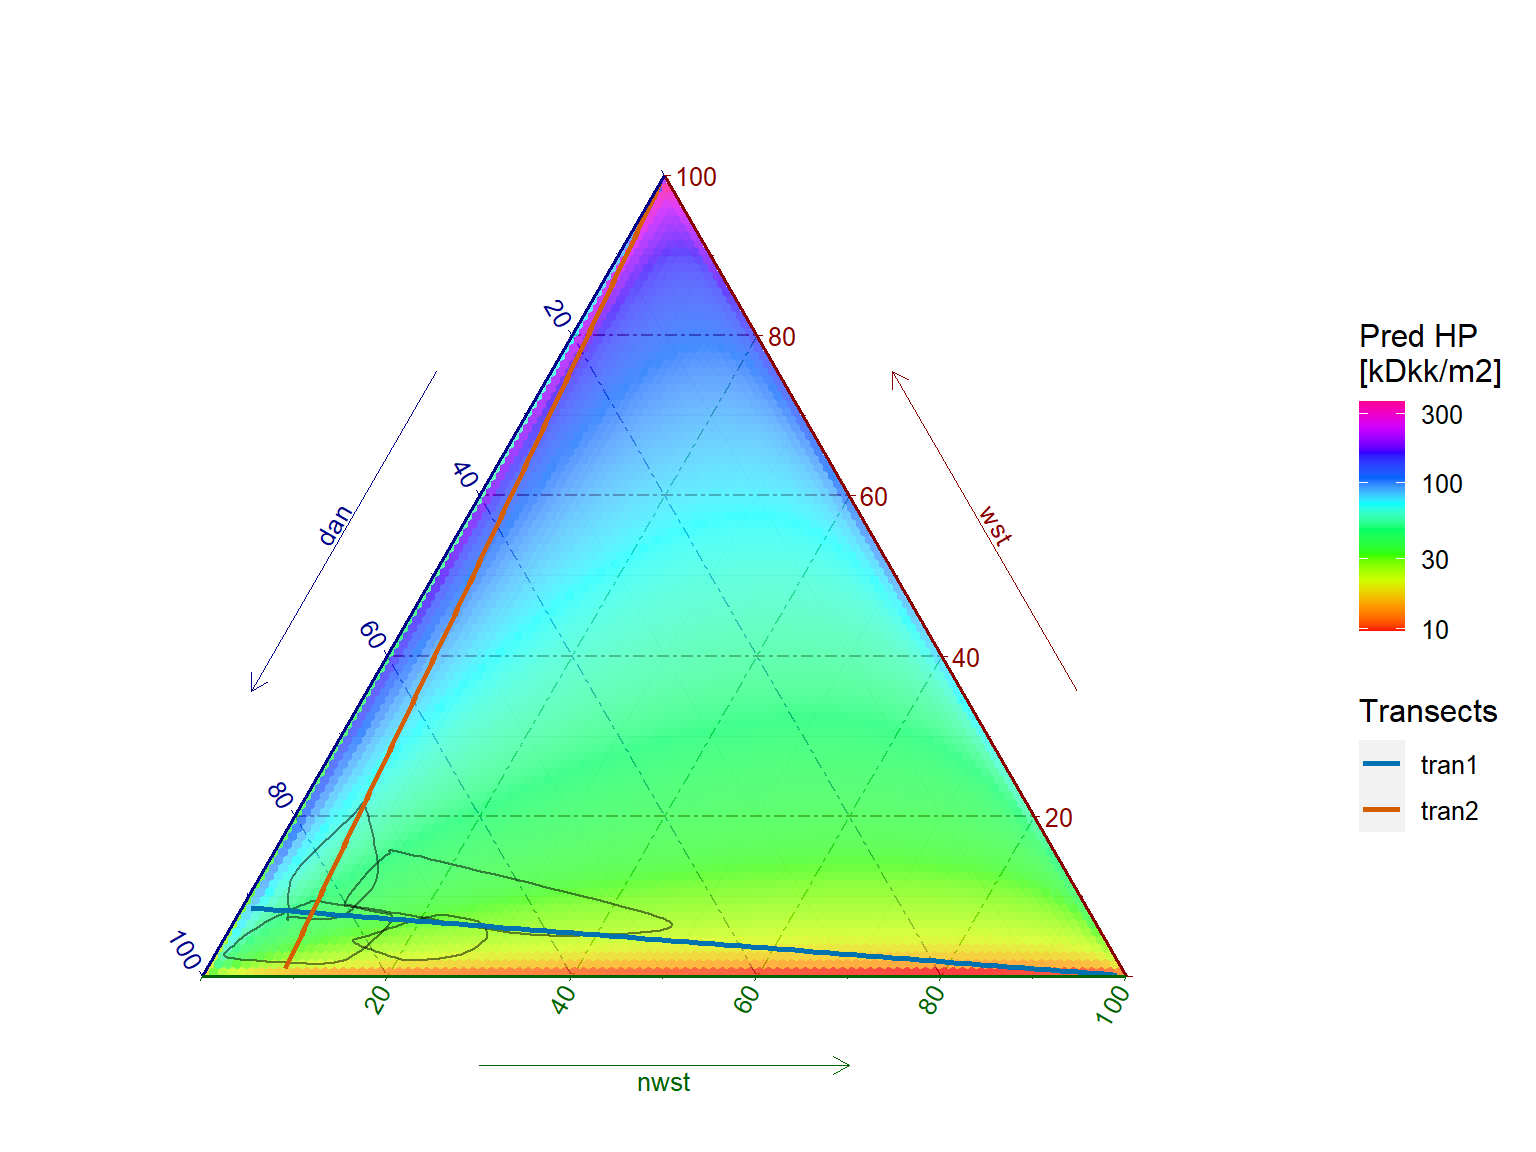
\includegraphics[width=1\linewidth]{CoDa_migr_cph_files/figure-latex/fig-pred-CoDa-lm-1} 

}

\caption{Ternary plot showing the predicted outcome for different compositions}\label{fig:fig-pred-CoDa-lm}
\end{figure}

Predictions with CI:

\begin{Shaded}
\begin{Highlighting}[]
\NormalTok{p1 }\OtherTok{\textless{}{-}}\NormalTok{ tran }\SpecialCharTok{\%\textgreater{}\%} 
  \FunctionTok{filter}\NormalTok{(name }\SpecialCharTok{==} \StringTok{"tran1"}\NormalTok{) }\SpecialCharTok{\%\textgreater{}\%} 
  \FunctionTok{ggplot}\NormalTok{(}\FunctionTok{aes}\NormalTok{(}\AttributeTok{x =}\NormalTok{ nwst, }\AttributeTok{y =}\NormalTok{ HP\_pred)) }\SpecialCharTok{+} 
  \FunctionTok{geom\_ribbon}\NormalTok{(}\FunctionTok{aes}\NormalTok{(}\AttributeTok{ymin =}\NormalTok{ HP\_LCI,}
                  \AttributeTok{ymax =}\NormalTok{ HP\_UCI),}
              \AttributeTok{alpha =} \FloatTok{0.5}\NormalTok{,}
              \AttributeTok{fill =} \StringTok{"red"}\NormalTok{) }\SpecialCharTok{+}
  \FunctionTok{geom\_line}\NormalTok{() }\SpecialCharTok{+}
  \FunctionTok{scale\_y\_log10}\NormalTok{(}\AttributeTok{limits =} \FunctionTok{c}\NormalTok{(}\DecValTok{1}\NormalTok{, }\DecValTok{2000}\NormalTok{)) }\SpecialCharTok{+}
  \FunctionTok{labs}\NormalTok{(}\AttributeTok{title =} \StringTok{"Transect 1: log(Danes/Western) = 2.367"}\NormalTok{,}
       \AttributeTok{x =} \StringTok{"nwst [\%]"}\NormalTok{,}
       \AttributeTok{y =} \StringTok{"HP [kDKK/m2]"}\NormalTok{) }\SpecialCharTok{+}
  \FunctionTok{annotation\_logticks}\NormalTok{(}\AttributeTok{sides =} \StringTok{"l"}\NormalTok{)}

\NormalTok{p2 }\OtherTok{\textless{}{-}}\NormalTok{ tran }\SpecialCharTok{\%\textgreater{}\%} 
  \FunctionTok{filter}\NormalTok{(name }\SpecialCharTok{==} \StringTok{"tran2"}\NormalTok{) }\SpecialCharTok{\%\textgreater{}\%} 
  \FunctionTok{ggplot}\NormalTok{(}\FunctionTok{aes}\NormalTok{(}\AttributeTok{x =}\NormalTok{ wst, }\AttributeTok{y =}\NormalTok{ HP\_pred)) }\SpecialCharTok{+} 
  \FunctionTok{geom\_ribbon}\NormalTok{(}\FunctionTok{aes}\NormalTok{(}\AttributeTok{ymin =}\NormalTok{ HP\_LCI,}
                  \AttributeTok{ymax =}\NormalTok{ HP\_UCI),}
              \AttributeTok{alpha =} \FloatTok{0.5}\NormalTok{,}
              \AttributeTok{fill =} \StringTok{"red"}\NormalTok{) }\SpecialCharTok{+}
  \FunctionTok{geom\_line}\NormalTok{() }\SpecialCharTok{+}
  \FunctionTok{scale\_y\_log10}\NormalTok{(}\AttributeTok{limits =} \FunctionTok{c}\NormalTok{(}\DecValTok{1}\NormalTok{, }\DecValTok{2000}\NormalTok{)) }\SpecialCharTok{+}
  \FunctionTok{labs}\NormalTok{(}\AttributeTok{title =} \StringTok{"Transect 2: log(Danes/non{-}Western) = 1.856"}\NormalTok{,}
       \AttributeTok{x =} \StringTok{"wst [\%]"}\NormalTok{,}
       \AttributeTok{y =} \StringTok{"HP [kDKK/m2]"}\NormalTok{) }\SpecialCharTok{+} 
  \FunctionTok{annotation\_logticks}\NormalTok{(}\AttributeTok{sides =} \StringTok{"l"}\NormalTok{)}

\NormalTok{p1 }\SpecialCharTok{+}\NormalTok{ p2}
\end{Highlighting}
\end{Shaded}

\textbackslash begin\{figure\}{[}H{]}

\{\centering 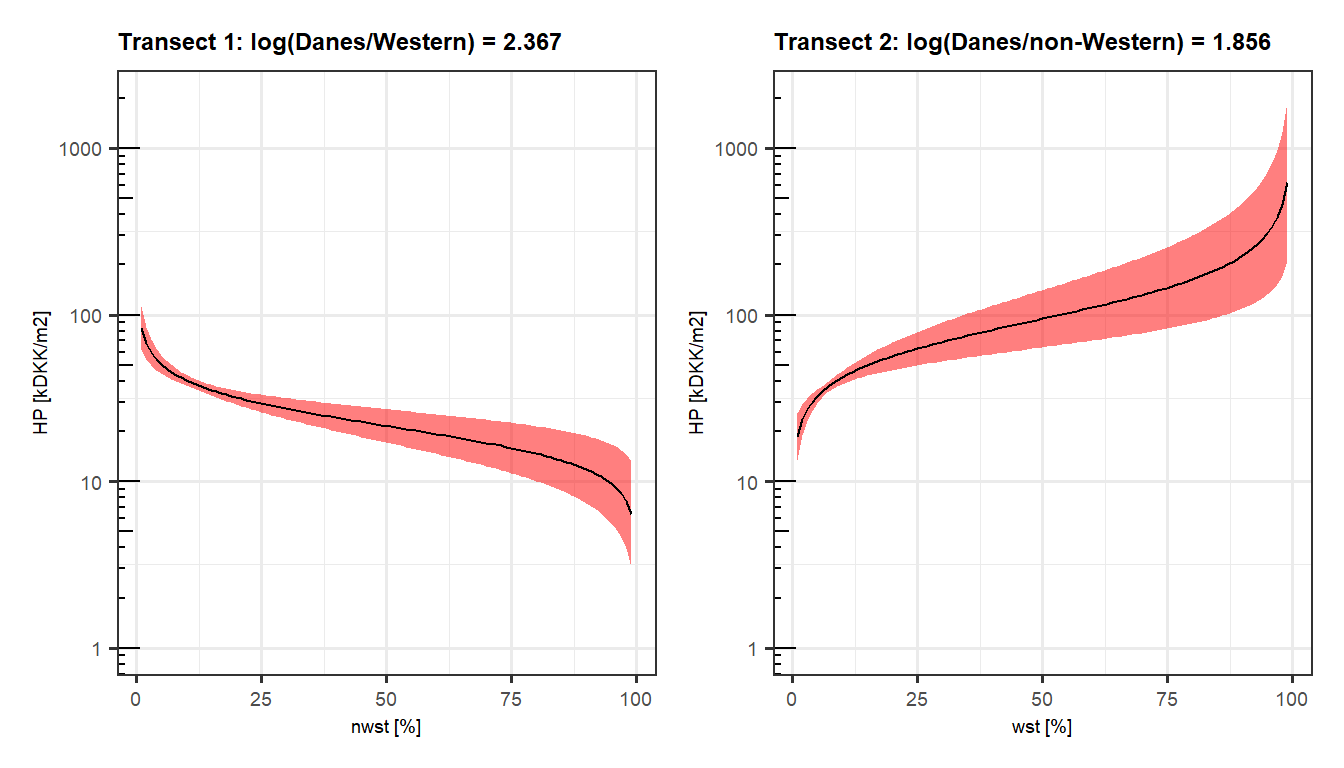
\includegraphics[width=1\linewidth]{CoDa_migr_cph_files/figure-latex/fig-transects-pred-CI-1}

\}

\textbackslash caption\{Predicted median house prices at parish level
with 95\% CI for transects 1 and 2\}\label{fig:fig-transects-pred-CI}
\textbackslash end\{figure\}

\hypertarget{acknowledgements}{%
\section{Acknowledgements}\label{acknowledgements}}

This work has been financed by Aalborg University - AAU (Project:
\href{https://www.flow.aau.dk/}{Global flows of migrants and their
impact on north European welfare states - FLOW}). The sole
responsibility of this publication lies with the authors. AAU is not
responsible for any use that may be made of the information contained
therein.

\hypertarget{r-session}{%
\section{R session}\label{r-session}}

\begin{verbatim}
## R version 4.1.2 (2021-11-01)
## Platform: x86_64-w64-mingw32/x64 (64-bit)
## Running under: Windows 10 x64 (build 19042)
## 
## Matrix products: default
## 
## locale:
## [1] LC_COLLATE=English_United Kingdom.1252 
## [2] LC_CTYPE=English_United Kingdom.1252   
## [3] LC_MONETARY=English_United Kingdom.1252
## [4] LC_NUMERIC=C                           
## [5] LC_TIME=English_United Kingdom.1252    
## 
## attached base packages:
## [1] stats     graphics  grDevices datasets  utils     methods   base     
## 
## other attached packages:
##  [1] dangeo_0.0.0.9000  devtools_2.4.2     usethis_2.0.1      ggsflabel_0.0.1   
##  [5] tm_0.7-8           NLP_0.2-1          tidytable_0.6.3    forcats_0.5.1     
##  [9] stringr_1.4.0      dplyr_1.0.7        purrr_0.3.4        readr_1.4.0       
## [13] tidyr_1.1.3        tibble_3.1.2       tidyverse_1.3.1    viridis_0.6.1     
## [17] viridisLite_0.4.0  units_0.7-2        tricolore_1.2.2    spdep_1.1-8       
## [21] spData_0.3.10      sp_1.4-5           sf_1.0-1           remotes_2.4.0     
## [25] rmarkdown_2.9      performance_0.7.3  papeR_1.0-5        xtable_1.8-4      
## [29] car_3.0-11         carData_3.0-4      patchwork_1.1.1    modelr_0.1.8      
## [33] knitr_1.33         kableExtra_1.3.4   ggtern_3.3.5       ggplot2_3.3.5     
## [37] gtsummary_1.4.2    ggspatial_1.1.5    furrr_0.2.3        future_1.21.0     
## [41] dint_2.1.3         danstat_0.1.0      data.table_1.14.0  broom_0.7.8       
## [45] compositions_2.0-2
## 
## loaded via a namespace (and not attached):
##   [1] utf8_1.2.1          proto_1.0.0         tidyselect_1.1.1   
##   [4] grid_4.1.2          munsell_0.5.0       effectsize_0.4.5   
##   [7] codetools_0.2-18    withr_2.4.2         colorspace_2.0-2   
##  [10] ggalt_0.4.0         rstudioapi_0.13     robustbase_0.93-8  
##  [13] bayesm_3.1-4        Rttf2pt1_1.3.9      listenv_0.8.0      
##  [16] labeling_0.4.2      slam_0.1-48         datawizard_0.1.0   
##  [19] farver_2.1.0        rprojroot_2.0.2     coda_0.19-4        
##  [22] parallelly_1.27.0   LearnBayes_2.15.1   vctrs_0.3.8        
##  [25] generics_0.1.0      xfun_0.24           R6_2.5.1           
##  [28] cachem_1.0.5        assertthat_0.2.1    scales_1.1.1       
##  [31] gtable_0.3.0        ash_1.0-15          globals_0.14.0     
##  [34] processx_3.5.2      qqplotr_0.0.5       rlang_0.4.11       
##  [37] systemfonts_1.0.2   splines_4.1.2       extrafontdb_1.0    
##  [40] hexbin_1.28.2       yaml_2.2.1          abind_1.4-5        
##  [43] backports_1.2.1     extrafont_0.17      tensorA_0.36.2     
##  [46] tools_4.1.2         ellipsis_0.3.2      raster_3.4-13      
##  [49] RColorBrewer_1.1-2  proxy_0.4-26        ggridges_0.5.3     
##  [52] sessioninfo_1.1.1   latex2exp_0.5.0     Rcpp_1.0.7         
##  [55] plyr_1.8.6          classInt_0.4-3      ps_1.6.0           
##  [58] prettyunits_1.1.1   deldir_0.2-10       haven_2.4.1        
##  [61] ggrepel_0.9.1       fs_1.5.0            magrittr_2.0.1     
##  [64] openxlsx_4.2.4      gmodels_2.18.1      reprex_2.0.0       
##  [67] pkgload_1.2.1       hms_1.1.0           evaluate_0.14      
##  [70] rio_0.5.27          readxl_1.3.1        gridExtra_2.3      
##  [73] testthat_3.0.4      compiler_4.1.2      maps_3.3.0         
##  [76] KernSmooth_2.23-20  gt_0.3.0            crayon_1.4.1       
##  [79] htmltools_0.5.1.1   mgcv_1.8-38         expm_0.999-6       
##  [82] lubridate_1.7.10    DBI_1.1.1           dbplyr_2.1.1       
##  [85] proj4_1.0-10.1      see_0.6.4           MASS_7.3-54        
##  [88] broom.helpers_1.3.0 rappdirs_0.3.3      boot_1.3-28        
##  [91] Matrix_1.3-4        cli_3.0.1           gdata_2.18.0       
##  [94] parallel_4.1.2      insight_0.14.2      pkgconfig_2.0.3    
##  [97] foreign_0.8-81      xml2_1.3.2          svglite_2.0.0      
## [100] webshot_0.5.2       rvest_1.0.0         snakecase_0.11.0   
## [103] callr_3.7.0         digest_0.6.27       parameters_0.14.0  
## [106] janitor_2.1.0       cellranger_1.1.0    curl_4.3.2         
## [109] gtools_3.9.2        lifecycle_1.0.0     nlme_3.1-153       
## [112] jsonlite_1.7.2      desc_1.3.0          fansi_0.5.0        
## [115] labelled_2.8.0      pillar_1.6.2        lattice_0.20-45    
## [118] fastmap_1.1.0       httr_1.4.2          DEoptimR_1.0-9     
## [121] pkgbuild_1.2.0      survival_3.2-13     glue_1.4.2         
## [124] bayestestR_0.10.5   zip_2.2.0           class_7.3-19       
## [127] stringi_1.6.2       memoise_2.0.0       renv_0.14.0        
## [130] e1071_1.7-7
\end{verbatim}

\end{document}
